\documentclass[12pt]{uthesis-v12}  %---> DO NOT ALTER THIS COMMAND
\usepackage{amsmath}
\usepackage{mathtools}
\usepackage{epigraph}
\usepackage{cancel}
\usepackage{xcolor}
\newcommand\Ccancel[2][black]{\renewcommand\CancelColor{\color{#1}}\cancel{#2}}
\usepackage{algorithm}
\usepackage{graphicx}
\usepackage[noend]{algpseudocode}
\usepackage{gnuplot-lua-tikz}
\begin{document} %---> %---> %---> %---> DO NOT ALTER THIS COMMAND

%--------+----------------------------------------------------------+
%        |  \title{}                                    (REQUIRED)  |
%        |  \author{}                                   (REQUIRED)  |
%        |                                                          |
%        |  See section 3.1 of "Read_Me_First_(v12).pdf"            |
%        |                                                          |
%        |  Also see section 2.2 of above "Read Me" file for the    |
%        |  proper use of the invisible tilde ("~") character when  |
%        |  entering a middle initial in the \author command.       |
%        +----------------------------------------------------------+

\title{ Verification and Validation Method for 
\protect\\an Acoustic Mode Prediction Code for Turbomachinery Noise}

\author{Jeffrey Severino} 
%--------+----------------------------------------------------------+
%        |  \copyrightpage{}                            (REQUIRED)  |
%        |                                                          |
%        |  See section 3.2 of "Read_Me_First_(v12).pdf"            |
%        |                                                          |
%        |  1) You must enter either "yes" or "no" in this          |
%        |      command.  Inputting "yes" produces a copyright      |
%        |      notification page as the second page and inputting  |
%        |      "no" produces a blank second page.                  |
%        |  2) Input to this command is case sensitive.             |
%        |  3) Default: the "yes" option.                           |
%        +----------------------------------------------------------+

\copyrightpage{yes}

%--------+----------------------------------------------------------+
%        |  \mydocument{}                               (REQUIRED)  |
%        |                                                          |
%        |  See section 3.3 of "Read_Me_First_(v12).pdf"            |
%        |                                                          |
%        |  1) Input to this command is limited to the following    |
%        |     three options: a) Dissertation                       |
%        |                    b) Thesis                             |
%        |                    c) Project                            |
%        |  2) Input to this command is case-sensitive.             |
%        +----------------------------------------------------------+

\mydocument{Thesis}

%--------+----------------------------------------------------------+
%        |  \degree{}{}                                 (REQUIRED)  |
%        |                                                          |
%        |  See section 3.4 of "Read_Me_First_(v12).pdf"            |
%        |                                                          |
%        |  You need to provide two distinct inputs into this       |
%        |  command:                                                |
%        |     1) In the first set of braces you need to specify    |
%        |        the *exact* degree you will receive. Some         |
%        |        examples are: -) Masters of Arts                  |
%        |                      -) Masters of Science               |
%        |                      -) Doctor of Philosophy             |
%        |     2) In the second set of braces you need to state the |
%        |        *specific* discipline or area for that degree     |
%        |        (e.g., Economics, Education, Engineering, etc.).  |
%        |  Students should consult their advisor if they have any  |
%        |  questions about this information.                       |
%        +----------------------------------------------------------+

\degree{Masters of Science}{Mechanical Engineering}

%--------+----------------------------------------------------------+
%        |  \conferraldate{}{}                          (REQUIRED)  |
%        |                                                          |
%        |  See section 3.5 of "Read_Me_First_(v12).pdf"            |
%        |                                                          |
%        |  In the two set of braces enter the month and then the   |
%        |  year your degree will be *conferred* by the university. |
%        +----------------------------------------------------------+

\conferraldate{May}{2022}

%--------+----------------------------------------------------------+
%        |  \advisor{}                                  (REQUIRED)  |
%        |                                                          |
%        |  See section 3.6.2 of "Read_Me_First_(v12).pdf"          |
%        |                                                          |
%        |  1) Also see section 2.2 of "Read_Me_First_(v12).pdf"    |
%        |     for the proper use of the invisible tilde ("~")      |
%        |     character when entering a middle initial or the      |
%        |     abbreviation of an academic title (e.g., Dr.) in     |
%        |     the \advisor{} command.                              |
%        |  2) Also see section 3.6.1. for consistent presentation  |
%        |     of title page signature lines.                       |
%        +----------------------------------------------------------+

\advisor{Dr.~Ray Hixon}

%--------+----------------------------------------------------------+
%        |  Committee Member Signature Commands         (OPTIONAL)  |
%        |                                                          |
%        |  See section 3.6.3 of "Read_Me_First_(v12).pdf"          |
%        |                                                          |
%        |  1) Use the commands below to provide signature lines    |
%        |     for your "other" committee members;                  |
%        |        --> you must list your other committee members    |
%        |            in alphabetic order by last name              |
%        |        --> to do this, use the commands below in the     |
%        |            order presented below.                        |
%        |  2) You can choose to include none, some, or all of the  |
%        |     "XXXmember" commands below --- based on the number   |
%        |     committee members you have; simply delete (or        |
%        |     comment-out) any of the commands below that are not  |
%        |     needed.                                              |
%        |  3) Do not include the name of your committee chair or   |
%        |     the Graduate Dean in the commands listed below.      |
%        |     Their signature lines are generated by the           |
%        |     \advisor{} and \graduatedean{}{} commands.           |
%        |  4) You cannot use any of the commands below more than   |
%        |     once. (For details on this issue, see section 3.6.3  |
%        |     of "Read_Me_First_(v12).pdf".)                       |
%        |  5) Also see section 2.2 of "Read_Me_First_(v12).pdf"    |
%        |     for the proper use of the invisible tilde ("~")      |
%        |     character when entering a middle initial or the      |
%        |     abbreviation of an academic title (e.g., Dr.) in     |
%        |     the commands below.                                  |
%        |  6) See section 3.6.1. for consistent presentation of    |
%        |     title page signature lines.                          |
%        |                                                          |
%        |  I know I shouldn't have to say this, but enough         |
%        |  students over the years have made the same mistake      |
%        |  that I'm forced to state:                               |
%        |                                                          |
%        |      THE NAMES USED IN THE FOLLOWING COMMANDS ARE        |
%        |      SILLY NAMES I'VE USED AS EXAMPLES ONLY.  THEY       |
%        |      ARE NOT THE ACTUAL NAMES OF YOUR COMMITTEE          |
%        |      MEMBERS.  REPLACE THE SILLY NAMES BELOW WITH        |
%        |      THE NAMES OF YOUR ACTUAL COMMITTEE MEMBERS.         |
%        |                                                          |
%        +----------------------------------------------------------+

  \secondmember{Dr.~Chinhua Sheng}
%   \thirdmember{Dr.~Chris P.~Bacon}
%  \fourthmember{Dr.~Adam Baum}
%   \fifthmember{Dr.~Corey O.~Graff}
%   \sixthmember{Dr.~Hugh Jass}
% \seventhmember{Dr.~Noah Lott}
%  \eighthmember{Dr.~Jean Poole}
%
%--------+----------------------------------------------------------+
%        |  \graduatedean{}{}                           (REQUIRED)  |
%        |                                                          |
%        |  See section 3.6.4 of "Read_Me_First_(v12).pdf"          |
%        |                                                          |
%        |  1) THE NAME AND TITLE PROVIDED BELOW ARE THOSE OF THE   |
%        |     ACTUAL GRADUATE DEAN AT THE TIME THIS DOCUMENT WAS   |
%        |     CONSTRUCTED (January 2012). Contact the Graduate     |
%        |     College to determine whether this information is     |
%        |     correct at the time you submit your document.        |
%        |  2) Section 2.2 of "Read_Me_First_(v12).pdf" describes   |
%        |     the proper use of the invisible tilde ("~")          |
%        |     character when entering a middle initial or the      |
%        |     abbreviation of an academic title (e.g., Dr.) in     |
%        |     the \graduatedean{} command.                         |
%        |  3) See section 3.6.1. for consistent presentation of    |
%        |     title page signature lines.                          |
%        +----------------------------------------------------------+

\graduatedean{Dr.~Patricia R.~Komuniecki}{Dean}

%--------+----------------------------------------------------------+
%        |  \maketitle                                  (REQUIRED)  |
%        |                                                          |
%        |  See section 3.7 of "Read_Me_First_(v12).pdf"            |
%        |                                                          |
%        |  This is a required LaTeX command; to be brief, bad      |
%        |  things will happen if this command is not included      |
%        |  in your document at this particular location.           |
%        +----------------------------------------------------------+

\maketitle  %---->  ----->  ---->  ---->   DO NOT ALTER THIS COMMAND

%--------+----------------------------------------------------------+
%        |  Abstract Page Environment                   (REQUIRED)  |
%        |                                                          |
%        |  See section 3.8 of "Read_Me_First_(v12).pdf"            |
%        +----------------------------------------------------------+

\begin{abstractpage}
Over the last 20 years, there has been an increase in computational fluid dynamic 
codes that have made numerical analysis more and more readily available, allowing
turbomachine designers to create more novel designs. However, as airport noise
limitations become more restrictive over time, reducing aircraft 
takeoff and landing noise remains a prominent issue in the aviation community. 
One popular method to reduce aircraft noise is using acoustic liners placed on 
the walls of the engine inlet and exhaust ducts. These liners are designed to 
reduce the amplitude of acoustic modes emanating from the bypass fan as they 
propagate through the engine. The SWIRL code is a frequency-domain linearized 
Euler equation solver that is designed to predict the effect of acoustic liners
on acoustic modes propagating in realistic sheared and swirling mean flows, guiding
the design of more efficient liner configurations. The purpose of this study is
to validate SWIRL using the Method Of Manufactured Solutions (MMS). This study 
also investigated the effect of the integration and spatial differencing methods 
on the convergence for a given Manufactured Solution. In addition, the effect 
of boundary condition implementation was tested.  The improved MMS convergence
rates shown for these tests suggest that the revised SWIRL code provides more 
accurate solutions with less computational effort than the original formulation.



\end{abstractpage}

%--------+----------------------------------------------------------+
%        |  Dedication Page Environment                 (OPTIONAL)  |
%        |                                                          |
%        |  See section 3.9 of "Read_Me_First_(v12).pdf"            |
%        |                                                          |
%        |  If both a dedication page and an acknowledgements page  |
%        |  are included in the document, the dedication page must  |
%        |  proceed the acknowledgements page.                      |
%        +----------------------------------------------------------+

\begin{dedication}
\noindent For my friends and family, who have always believed in my potential 
when I did not believe it myself. 
\end{dedication}

%--------+----------------------------------------------------------+
%        |  Acknowledgments Page Environment            (OPTIONAL)  |
%        |                                                          |
%        |  See section 3.10 of "Read_Me_First_(v12).pdf"           |
%        |                                                          |
%        |  If both a dedication page and an acknowledgements page  |
%        |  are included in the document, the dedication page must  |
%        |  proceed the acknowledgements page.                      |
%        +----------------------------------------------------------+

\begin{acknowledgments}
\noindent This work is supported by the NASa Advanced Air Transport Technologies
(AATT) Project. I would like to thank Edmane Envia(?) of the NASA Glenn Research Center, who
is the technical monitor of this work. 
A very special thanks goes to Dr. Ray Hixon who supervised and guided me through
out my course work and Master's Thesis. His rigor and tenacity in his profession has 
been the model example for an aspiring aeroacoustician. 
I would like to also thank all of my committee members, Dr. Chunhua Sheng and 
Dr. Sorin Cioc. Their contributions have been instrumental. Thanks to Dr. Clifford
Brown for his programatic insights. 

I would also like to thank my focus group peers, Zaid Sabri, and Matthew Gibbons 
for their patience and support over the years. I wish them the best in all of 
their endevours.
I would also like to thank Copper Moon Coffee Shop for the endless supply of caffine 
and conversations.


\end{acknowledgments}

%--------+----------------------------------------------------------+
%        |  \tableofcontents                            (REQUIRED)  |
%        |  \listoftables                            (CONDITIONAL)  |
%        |  \listoffigures                           (CONDITIONAL)  |
%        |                                                          |
%        |  See sections 3.11 & 3.12 of "Read_Me_First_(v12).pdf"   |
%        |                                                          |
%        |  1) You must include the \tableofcontents command in     |
%        |     your document: the UT Manual requires every          |
%        |     dissertation/thesis to have a detailed table of      |
%        |     contents.                                            |
%        |  2) Including the \listoftables and \listoffigures       |
%        |     commands is "conditional."  See sections 3.12 of     |
%        |     "Read_Me_First_(v12).pdf" for additional details.    |
%        +----------------------------------------------------------+

\tableofcontents  %----->  ----->  ---->  DO NOT ALTER THIS COMMAND
\listoftables \listoffigures
\begin{listofsymbols}
    \emblem{$A$        }{mean flow speed of sound}
    \emblem{$A_T      $}{speed of sound at the duct radius}
    \emblem{$\tilde{A}$}{dimensionless speed of sound, $\frac{A}{A_T}$}
    \emblem{$D/Dt$     }{material derivative, $\partial/\partial t + V \cdot \nabla $}
    \emblem{$D_N$      }{derivative matrix using $N$ points}
    \emblem{$\textbf{e}_x$,$\textbf{e}_{\theta}$ }{s}
\end{listofsymbols}
%--------+----------------------------------------------------------+
%        |  \captionformat{}                            (REQUIRED)  |
%        |                                                          |
%        |  See section 3.12.2 of "Read_Me_First_(v12).pdf"         |
%        |                                                          |
%        |  1) You are required to choose between the "hang" or     |
%        |     "align" option for this command.                     |
%        |  2) Input to this command is case sensitive.             |
%        |  3) Default: ``hang'' option.                            |
%        +----------------------------------------------------------+

\captionformat{hang}

%--------+----------------------------------------------------------+
%        |  List of Abbreviations Environment           (OPTIONAL)  |
%        |                                                          |
%        |  See section 3.13 of "Read_Me_First_(v12).pdf"           |
%        |                                                          |
%        |  1) This is an optional section; consult your advisor    |
%        |     to determine whether you need/want to include this   |
%        |     section in your document.                            |
%        |  2) If you do not want a List of Abbreviations simply    |
%        |     delete the material below (and these instructions).  |
%        |  3) If you do want a List of Abbreviations simply        |
%        |     replace the silly material below with the            |
%        |     information relevant to your document.               |
%        |     a. Within the "listofabbreviations" environment      |
%        |        below you must use a separate \abbreviation{}{}   |
%        |        command for each entry in your List of            |
%        |        Abbreviations.                                    |
%        |     b. As the examples below demonstrate, the            |
%        |        information within the first set of braces is     |
%        |        the abbreviation and the information in the       |
%        |        second set of braces is the definition of that    |
%        |        abbreviation.                                     |
%        +----------------------------------------------------------+

\begin{listofabbreviations}

 \abbreviation{ABBREV}{This is where you provide a brief
                       definition of the abbreviation ``ABBREV''}
     \abbreviation{BB}{B.B.~King}
    \abbreviation{BSE}{Bovine Spongiform Encephalopathy (Mad Cow
                       Disease)}
     \abbreviation{CB}{L.D. Caskey and J.D. Beazley, \emph{Attic
                       Vase Paintings in the Museum of Fine
                       Arts}, Boston (Oxford 1931--1963)}
    \abbreviation{GLE}{Gauss' law for electricity: $\nabla\cdot E
                       = \displaystyle\frac{\rho}{\varepsilon_0}
                       = 4\pi k \rho$}
    \abbreviation{HHS}{Department of Health and Human Services}
    \abbreviation{IaR}{I am root}

\end{listofabbreviations}

%--------+----------------------------------------------------------+
%        |  List of Symbols Environment                 (OPTIONAL)  |
%        |                                                          |
%        |  See section 3.14 of "Read_Me_First_(v12).pdf"           |
%        |                                                          |
%        |  1) This is an optional section; consult your advisor    |
%        |     to determine whether you need/want to include this   |
%        |     section in your document.                            |
%        |  2) If you do not want a List of Symbols simply delete   |
%        |     the material below (and these instructions).         |
%        |  3) If you do want a List of Symbols simply replace the  |
%        |     silly material below with the information relevant   |
%        |     to your document.                                    |
%        |       a. Within the "listofsymbols" environment below    |
%        |          you must use a separate \emblem{}{} command     |
%        |          for each entry in your List of Symbols.         |
%        |       b. As the examples below show, insert your symbol  |
%        |          within the first set of braces in the           |
%        |          \emblem{}{} command, and its definition within  |
%        |          the second set of braces.                       |
%        |       c. Use the \emblemskip command to insert a blank   |
%        |          line between different categories of symbols:   |
%        |          -) such additional spacing is required between  |
%        |             different categories of symbols;             |
%        |          -) see "Read_Me_First_(v12).pdf" for details.   |
%        +----------------------------------------------------------+

%--------+----------------------------------------------------------+
%        |  Preface Environment                         (OPTIONAL)  |
%        |                                                          |
%        |  See section 3.15 of "Read_Me_First_(v12).pdf"           |
%        +----------------------------------------------------------+

\begin{preface}
\end{preface}

%XXXXXXXXXXXXXXXXXXXXXXXXXXXXXXXXXXXXXXXXXXXXXXXXXXXXXXXXXXXXXXXXXXXX
%XXXXXXXXXXXXXXXXXXXXXXXXXXXXXXXXXXXXXXXXXXXXXXXXXXXXXXXXXXXXXXXXXXXX
%XXXXXXXXXXXXXXXXXXXXXXXXXXXXXXXXXXXXXXXXXXXXXXXXXXXXXXXXXXXXXXXXXXXX
%XXXXXXXXXXXXXXXXXXXXXXXXXXXXXXXXXXXXXXXXXXXXXXXXXXXXXXXXXXXXXXXXXXXX

%--------+----------------------------------------------------------+
%        |  \makebody                                   (REQUIRED)  |
%        |                                                          |
%        |  See section 3.16 of "Read_Me_First_(v12).pdf"           |
%        |                                                          |
%        |  This is a *required* UThesis command; again, bad        |
%        |  things will happen if this command is not included in   |
%        |  your document at this particular location --- see the   |
%        |  file "Read_Me_First_(v12).pdf" for details.             |
%        +----------------------------------------------------------+

\makebody   %------->  ------->  ------->  DO NOT ALTER THIS COMMAND

%XXXXXXXXXXXXXXXXXXXXXXXXXXXXXXXXXXXXXXXXXXXXXXXXXXXXXXXXXXXXXXXXXXXX
%XXXXXXXXXXXXXXXXXXXXXXXXXXXXXXXXXXXXXXXXXXXXXXXXXXXXXXXXXXXXXXXXXXXX
%XXXXXXXXXXXXXXXXXXXXXXXXXXXXXXXXXXXXXXXXXXXXXXXXXXXXXXXXXXXXXXXXXXXX
%XXXXXXXXXXXXXXXXXXXXXXXXXXXXXXXXXXXXXXXXXXXXXXXXXXXXXXXXXXXXXXXXXXXX

%--------+----------------------------------------------------------+
%        |  \chapter{}                                  (REQUIRED)  |
%        |                                                          |
%        |  See section 3.17 of "Read_Me_First_(v12).pdf"           |
%        |                                                          |
%        |  For guidance on using the commands \chapter{},          |
%        |  \section{}, \subsection{}, \subsubsection{}, etc., see  |
%        |  Leslie Lamport's "LaTeX: A Document Preparation         |
%        |  System." Addison Wesley: Reading Massachusetts, 1985.   |
%        +----------------------------------------------------------+
\chapter{Background}
\section{Introduction}
\section{Overview}
\subsection{Introduction of overall field and basic explaination of this topic (What)}
% I) Opening Section
%   1) Introduce the overall field 
Aircraft noise is one of the most environmentally detrimental consequences of
commercial flight. Studies suggest that exposure to aircraft noise leads
to dimished academic performance in youth, and could increase the risk of 
cardiovascular disease for populations close to airports \cite{Basner2017}. 
Although the COVID-19 pandemic reduced air panssenger trafic by 96\% between 2019 
and 2020, \cite{pandemicReport} the global aviation commmunity has proven 
to be resilliant during times of economic shock. The International Air Transport
Association (IATA) has studied the resilience of the global air passenger markets after four notable shocks to the aviation economy; 
The impact of four notable events, (1979 oil shock, 2000-2001 dot-com bust, 9/11, and the 2008 financial crisis) 
was studied by a statistical analysis of the estimated 'passenger gap' from 1950-2014. 
Data shows that approximately 72\% of the impact of the initial shock persists 
one year after the event and diminishes to just under one-fifth of the initial impact. 
Given these trends in air transportation, the need for  aviation noise  
regulation persists and will continue to be a concern so long as the aviation
continues this rate of growth.

% II) Background and overview
%      What is the current situation with aircraft noise
%      wht are acoustic modes and liners
%      Swirling flow codes
%      code verification
%   1) What is sound propagation and why is it relevant in ducted flows? 
%   2) What are the key theories and research
%   3) what is the current context and what does this mean
Since the dawn of commerical airlines in the early 20th centurty, the increased demand for aircraft transport
introduced jet engines to support large cargo and passengers. Consequently,
this rise in innovation resulted in high volume engine noise due to 
the frequency of flights. After 1975, 
efforts to reduce aircraft noise eliminated the noise pollution for 90\% of
the population \cite{FAAPolicy}.  However, given the rapid increase in
aircraft movements and consequently increase in noise exposure to larger 
populations, the advancement in noise reduction 
technologies has only been moderately increasing, leaving a requirement for 
in aeroacoustic modeling techniques and treatment strategies to compete with 
the demand for quiet subsonic flight \cite{icao2020}.  
%   2) Introduce the research problem
% The 
Between the 1950s and 1960's aero gas turbine designs shifted to higher by pass 
ratios with two or three shafts. The high by pass ratio (HBP) fan utilized multiple
stages of fans and  air streams \cite{smith1989aircraft}. The efficiency of these
engines rose with the availablility of materials that are able to cool flows
passing over the turbofan, thus slowing the overall jet velocity but maintaining the 
efficiency of the engine. One of the most popular configurations is the geared 
turbofan (GTF), the largest contributor to the noise on modern aircraft 
has been the fan upon take-off and landing.  Although the use of the GTF has
reduced the noise emissions by 75\% \cite{GTFinfo}, further noise reduction
technologies to mitigate the noise associated to the turbofans geometric
configuration and operation speeds. One of the most common techiques to reduce 
fan noise  is to include the use of acoustic treatment along the walls of the
turbomachine's nacelle. 

Due to the increase in high-bypass-ratio of turbomachines, the newest models of 
engines have a significantly larger diameter and a shorter nacelle, leaving less
room to place acoustic treatments in regions where it will be effective \cite{Kozaczuk2017}.
Figure \ref{fig:intro} shows the evolution of directivity for turbomachines as 
the use of HBR fans became more popular. As these engines continue 
to develop, an increased understanding of sound propagation within
the interstage of the engine is gong to be needed due to flow behavior (high compressibility
and rotational effects).  While a turbomachine's general flow condition includes 
a series of axial, tangential, and radial velocity components that vary
depending on the location of concern, the swirling flow between fan stages has 
been an area of interest due to the potential for acoustic treatment in a 
location previously avoided for its flow complexity. This work will explore how 
sound propagation is modeled and how the current state of code verification and 
validation currently stands. This introduction will describe how fluid mechanics
is utlized to establish an aeroacoustic model for various ducted flows. It will 
also discuss how code verification is used in the computational and numerical fields
but will show the need for the use of these code verification techniques for 
a frequency domain CAA code. 


%   3) State your research aims

%   4) Outline the introduction 

%3)
\begin{figure}
    \centering
    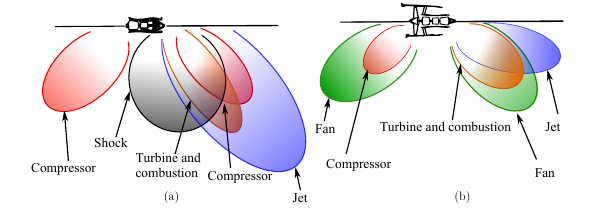
\includegraphics[width=\textwidth]{Chapter-1-Introduction/Figures/lowVhighBPRdirectivitySMITH2004.png}
    \caption{ The evolution of the directivity and the 
    relative levels of sources as a function of engine architecture (a)low bypass-ratio (b) high bypass ratio \cite{smith1989aircraft}}
    \label{fig:intro}
\end{figure}

\section{Statement of the of the research questions}
\subsection{What is already known?}
% III) Research Problem

%   1) What's already known?
%   2) What's missing?
%   3) Why is it a problem?
In general, jet engine designers can model flow within a turbomachine with 
the Navier Stokes (N-S) Equations, a set of partial differential equations that
describe the mass, momentum and energy of a given viscous fluid, however 
these equations can be computationally expensive as they are used in the most
general cases. For aeroacousticians, the N-S equations can be too complicated
to identify sound generation and propagation because acoustic waves are low 
amplitude (~ only a fraction of atmospheric pressure) and are not strongly
influenced by viscosity.   As a result, it is common in practice to 
utilize the Linearized Euler equations (LEE),
a closely related set of PDEs that model inviscid fluid, as they provide an 
approximation for higher Reynold number flows where viscosity 
does not play a critical role. A popular approach to modeling sound propagation 
within a flow is to ``linearize'' the Euler equations, which decomposes the 
flow solution into a mean and fluctuating component . The decomposition is done 
in a linear fashion because the sound propagation amplitude is small with respect
to the mean flow, and their presence does not appreciable change the mean flow 
field. The LEE provides a system of linear equations where for uniform flow, 
the solution is a family of wavenumbers and radial mode shapes that arise from 
unsteady disturbances for flows within a cylindrical duct.  Another method 
decomposes the flow into vortical and potential parts \cite{golubev1996sound}.
In either case, this presents an initial value problem which 
in limited cases can obtain analytical solutions for simplified mean flow. Once a mean flow 
is contains a tangential component, the LEE equations must be solved numerically.  
\subsection{What is missing?/Why is it a problem?}
For uniform flows in a hard wall duct , the waves are categorized as vortical 
,entropical, and acoustic waves. The vortical and entropic waves soley convect with 
the mean flow, where as the acoustic wave can propagate without damping or decay 
exponentially.  However, for swiriling flows, the waves are partially coupled
and are not easily categorized due to an additonal category of ``nearly convecting'' 
modes \cite{Kerrebrock2012},\cite{KERREBROCK1974} . 
Therefore, the families of waves must be found numerically \cite{Envia2004}
making the ducted acoustic propagtion in swirling flow a problem without
an analytical solution but has a framework for a numerical solution.
\subsection{The goal and significance of the investigation}
Swirling flow has been a difficult problem to investigate in comparison to 
flows parallel to the wall domain of a duct \cite{COOPER2001} because of the 
lack of an analytical solution and thus cannot be described from a single convective 
wave equation. However, the solution for sheared mean flows was first presented
by Goldstein \cite{Goldstein1978},\cite{Goldstein1979}. Various special cases of
swirling flow (free vortex and solid body swirl) was examined in \cite{KAPUR1973}
\cite{Kerrebrock2012}, \cite{KERREBROCK1974}. In recent years verification and
validation has been done given the rise in technologies capabale of experimentally
measuring the acoustic modes within a turbomachine \cite{Maldonado2016}. This
work aims offer additional insight to the verification and validation process 
by expanding on techniques used in this field.  
\section{Definition of the terms (if needed)}
\section{Organization of research (Structure)}
% IV) Research aims, objectives, and research question
% V) State benefit/significance
% - speed improvement 
% VI)
% VII)


This research aims to investigave the theoretical framework that is used to
model ducted sound propagation within various flow fields and apply the 
``gold-standard'' of code verification , the method of manufactured solutions 
(MMS) and method of exact solutions (MES) for the limited subset 
of equations where a solution is known, such as uniform mean flow. 


The literature review in the next chapter will discuss the governing equations that are
used to predict the acoustic behavior in a fluid flowing internally, followed 
by the research problem that arises in swirling flow, the objectives and 
questions, the significance and finally the limitations.  The proposed research aims to determine the impact of the numerical schemes used
in the swirling flow problem and how it effects the family of waves that are
produced from the problem formulation so a better understanding of the 
acoustic phenomena as the flow under goes a compressible rotational flow. The use
of the method of manufactured solutions is used as a means of ensuring the code is
correctly approximating the goverining equations and will check the effect of the numerical schemes
on the axial wavenumbers produced.
 
\section{Research Questions and Hypothesis}


- the problem that we're addressing

-- being able to conduct component level code verification tests for the problem
of characterizing the duct acoustics for flow using a LEE model.

why is it a problem? there is multiple ways of arriving at the same solution. 
This can be used to give a metric to either method for the various computational
methods that may be needed to arrive at the final answer.

In the mid 90's,an aeroacoustics model for swirling flow had been proposed and 
has bypassed using a single PDE and has instead used an eigenvalue approach on the 
four governing flow equations. (Why Is this better? does this capturE the problem
differently? why not use the PDE alone instead\ldots)

The proposed component verification from Kleb and Wood will be presented to addreess the characterization of 
modes and the presence of numerical ones. Using higher accuracy methods should 
further improve The result. another thing is to determine how many grid points are needed
for each method



\chapter{Chapter 2: Literature Review}
\chapter{Chapter 3: Theory}
\section{Divergence operations in new coordinate systems}

%\epigraph{The introduction of numbers as \textit{coordinates} is an act of violence."} {\textit{Hermann Weyl}}

%Hermann Weyl was a renown mathematician and physicist who has made revolutionary contributions to the field of differential geometry and topology. In his work on manifolds, he proposed the idea of working without coordinates and showed the application of multi-variable without the need to define a coordinate system , using coordinates when only absolutely necessary. This perspective emphasizes the distinction between quantities and the various coordinates systems that can be used to describe their change and behavior.
The divergence, ($\nabla$), represents the operation of taking derivatives of a vector field. However, understanding the mathematical and physical representation of the divergence operator into new coordinate systems serves as a good prerequisite for the application of the Navier Stokes equations for the evaluation of aerodynamic models in unusual flow domains. Although there are many resources that will provide equations in varying coordinate systems, the derivation offers insight into the advantages and drawbacks of using a new reference frame for a flow domain. The divergence operator in Cartesian coordinates is,
%This is also important because eigenmode analysis tells us the domain of a pulse traveling through the domain at a frequency that is intrinsic to the flow itself



\begin{align*}
\vec{\nabla} \equiv
\hat{e}_x \frac{\partial }{\partial x}  %...
+ \hat{e}_y \frac{\partial }{\partial y}  %...
	+ \hat{e}_z \frac{\partial }{\partial z}                      = 0
\label{Divergence_Operator}
\end{align*}

The vectors, $\hat{e}_x,\hat{e}_y,\hat{e}_z$ (commonly denoted in literature as $\hat{i}$,$\hat{j}$,$\hat{k}$) are the basis vectors of the Cartesian coordinate system. The vector hat ( $\vec{}$ ) reminds us that divergence operation includes a scalar product of  the basis vectors and the individual derivative terms themselves.
These basis vectors \textit{scale} with the derivatives $d/dx$ $d/dy$ $d/dz$ in the direction of these basis vectors themselves. This implicitly captures the coordinate system and assumptions that corresponds to the basis vectors themselves.

To relate the basis vectors of the cylindrical coordinate system to the Cartesian coordinate system, we use the following relations,
\begin{align*}
	r 
	&= \sqrt{x^2 + y^2} \\
	\theta 
	&= \tan^{-1} \Big( \frac{y}{x} \Big) \\
	&= \cos^{-1} \Big( \frac{x}{r} \Big) \\
	&=\sin^{-1} \Big( \frac{y}{r} \Big)		
\end{align*}
	Note that the equation above also establishes $x   = r\cos \theta$ and $y = r\sin\theta$. The Cartesian basis vectors are related to the cylindrical basis vectors of the new coordinate system by,

\begin{align*}
	\hat{e}_r 
	&= \hat{e}_x \cos \theta + \hat{e}_y \sin \theta \\
	\hat{e}_{\theta} 
	&= -\hat{e}_x \sin \theta + \hat{e}_y \cos \theta \\
	\hat{e}_z 	 
	&= \hat{e}_z %\label{eq:cylindrical_basis_vectors}
\end{align*}

Defining these relationships, (they'll be useful later)

\begin{align*}
	\frac{\partial \hat{e}_{r	  }}{\partial r} 
	&= \frac{\partial \hat{e}_{\theta}}{\partial r} 
	= \frac{\partial \hat{e}_{z}	   }{\partial r} = 0 \\
	\frac{\partial \hat{e}_{r	  }}{\partial \theta} 
	&=	-\hat{e}_x \sin \theta + \hat{e}_y \cos \theta                = \hat{e}_{\theta}\\
	\frac{\partial \hat{e}_{\theta	  }}{\partial \theta}
	&= -\left(
	\hat{e}_x \cos \theta + \hat{e}_y \sin \theta
	\right) = 
	-\hat{e}_{r}
\end{align*}

The multi-variable chain rule for differentiation is then used to express the Cartesian variables, $\frac{\partial}{\partial x}$,$\frac{\partial}{\partial y}$,$\frac{\partial}{\partial z}$ , with respect to the cylindrical variable.

\begin{align*}
	\frac{\partial }{\partial x}
	&= \frac{\partial }{\partial r}\frac{d r}{d x} +
	\frac{\partial }{\partial \theta}\frac{d \theta}{d x} +
	\frac{\partial }{\partial z}\frac{d z}{d x} 
	%\label{ddx}
\end{align*}

\begin{align*}
	\frac{\partial }{\partial y}
	&=
	\frac{\partial }{\partial r} 	 \frac{d r}{d y} +
	\frac{\partial }{\partial \theta} \frac{d \theta}{d y} + \frac{\partial }{\partial z}     \frac{d z}{d y}
%\label{ddy}
\end{align*}


By,finding the derivatives of $r$ $\&$ $\theta$ with respect to $x$ and $y$, we can substitute terms in the Cartesian divergence definition. First, $\frac{dr}{dx}$ \& $\frac{dr}{dy}$ is calculated,

% dr/dx
\begin{align*}
 	\frac{dr}{dx}                                      
	&= \frac{d}{dx} \Bigg(\Big[ x^2 + y^2 \Big]^{1/2}\Bigg) \\
	&= \frac{1}{2} \Big[ x^2 + y^2 \Big]^{-1/2} (2x) \\
 	&=	\frac{x}{\sqrt{x^2+y^2}}\\
 	&= \frac{r cos\theta}{r}\\
 	& \boxed{\frac{dr}{dx} = cos\theta} 
\end{align*}
% dr/dy
\begin{align*}
	\frac{dr}{d y}
	&= \frac{d}{dy} \Bigg(\Big[ x^2 + y^2 \Big]^{1/2}\Bigg) \\
	&= \frac{1}{2}\Big[x^2 + y^2\Big]^{-1/2}(2y) \\
	&= \frac{y}{\sqrt{x^2+y^2}} \\
	&= \frac{r sin\theta}{r}\\
	& \boxed{\frac{dr}{d y} = sin\theta} 
\end{align*}
%d\theta/dx
Then, $\frac{d\theta}{dx}$ \& $\frac{d\theta}{dy}$ is found.
\begin{align*}
	\frac{d \theta}{d x} 
	&= \frac{d}{dx} \Bigg(tan^{-1} \Big(\frac{y}{x}\Big)\Bigg)  \\
	&= \frac{d}{du}tan^{-1}(u) \frac{d}{dx} \Big( \frac{y}{x} \Big)\\
	&= \frac{1}{u^2  + 1} \frac{-y}{x^2} \\
	&= -\frac{y}{y^2 + x^2} \\
	& \boxed{ \frac{d \theta}{d x} =-\frac{sin \theta}{r}}
\end{align*}

\begin{align*}
	\frac{d \theta}{d y} 
	&= \frac{d}{dy} \Bigg(tan^{-1} \Big(\frac{y}{x}\Big)\Bigg)  \\
	&= \frac{d}{du}tan^{-1}(u) \frac{d}{dy} \Big( \frac{y}{x} \Big)\\
	&= \frac{1}{u^2  + 1} \frac{1}{x} \\
	&= \frac{x}{y^2 + x^2} \\
	& \boxed{\frac{d \theta}{d y}  = \frac{cos \theta}{r}}
\end{align*}

Through substitution back into the chain rule expansion,
%d/dx after substitution
\begin{align*}
	\frac{\partial} {\partial x} =
	\frac{\partial} {\partial r} \cos \theta %...
	- \frac{\partial} {\partial \theta} \frac{1}{r} \sin \theta \\
	\frac{\partial} {\partial y} =
	\frac{\partial} {\partial r} \sin \theta %...
	+ \frac{\partial} {\partial \theta} \frac{1}{r} \cos \theta
\end{align*}
	\[\]
%d/dy after substitution
	\[\]

We can now convert our divergence operator, $\vec{\nabla}$ 
\begin{align*}
	\vec{\nabla} &=
	\frac{\partial }{\partial x} \hat{e}_x +
	\frac{\partial }{\partial y} \hat{e}_y +
	\frac{\partial }{\partial z} \hat{e}_z = 0 \\
	&=
	\left(
	\frac{\partial}{\partial r} \cos \theta -
	\frac{\partial}{\partial \theta} \frac{1}{r} \sin \theta \right)\hat{e}_x +
	\left(
	\frac{\partial} {\partial r} \sin \theta +
	\frac{\partial} {\partial \theta} \frac{1}{r} \cos \theta \right)\hat{e}_y +
	\frac{\partial }{\partial z} \hat{e}_z                        = 0
\end{align*}

Rearranging like terms (containing cylindrical derivative variables), and factoring out $1/r$

\begin{align*}
	\vec{\nabla} &=
	\left(
	\frac{\partial} {\partial r} \cos \theta -
	\frac{\partial} {\partial \theta} \frac{1}{r} \sin \theta
	\right)\hat{e}_x +
	\left(
	\frac{\partial} {\partial r} \sin \theta +
	\frac{\partial} {\partial \theta} \frac{1}{r}\cos  \theta
	\right) \hat{e}_y +
	\frac{\partial }{\partial z} \hat{e}_z = 0 \\
	&= \left(
	\hat{e}_x \cos \theta +
	\hat{e}_y \sin \theta
	\right)
	\frac{\partial} {\partial r} +
	\frac{1}{r}\left(
	\hat{e}_y  \cos \theta -
	\hat{e}_x \sin \theta
	\right)
	\frac{\partial} {\partial \theta} +
	\frac{\partial }{\partial z} \hat{e}_z = 0
\end{align*}

Recalling the definitions for $\hat{e}_r$ and $\hat{e}_{\theta}$, we can use these expressions to rewrite $\nabla$ in polar coordinates

\begin{align*}
	\vec{\nabla} 
	&= \hat{e}_r \frac{\partial} {\partial r} + 
	\frac{1}{r} \hat{e}_{\theta}   
	\frac{\partial} {\partial \theta} + 
	\frac{\partial }{\partial z} \hat{e}_z = 0
\end{align*}
\newpage
\newpage



\[
\frac{DV}{dt}                                               
= \frac{1}{\rho} \nabla \cdot \boldsymbol{\sigma}\]
\[\boldsymbol{\sigma}                                         = -p\boldsymbol{I_3}+ \tau\]
where $\boldsymbol{[I_3]}$ is a 3 by 3 identity matrix and $\tau$ is the shear stress tensor. The velocity vector for a three dimensional flow.

\begin{align}
\vec{V} =
v_r(r,\theta,x,t) \hat{e}_r +
v_{\theta}(r,\theta,x,t) \hat{e}_{\theta} +
v_x(r,\theta,x,t) \hat{e}_x
\end{align}

In Kousen's work, a velocity vector is written as a function of radius, and the radial velocity component is neglected.

\begin{align}
\vec{V} = v_{\theta}(r) \hat{e}_{\theta} +
v_x(r) \hat{e}_x
\end{align}
We will go with the first definition and cancel out the radial velocity later on.
\begin{align*}
\frac{DV}{dt} =
\frac{\partial \vec{V}}{ \partial t}\frac{dt}{dt} +
\frac{\partial \vec{V}}{ \partial r}\frac{dr}{dt} +
\frac{\partial \vec{V}}{ \partial \theta}\frac{d\theta}{dt} +
\frac{\partial \vec{V}}{ \partial x}\frac{dx}{dt} 
\end{align*}


Starting with the first term,

\begin{align*}
\frac{\partial \vec{V}}{ \partial t}\frac{dt}{dt}	
&= \frac{\partial}{\partial t}
\left(
v_r 	   \hat{e}_r +
v_{\theta} \hat{e}_{\theta} +
v_x		   \hat{e}_x
\right) * 1 \\ 
&=
\frac{\partial 		  v_r}{\partial t} 		\hat{e}_r +
\cancel{\frac{\partial  \hat{e}_r}{\partial t} 		v_r}       +
\frac{\partial v_{\theta}}{\partial t}		\hat{e}_{\theta} +
\cancel{\frac{\partial \hat{e}_{\theta}}{\partial t} v_{\theta}}  +
\frac{\partial v_x}{\partial t}\hat{e}_{x} +
\cancel{\frac{\partial \hat{e}_{x}}{\partial t}}v_x \\  
&\boxed{
	\frac{\partial \vec{V}}{ \partial t} = 
	\frac{\partial 		  v_r}{\partial t} 		\hat{e}_r +
	\frac{\partial v_{\theta}}{\partial t}		\hat{e}_{\theta} + 
	\frac{\partial v_x}{\partial t}\hat{e}_{x}}
\end{align*}

\begin{align*}
\frac{\partial \vec{V}}{ \partial r}\frac{dr}{dt} 
&= \frac{\partial \vec{V}}{ \partial r}v_r\\ 
&= \frac{\partial}{\partial r}
\left[
v_r 	   \hat{e}_r +
v_{\theta} \hat{e}_{\theta} +
v_x		   \hat{e}_x
\right]  v_r \\ 
&=
\left(
\frac{\partial v_r}{\partial r} 		\hat{e}_r +
\cancel{\frac{\partial  \hat{e}_r}{\partial r} 		v_r}       +
\frac{\partial v_{\theta}}{\partial r}		\hat{e}_{\theta} +
\cancel{\frac{\partial \hat{e}_{\theta}}{\partial r} v_{\theta}}  +
\frac{\partial v_x}{\partial r}\hat{e}_{x} +
\cancel{\frac{\partial \hat{e}_{x}}{\partial r} v_{\theta}} \right) v_r\\ 
&\boxed{ 
	\frac{\partial \vec{V}}{ \partial r}\frac{dr}{dt}     = \left[
	\frac{\partial 		  v_r}{\partial r} 		\hat{e}_r +
	\frac{\partial v_{\theta}}{\partial r}		\hat{e}_{\theta} +
	\frac{\partial v_x}{\partial r}\hat{e}_{x}\right] v_r} \\
\end{align*}

Recalling that arc length is $ds = rd\theta$, and angular velocity is $d\theta/dt = v_{\theta}/r$
\begin{align*}
\frac{\partial \vec{V}}{ \partial \theta}\frac{d\theta}{dt} 
&= \frac{\partial \vec{V}}{ \partial \theta}\frac{v_{\theta}}{r}\\
&= \frac{\partial}{\partial \theta}
\left[
v_r 	   \hat{e}_r +
v_{\theta} \hat{e}_{\theta} +
v_x		   \hat{e}_x
\right]  \frac{v_{\theta}}{r} \\
& =
\left[
\frac{\partial v_r}{\partial \theta} 		\hat{e}_r +
\underbrace{\frac{\partial  \hat{e}_r}{\partial \theta}}_{\hat{e}_{\theta}} 		v_r       +
\frac{\partial v_{\theta}}{\partial \theta}		\hat{e}_{\theta} +
\underbrace{\frac{\partial \hat{e}_{\theta}}{\partial \theta}}_{-\hat{e}_{r}}  v_{\theta}  +
\frac{\partial v_x}{\partial \theta}\hat{e}_{x} 
\right] \frac{v_{\theta}}{r} \\ 
&\boxed{ 
	\frac{\partial \vec{V}}{ \partial  \theta}\frac{dr}{dt}     = 
	\left[\left(\frac{\partial 		  v_r}{\partial \theta} - v_{\theta} \right)		\hat{e}_r +
	\left(\frac{\partial   v_{\theta}}{\partial \theta}	+ v_r	     \right)\hat{e}_{\theta} +
	\frac{\partial v_x}{\partial \theta}\hat{e}_{x}
	\right] \frac{v_{\theta}}{r}} \\
\end{align*}

\begin{align*}
\frac{\partial \vec{V}}{ \partial x}\frac{dx}{dt}  &= \frac{\partial \vec{V}}{ \partial x}v_x\\
&= \frac{\partial}{\partial x}
\left[
v_r 	   \hat{e}_r +
v_{\theta} \hat{e}_{\theta} +
v_x		   \hat{e}_x
\right]  v_r \\ 
&=
\left(
\frac{\partial v_r}{\partial x} 		\hat{e}_r +
\cancel{\frac{\partial  \hat{e}_r}{\partial x} 		v_r}       +
\frac{\partial v_{\theta}}{\partial x}		\hat{e}_{\theta} +
\cancel{\frac{\partial \hat{e}_{\theta}}{\partial x} v_{\theta}}  +
\frac{\partial v_x}{\partial r}\hat{e}_{x} +
\cancel{\frac{\partial \hat{e}_{x}}{\partial x} v_{\theta}} \right) v_x\\ 
&\boxed{ 
	\frac{\partial \vec{V}}{ \partial x}\frac{dx}{dt}     = \left[
	\frac{\partial 		  v_r}{\partial x} 		\hat{e}_r +
	\frac{\partial v_{\theta}}{\partial x}		\hat{e}_{\theta} +
	\frac{\partial v_x}{\partial x}\hat{e}_{x}\right] v_x} \\
\end{align*}


Putting these terms together,

\begin{align*}
\frac{DV}{dt} =
\left[ 
\frac{\partial v_r}{\partial t} + 
v_r \frac{\partial v_r}{\partial r}  +
\frac{v_{\theta}^2}{r}\frac{\partial v_r}{\partial \theta } -
\frac{v_{\theta}}{r} + v_x \frac{\partial v_r}{\partial x} 
\right] \hat{e}_r +\\
\left[ 
\frac{\partial v_\theta}{\partial t} + 
v_r \frac{\partial v_\theta}{\partial r}  +
\frac{v_{\theta}}{r}\frac{\partial v_{\theta}}{\partial \theta } +
\frac{v_r v_\theta}{r} +
v_x \frac{\partial v_{\theta}}{\partial x} 
\right] \hat{e}_{\theta} +\\
\left[ 
\frac{\partial v_x}{\partial t} + 
v_r \frac{\partial v_x}{\partial r}  +
\frac{v_{\theta}}{r}\frac{\partial v_x}{\partial \theta } + v_x \frac{\partial v_x}{\partial x} 
\right] \hat{e}_x
\end{align*}
If we neglect viscosity on the right hand side, we will arrive at the linearized Euler equations

\begin{align*}
\nabla \sigma &= -\nabla p [\bf{I_3}]\\
&=-\frac{1}{\rho}\begin{Bmatrix*}
\frac{\partial p}{\partial r} & 0 & 0\\
\\
0 & \frac{1}{r}\frac{\partial p}{\partial \theta} & 0\\
\\
0 & 0 &	\frac{\partial p}{\partial x} \\
\end{Bmatrix*}	
\end{align*}

\subsection{Setting up SWIRL's Aerodynamic Model}
The Euler Equations in Cylindrical Form are,
\begin{align*}
\frac{\partial \rho}{\partial t} + %Conservation of mass
v_r \frac{\partial \rho}{\partial r} +
\frac{v_{\theta}   }{r}
\frac{\partial \rho}{\partial \theta} +
v_x \frac{\partial \rho}{\partial \theta} + 
\rho 
\left(
\frac{1}{r} \frac{\partial (rv_r)	}{\partial r} +
\frac{1}{r}	\frac{\partial v_{\theta}}{\partial \theta} +
\frac{\partial v_x}{\partial x}
\right) 
&= 0 \\% \label{ConservationOfMass} %%%%%%%%%%%%%%%%%%%%%%%%%%%%%%%%%%%%%%
\frac{\partial v_r}{\partial t} + 
v_r \frac{\partial v_r}{\partial r} +
\frac{v_{\theta}  }{r}
\frac{\partial v_r}{\partial \theta}- \frac{v_{\theta}^2}{r}+ 
v_x \frac{\partial v_r}{\partial x} 
&= -\frac{1}{\rho} \frac{\partial p}{\partial r}\\  
\frac{\partial v_{\theta}}{\partial t} + 
v_r \frac{\partial v_{\theta}}{\partial r} +
\frac{v_{\theta}}{r}
\frac{\partial v_{\theta}}{\partial \theta} +
\frac{v_r v_{\theta}}{r}+ 
v_x \frac{\partial v_{\theta}}{\partial x} 
&= -\frac{1}{\rho r} \frac{\partial p}{\partial \theta}\\ 
\frac{\partial v_{x}}{\partial t} + 
v_r 
\frac{\partial v_x}{\partial r} +
\frac{v_{\theta}}{r}
\frac{\partial v_x}{\partial \theta}+ 
v_x \frac{\partial v_x}{\partial x} 
&= 
-\frac{1}{\rho } 
\frac{\partial p}{\partial x}\\  
\frac{\partial p }{\partial t} +
v_r 
\frac{\partial p}{\partial r} +
\frac{v_{\theta}}{r}
\frac{\partial p}{\partial \theta} +
v_x \frac{\partial p}{\partial \theta} + 
\gamma p 
\left(
\frac{1}{r}\frac{\partial (rv_r)}{\partial r} +
\frac{1}{r}\frac{v_{\theta}}{\partial \theta} +
\frac{\partial v_x}{\partial x}
\right) &= 0
\end{align*}


\section{Mean Flow Equations}

SWIRL utilizes the following assumptions,

\begin{itemize}
    \item No flow in the radial direction. Consequentially, the flow is 
        axisymmetric along the downstream direction.
    \item No surface or body forces
    \item Isentropic conditions 
\end{itemize}

For steady flow, the continuity, momentum and entropy equations are

\[\nabla (\vec{V} \bar{\rho}) = 0\]
\[(\vec{V}\cdot \nabla) \vec{V}\]
\[\nabla S = 0\]

If we neglect radial velocity, the velocity vector in cylindrical coordinates are

\[\vec{V}(r,\theta,x) = V_x(r) \hat{e}_x + V_{\theta} (r) \hat{e}_{\theta} \]
Starting with the radial momentum equation, 
\begin{align*}
\frac{\partial v_r}{\partial t} + 
v_r \frac{\partial v_r}{\partial r} +
\frac{v_{\theta}  }{r}
\frac{\partial v_r}{\partial \theta}- \frac{v_{\theta}^2}{r}+ 
v_x \frac{\partial v_r}{\partial x} 
&= -\frac{1}{\rho} \frac{\partial p}{\partial r} 
\end{align*}
See Appendix for speed of sound derivation

\section{Applying model to various flows}
The LEE for flows ith axial sheared flow, solid body and free vortex swirl
were reviewed by \cite{kousen1995eigenmode}, and most recently studied by \cite{Maldonado2016}.
\subsection{Axial Shear Flow}
In \cite{kousen1995eigenmode}, axial sheared flows through a constant area duct was 
investigated.The only effect on the velocity gradient occurs along the x axis. 
All other primitive variables (pressure and density which is $\propto$ speed of
sound) are constant. As a result, the only changes that occur are in the x
direction. This implies that $\partial / \partial \theta = 0$. 
For the conservation of mass,

\[ \nabla (\vec{V}\bar{\rho}) =  \left( 
\underbrace{
	\cancel{
		\frac{\partial (\bar{\rho}v_r)	}{\partial r}
	}
}_{v_r = 0} +
\underbrace{\cancel{\frac{1}{r}	\frac{\partial \bar{\rho}v_{\theta}}{\partial \theta}}}_{\frac{\partial }{\partial \theta}} +
\frac{\partial \bar{\rho}v_x}{\partial x}
\right) = \frac{\partial \bar{\rho}v_x}{\partial x}\] 

The conservation of momentum in the radial direction becomes:
\[(\vec{V}\cdot \nabla) \vec{V} =
\cancel{v_r \frac{\partial v_r}{\partial r}} +
\cancel{\frac{v_{\theta}  }{r}
	\frac{\partial v_r}{\partial \theta}}- \frac{v_{\theta}^2}{r}+ 
\cancel{v_x \frac{\partial v_r}{\partial x} }
= -\frac{1}{\rho} \frac{\partial P}{\partial r}
\]
\[
\frac{v_{\theta}^2}{r}
= \frac{1}{\rho} \frac{\partial P}{\partial r}
\] 

\[
\frac{{\rho} v_{\theta}^2}{r} 
=\frac{\partial P}{\partial r}
\]
For the $\theta$ direction,
\[(\vec{V}\cdot \nabla) \vec{V} = \cancel{v_r \frac{\partial v_{\theta}}{\partial r} +
	\frac{v_{\theta}}{r}
	\frac{\partial v_{\theta}}{\partial \theta} +
	\frac{v_r v_{\theta}}{r}}+ 
v_x \frac{\partial v_{\theta}}{\partial x} 
= \cancel{-\frac{1}{\rho r} \frac{\partial P}{\partial \theta}}\]
Dividing $v_x$ to the other side,
\[ \frac{\partial v_{\theta}}{\partial x}  = 0\]

Similarly for the $x$ direction,

\[ \frac{\partial v_x}{\partial x} = 0 \]
In regards to the entropy equation, having an isentropic flow, $\nabla S = 0$ implies $A^2= \frac{\nabla \bar{P}}{ \nabla \bar{\rho}}$ 


\section{Accounting for solid body swirl}

If the flow contains a swirling component, then the primitive variables are 
nonuniform through the flow, and mean flow assumptions are not valid. 
To account to this, we integrate the momentum equation in the radial direction 
with respect to the radius. 

Equation (2.5) in \cite{kousen1995eigenmode} is 

\[P = \int_{\tilde{r}}^{1} \frac{\bar{\rho} V_{\theta}^2}{\tilde{r}} d\tilde{r}\] 

where $\tilde{r}$ is the radius dimensional radius normalized by the tip diameter $r_t = r_{max}$

The dimensional form is,
\[
\frac{\bar{\rho} v_{\theta}^2}{r} 
=\frac{\partial P}{\partial r}
\]
By appplying separation of variables, the expression for $P$ can be found,
\[
\int_{r}^{r_{max}} \frac{\bar{\rho} v_{\theta}^2}{r}\partial r 
=-\int_{P(r)}^{P(r_{max})}\partial P
\]

Since $\tilde{r} = r/r_{max}$ then,
\[r = \tilde{r}r_{max}\]
by taking total derivatives and applying chain rule,

\[dr = d(\tilde{r}r_{max}) = d(\tilde{r})r_{max}\]
Substituting these terms back in and evaluating the right hand side,
\[
\int_{\tilde{r}}^{1} \frac{\bar{\rho} v_{\theta}^2}{\tilde{r}}\partial \tilde{r} 
=P(1)-P(\tilde{r})
\]
For reference the minimum value of $\tilde{r}$ is

\[\sigma = \frac{r_{max}}{r_{min}}\]

The radial derivative of the speed of sound squared is then used to find the 
speed of sound in the cases where there is mean tangetial component regardless
of there being axial flow,

\[\frac{\partial A^2}{\partial r } = \frac{\partial}{\partial r} \left( \frac{\gamma P}{\rho} \right)\]
Using the quotient rule, the definition of the speed of sound is found to be ,
\begin{align*}
&= \frac{\partial P}{\partial r} \frac{\gamma \bar{\rho}}{\bar{\rho}^2} - \left( \frac{\gamma P}{\bar{\rho}^2} \right) \frac{\partial \bar{\rho}}{\partial r}\\
&=  \frac{\partial P}{\partial r} \frac{\gamma }{\bar{\rho}} - \left( \frac{A^2}{\bar{\rho}} \right) \frac{\partial \bar{\rho} }{\partial r}\\ \text{Using } \partial P/A^2 = \partial \rho \rightarrow &= \frac{\partial P}{\partial r} \frac{\gamma }{\bar{\rho}} - \left( \frac{1}{\bar{\rho}} \right) \frac{\partial \bar{ P} }{\partial r}\\
\frac{\partial A^2}{\partial r} &= \frac{\partial P}{\partial r} \frac{\gamma - 1}{\bar{\rho}}  \\ \text{or..}
\frac{\bar{\rho}}{\gamma -1}\frac{\partial A^2}{\partial r} &= \frac{\partial P}{\partial r} 
\end{align*}


Going back to the radial momentum equation , and rearranging the 
\begin{align*}
\frac{\bar{\rho} v_{\theta}^2}{r} 
&=\frac{\partial P}{\partial r}\\
\frac{\cancel{\bar{\rho}} v_{\theta}^2}{r} 
&=\frac{\cancel{\bar{\rho}}}{\gamma -1}\frac{\partial A^2}{\partial r}\\
\frac{v_{\theta}^2}{r}\left(\gamma -1\right) &= \frac{\partial A^2}{\partial r}\\ \text{Dividing both sides by } A^2 \rightarrow \frac{M_{\theta}}{r}\left(\gamma - 1\right) &= \frac{\partial A^2}{\partial r} \frac{1}{A^2}
\end{align*}
\begin{align*}
\text{Integrating both sides } \int_{r}^{r_{max}}\frac{M_{\theta}}{r}\left(\gamma - 1\right){\partial r}  &=\int_{A^2(r)}^{A^2(r_{max})}\frac{1}{A^2}  {\partial A^2}\\
\int_{r}^{r_{max}}\frac{M^2_{\theta}}{r}\left(\gamma - 1\right){\partial r}  &=ln(A^2(r_{max})) - ln(A^2(r)) \\
\int_{r}^{r_{max}}\frac{M^2_{\theta}}{r}\left(\gamma - 1\right){\partial r}  &=ln\left(\frac{A^2(r_{max})}{A^2(r)}\right) 
\end{align*}

Defining non dimensional speed of sound $\tilde{A} = \frac{A(r)}{A(r_{max})}$
\begin{align*}
\int_{r}^{r_{max}}\frac{M_{\theta}}{r}\left(\gamma - 1\right){\partial r}  &=ln\left(\frac{1}{\tilde{A}^2}\right) \\
&= -2ln(\tilde{A})\\
\tilde{A}(r) &= exp\left[-\int_{r}^{r_{max}}\frac{M_{\theta}}{r}\frac{\left(\gamma - 1\right)}{2}{\partial r}\right] \\ \text{replacing r with }\tilde{r} \rightarrow \tilde{A}(r) &= exp\left[-\int_{r}^{r_{max}}\frac{M_{\theta}}{r}\frac{\left(\gamma - 1\right)}{2}{\partial r}\right]		\\
\tilde{A}(\tilde{r}) &= exp\left[\left(\frac{1 - \gamma}{2}\right)\int_{\tilde{r}}^{1}\frac{M_{\theta}}{\tilde{r}}{\partial \tilde{r}}\right]	
\end{align*}


\subsection{Linearizing the governing equations}
\subsubsection{Linearizing Conservation of Mass}
To linearize the Euler equations, we substitute each flow variable with its equivalent mean and perturbation components. Note that the mean term is only a function of space whereas the perturbation component is a dependent on both space and time (functional dependence is not explicity written with each variable). Assuming that we can divide the variable into a known laminar flow solution to the Navier-Stokes equations and a small amplitude perturbation solution:

%\begin{align}
%v_r 		&= V_r(x) + v_r'\\
%v_{\theta} 	&= V_{\theta} + v_{\theta}'\\
%v_x 		&= V_x + v_x'\\
%p 			&= \bar{p} + p'\\
%\rho 		&= \bar{\rho} + \rho'
%\end{align}
%% \newpage
%% Starting with continuity,
%Substituting these expressions into the governing equations will give the 
%linearized perturbation equations for swirling flows in cylindrical coordinates,
%%\begin{flushleft}
%\begin{equation*} 
%\end{equation*}
%\begin{align*}
%\frac{\partial \rho}{\partial t} + 
%v_r \frac{\partial \rho}{\partial r} +
%\frac{v_{\theta}   }{r}
%\frac{\partial \rho}{\partial \theta} +
%v_x \frac{\partial \rho}{\partial \theta} + 
%\rho 
%\left(
%\frac{1}{r} \frac{\partial (rv_r)	}{\partial r} +
%\frac{1}{r}	\frac{\partial v_{\theta}}{\partial \theta} +
%\frac{\partial v_x}{\partial x}
%\right) 
%= 0\\
%\frac{\partial \bar{\rho} + \rho' }{\partial t} +
%(V_r + v_r') 
%\frac{\partial \bar{\rho} + \rho'}{\partial r} +
%\frac{V_{\theta} + v_{\theta}'}{r}
%\frac{\partial \bar{\rho} + \rho'}{\partial \theta} +
%(V_x + v_x') 
%\frac{\partial \bar{\rho} + \rho'}{\partial \theta} + \\ 
%(\bar{\rho} + \rho') 
%\left(
%\frac{1}{r}\frac{\partial (r(V_r +v_r'))}{\partial r} +
%\frac{1}{r}\frac{\partial V_{\theta}+v_{\theta}'}{\partial \theta} +
%\frac{\partial (V_x + v_x')}{\partial x}
%\right) = 0\\
%\frac{\partial \bar{\rho}}{\partial t} + 
%\frac{\partial \rho'     }{\partial t} +\\
%V_r \frac{\partial \bar{\rho}}{\partial r} +  
%v_r'\frac{\partial \bar{\rho}}{\partial r} + 
%V_r \frac{\partial \rho'}{\partial r} +
%v_r'\frac{\partial \rho'}{\partial r} + \\
%\frac{1}{r}
%\left(
%V_{\theta} \frac{\partial \bar{\rho}}{\partial \theta} +
%v_{\theta}'\frac{\partial \bar{\rho}}{\partial \theta} + 
%V_{\theta} \frac{\partial \rho'		}{\partial \theta} + 
%v_{\theta}'\frac{\partial \rho'		}{\partial \theta}
%\right) + \\ 
%V_x \frac{\partial \bar{\rho}}{\partial x} + 
%v_x'\frac{\partial \bar{\rho}}{\partial x} +
%V_x \frac{\partial \rho'	 }{\partial x} 	+
%v_x'\frac{\partial \rho'    }{\partial x}		+\\
%\bar{\rho} 
%\left(
%\frac{1}{r}
%\left(
%\frac{\partial (rV_r  )    }{\partial r} +
%\frac{\partial (r(v_r')    }{\partial r} +
%\frac{\partial V_{\theta}  }{\partial \theta} +
%\frac{\partial v_{\theta}' }{\partial \theta}
%\right) +
%\frac{\partial V_x }{\partial x} +
%\frac{\partial v_x'}{\partial x}
%\right) + \\
%\rho'
%\left(
%\frac{1}{r}
%\left(
%\frac{\partial (rV_r  )    }{\partial r} +
%\frac{\partial (r(v_r')    }{\partial r} +
%\frac{\partial V_{\theta}  }{\partial \theta} +
%\frac{\partial v_{\theta}' }{\partial \theta}
%\right) +
%\frac{\partial V_x }{\partial x} +
%\frac{\partial v_x'}{\partial x}
%\right)
%= 0	\\
%\end{align*}
%\end{flushleft}
Important things to note
\begin{itemize}
	\item The small disturbances are infinitesimal (thus linearized)
	\item Neglect second order terms.
	\item The continuity equation is comprised of mean velocity components. This is subtracted off in each of the governing equations
\end{itemize}

% Blue will be used for terms that are removed after subtracting in the original continuity equation, green will be used to cancel higher(2nd) order terms.Red will be used if we take the radial velocity to be zero.

% \begin{align*}
% =
% \Ccancel[blue]
% {\frac{\partial \bar{\rho}}{\partial t}} + 
% \frac{\partial \rho'     }{\partial t} + \\
% \Ccancel[blue]  {V_r \frac{\partial \bar{\rho}}{\partial r}} +  
% \Ccancel[blue] {v_r'\frac{\partial \bar{\rho}}{\partial r}} + 
% \Ccancel[red]{V_r \frac{\partial \rho'}{\partial r}} +
% \Ccancel[green]{v_r'\frac{\partial \rho'}{\partial r}} + \\
% \frac{1}{r}
% \left(
% \Ccancel[blue]{V_{\theta} \frac{\partial \bar{\rho}}{\partial \theta}} +
% \Ccancel[blue]{v_{\theta}'\frac{\partial \bar{\rho}}{\partial \theta}} + 
% V_{\theta} \frac{\partial \rho'		}{\partial \theta} + 
% \Ccancel[green]{v_{\theta}'\frac{\partial \rho'		}{\partial \theta}}
% \right) + \\ 
% \Ccancel[blue]{V_x \frac{\partial \bar{\rho}}{\partial x}} + 
% \Ccancel[blue]{v_x'\frac{\partial \bar{\rho}}{\partial x}} +
% V_x \frac{\partial \rho'	 }{\partial \theta} 	+
% \Ccancel[green]{v_x'\frac{\partial \rho'    }{\partial x}}		+\\
% \bar{\rho} 
% \left(
% \frac{1}{r}
% \left(
% \Ccancel[blue]{\frac{\partial (rV_r  )    }{\partial r}} +
% \frac{\partial (r(v_r')    }{\partial r} +
% \Ccancel[blue]{\frac{\partial V_{\theta}  }{\partial \theta}} +
% \frac{\partial v_{\theta}' }{\partial \theta}
% \right) +
% \Ccancel[green]{\frac{\partial V_x }{\partial x}} +
% \frac{\partial v_x'}{\partial x}
% \right) + \\
% \rho'
% \left(
% \frac{1}{r}
% \left(
% \Ccancel[blue]{\frac{\partial (rV_r  )    }{\partial r}} +
% \Ccancel[green]{\frac{\partial (r(v_r')    }{\partial r} }+
% \Ccancel[blue]{\frac{\partial V_{\theta}  }{\partial \theta} }+
% \Ccancel[green]{\frac{\partial v_{\theta}' }{\partial \theta}}
% \right) +
% \Ccancel[blue]{\frac{\partial V_x }{\partial x}} +
% \Ccancel[green]{\frac{\partial v_x'}{\partial x}} = 0
% \right)
% \end{align*}

% \begin{align*}
% \boxed{
% 	\frac{\partial \rho'}{\partial t} +
% 	\frac{V_{\theta}}{r}
% 	\frac{\partial \rho'}{\partial \theta} + 
% 	V_x
% 	\frac{\partial \rho'}{\partial x} +
% 	\bar{\rho}
% 	\left(
% 	\frac{1}{r}
% 	\left(
% 	\frac{\partial r v_r'}{\partial r} + \frac{\partial v_{\theta}'}{\partial \theta}		 
% 	\right) +
% 	\frac{\partial v_x'}{\partial x}
% 	\right)= 0} 
% \end{align*}
% \newpage
% \subsubsection{Linearizing the Conservation of Momentum\\ in the \textit{r} direction}
% Starting with the mean momentum equation 
% \begin{align*}
% \frac{\partial v_r}{\partial t} + 
% v_r \frac{\partial v_r}{\partial r} +
% \frac{v_{\theta}  }{r}
% \frac{\partial v_r}{\partial \theta}- \frac{v_{\theta}^2}{r}+ 
% v_x \frac{\partial v_r}{\partial x} 
% &= -\frac{1}{\rho} 
% \frac{\partial p}{\partial r}
% \end{align*}
% Looking at the left hand side first
% \begin{align*} 
% \frac{\partial (V_r + v_r') }{\partial t} + 
% ( V_r + v_r' ) 
% \frac{\partial( V_r + v_r')}{\partial r} +
% \frac{V_{\theta} + v_{\theta}'}{r}
% \frac{\partial(V_r + v_r')}{\partial \theta} -
% \frac{ (V_{\theta} + v_{\theta}')^2}{ r} + 
% (V_x + v_x') 
% \frac{\partial (V_r + v_r')}{\partial x} 	
% &= -\frac{1}{\rho} \frac{\partial p}{\partial r}\\
% \Ccancel[blue]  {\frac{\partial  V_r  }{\partial t}}	+
% \frac{\partial  v_r' }{\partial t} + \\
% \Ccancel[blue]  {V_r  \frac{\partial  V_r  }{\partial r}}  +
% \Ccancel[blue] {v_r' \frac{\partial  V_r  }{\partial r}} + 
% \Ccancel[red] {V_r  \frac{\partial  v_r' }{\partial r}} + 
% \Ccancel[green]{v_r' \frac{\partial  v_r' }{\partial r}} +\\
% \frac{1}{r}
% \left(
% \Ccancel[blue]  {V_{\theta} \frac{\partial V_r}{\partial \theta}} +
% \Ccancel[blue] {v_{\theta}'\frac{\partial V_r}{\partial \theta}} +
% V_{\theta} \frac{\partial v'_r}{\partial \theta} +
% \Ccancel[green]{v_{\theta}'\frac{\partial v'_r}{\partial \theta}}
% \right)- \\
% \frac{1}{r}\left(
% \Ccancel[blue]{V_{\theta}^2} + 
% 2V_{\theta}v'_{\theta} + 	
% \Ccancel[green]{v^{'2}_{\theta}}\right)+\\
% \Ccancel[blue]{V_x \frac{\partial V_r }{\partial x}} +
% \Ccancel[blue]{v_x'\frac{\partial V_r }{\partial x}} +  
% V_x \frac{\partial v_r'}{\partial x} +
% \Ccancel[green]{v_x' \frac{\partial v_r'}{\partial x}} 
% &= -\frac{1}{\rho} 
% \frac{\partial p}{\partial r}\\
% \frac{\partial  v_r' }{\partial t} +
% V_r  \frac{\partial  v_r' }{\partial r} + 
% \frac{V_{\theta}}{r} \frac{\partial v'_r}{\partial \theta} -
% \frac{2V_{\theta}v'_{\theta}}{r} +
% V_x \frac{\partial v_r'}{\partial x} 
% &= -\frac{1}{\rho} 
% \frac{\partial p}{\partial r}
% \end{align*}
% \newpage
% Now looking at the right side,
% Expanding the $1/\rho $ using a Taylor series approximation

% \begin{align*}
% \frac{1}{\bar{\rho} + \rho'} 
% &= \frac{1}{\bar{\rho}} 
% + \left(
% \frac{1}{\bar{\rho} 
% 	+ \rho'} 
% - \frac{1}{\rho}
% \right) \\
% &= \frac{1}{\bar{\rho}} 
% + \left(
% \frac{\bar{\rho}}{\bar{\rho}(\bar{\rho} 
% 	+ \rho')} 
% - \frac{1}{\rho} \frac{\bar{\rho} + \rho'}{\bar{\rho} + \rho'}
% \right) \\
% &= \frac{1}{\bar{\rho}} 
% - \left(
% \frac{\bar{\rho} - \bar{\rho} + \rho'}{\bar{\rho}(\bar{\rho} 
% 	+ \rho')}
% \right)	\\
% &= \frac{1}{\bar{\rho}} 
% - \frac{\rho'}{\bar{\rho}}
% \underbrace{\left(
% 	\frac{1}{\bar{\rho} + \rho}
% 	\right)}_\text{This is what we're solving for!}	\\
% &= \frac{1}{\bar{\rho}} 
% - \frac{\rho'}{\bar{\rho}}
% \underbrace{
% 	\left[\frac{1}{\bar{\rho}} 
% 	+ \left(
% 	\frac{1}{\bar{\rho} 
% 		+ \rho'} 
% 	- \frac{1}{\rho}
% 	\right) \right] }_\text{This is from step 1}	\\
% &= \frac{1}{\bar{\rho}} 
% - \frac{\rho'}{\bar{\rho}^2} +
% \underbrace{
% 	\left[ \left(\frac{\rho'}{\bar{\rho}}\right)^2
% 	\frac{1}{\bar{\rho} 
% 		+ \rho'} 
% 	\right] }_\text{These are higher order terms that will go to $\infty$}	\\	
% \end{align*}
% \begin{align*} % \text{Plugging this back in to the right hand side, (don't forget the negative!)} \rightarrow
% \frac{1}{\rho}\frac{\partial p}{\partial r} = \left( -\frac{1    }{\bar{\rho}} +
% \frac{\rho'}{\bar{\rho}^2}\right) \left(\frac{\partial \bar{p} + p'}{\partial r}\right)\\
% \frac{1}{\rho}\frac{\partial p}{\partial r} =  -\Ccancel[blue]{\frac{1    }{\bar{\rho}}  \frac{\partial \bar{p}}{\partial r}} -  
% \frac{1    }{\bar{\rho}}  \frac{\partial p'}{\partial r} +
% \frac{\rho'}{\bar{\rho}^2}\frac{\partial \bar{p}}{\partial r} +
% \Ccancel[green]{\frac{\rho'}{\bar{\rho}^2}\frac{\partial p'}{\partial r}}\\
% \frac{1}{\rho}\frac{\partial p}{\partial r} =  -\frac{1    }{\bar{\rho}}  \frac{\partial p'}{\partial r} +
% \frac{\rho'}{\bar{\rho}^2}\frac{\partial \bar{p}}{\partial r} 
% \end{align*}

% \begin{align*}
% \boxed{
% 	\frac{\partial  v_r' }{\partial t} +
% 	\frac{V_{\theta}}{r} \frac{\partial v'_r}{\partial \theta} -
% 	\frac{2V_{\theta}v'_{\theta}}{r} +
% 	V_x \frac{\partial v_r'}{\partial x} =\frac{1    }{\bar{\rho}}  \frac{\partial p'}{\partial r} +
% 	\frac{\rho'}{\bar{\rho}^2}\frac{\partial \bar{p}}{\partial r} 
% }
% \end{align*}
% \newpage
% \subsubsection{Linearizing the Conservation of Momentum\\ in the \textit{$\theta$} direction}
% Starting with the mean momentum equation 
% \begin{align*}
% \frac{\partial v_{\theta}}{\partial t} + 
% v_r \frac{\partial v_{\theta}}{\partial r} +
% \frac{v_{\theta}  }{r}
% \frac{\partial v_{\theta}}{\partial \theta}+
% \frac{v_r v_{\theta}}{r}+ 
% v_x \frac{\partial v_{\theta}}{\partial x} 
% &= -\frac{1}{\rho r} 
% \frac{\partial p}{\partial \theta}
% \end{align*}

% Looking at the left hand side first
% \begin{align*} 
% \frac{\partial (V_{\theta} + v_{\theta}') }{\partial t} + 
% ( V_r + v_r' ) 
% \frac{\partial( V_{\theta} + v_{\theta}')}{\partial r} + \\
% \frac{V_{\theta} + v_{\theta}'}{r}
% \frac{\partial(V_{\theta} + v_{\theta}')}{\partial \theta} +
% \frac{ (V_r + v_r')(V_{\theta} + v_{\theta}')}{ r} + 
% (V_x + v_x') 
% \frac{\partial (V_{\theta} + v_{\theta}')}{\partial x} 	
% &= 
% -\frac{1}{\rho r} \frac{\partial p}{\partial \theta}\\
% \Ccancel[blue]  {\frac{\partial  V_{\theta}  }{\partial t}}	+
% \frac{\partial  v_{\theta}' }{\partial t} + \\
% \Ccancel[blue]  {V_r  \frac{\partial  V_{\theta}  }{\partial r}}  +
% \underbrace{v_r' \frac{\partial  V_{\theta}  }{\partial r}}_{v_r'=0} + 
% \Ccancel[red]{V_r  \frac{\partial  v_{\theta}' }{\partial r}} + 
% \Ccancel[green]{v_r' \frac{\partial  v_{\theta}' }{\partial r}} +\\
% \frac{1}{r}
% \left(
% \Ccancel[blue]  {V_{\theta} \frac{\partial V_{\theta}}{\partial \theta}} +
% \Ccancel[blue] {v_{\theta}'\frac{\partial V_{\theta}}{\partial \theta}} +
% V_{\theta} \frac{\partial v'_{\theta}}{\partial \theta} +
% \Ccancel[green]{v_{\theta}'\frac{\partial v'_{\theta}}{\partial \theta}}
% \right)+ \\
% \frac{1}{r}\left(
% \Ccancel[blue]{V_r V_{\theta}} + 
% v_r'V_{\theta} +
% \Ccancel[red]{V_r v'_{\theta}}  + 	
% \Ccancel[green]{v_r'v_{\theta}'}\right)+\\
% \Ccancel[blue]{V_x \frac{\partial V_{\theta} }{\partial x}} +
% \Ccancel[blue]{v_x'\frac{\partial V_{\theta} }{\partial x}} +  
% V_x \frac{\partial v_{\theta}'}{\partial x} +
% \Ccancel[green]{v_x' \frac{\partial v_{\theta}'}{\partial x}} 
% &= -\frac{1}{\rho r} 
% \frac{\partial p}{\partial \theta}\\
% \frac{\partial  v_{\theta}' }{\partial t} +
% v_r' \frac{\partial  V_{\theta}  }{\partial r} +
% \frac{V_{\theta}}{r} \frac{\partial v'_{\theta}}{\partial \theta} +
% \frac{v'_rV_{\theta}}{r} +
% V_x \frac{\partial v_r'}{\partial x} 
% &= -\frac{1}{\rho r} 
% \frac{\partial p}{\partial \theta}
% \end{align*}
% Now looking at the right side,
% Expanding the $1/\rho $ using a Taylor series approximation

% \begin{align*}
% &
% -\frac{1}{\rho r}\frac{\partial p}{\partial \theta} = \left( -\frac{1    }{\bar{\rho}} +
% \frac{\rho'}{\bar{\rho}^2}\right) \left(\frac{\partial \bar{p} + p'}{\partial \theta}\right)\\
% &\frac{1}{\rho r}\frac{\partial p}{\partial \theta} =  -\Ccancel[blue]{\frac{1    }{\bar{\rho}}  \frac{\partial \bar{p}}{\partial \theta}} -  
% \frac{1    }{\bar{\rho} r}  \frac{\partial p'}{\partial \theta} +
% \Ccancel[blue]{\frac{\rho'}{\bar{\rho}^2 r}\frac{\partial \bar{p}}{\partial \theta}} +
% \Ccancel[green]{\frac{\rho'}{\bar{\rho}^2 r}\frac{\partial p'}{\partial \theta}}\\
% &\frac{1}{\rho r}\frac{\partial p}{\partial \theta} =  -\frac{1    }{\bar{\rho}}  \frac{\partial p'}{\partial \theta} 
% \end{align*}

% \begin{align*}
% \boxed{
% 	\frac{\partial  v_{\theta}' }{\partial t} +
% 	v_r' \frac{\partial  V_{\theta}  }{\partial r} +
% 	\frac{V_{\theta}}{r} \frac{\partial v'_{\theta}}{\partial \theta} +
% 	\frac{v'_rV_{\theta}}{r} +
% 	V_x \frac{\partial v_r'}{\partial x} 
% 	= -\frac{1}{\bar{\rho} r}	\frac{\partial p'}{\partial \theta}
% }
% \end{align*}
% \newpage
% \subsubsection{Linearizing the Conservation of Momentum\\ in the \textit{x} direction}
% Starting with the mean momentum equation 
% \begin{align*}
% \frac{\partial v_{x}}{\partial t} + 
% v_r 
% \frac{\partial v_x}{\partial r} +
% \frac{v_{\theta}}{r}
% \frac{\partial v_x}{\partial \theta}+ 
% v_x \frac{\partial v_x}{\partial x} 
% &= 
% -\frac{1}{\rho } 
% \frac{\partial p}{\partial x}
% \end{align*}

% \begin{align*} 
% \frac{\partial (V_x + v_x') }{\partial t} + 
% ( V_r + v_r' ) 
% \frac{\partial( V_x + v_x')}{\partial r} +
% \frac{V_{\theta} + v_{\theta}'}{r}
% \frac{\partial(V_x + v_x')}{\partial \theta} + 
% (V_x + v_x') 
% \frac{\partial (V_x + v_x')}{\partial x} 	
% &= -\frac{1}{\rho } \frac{\partial p}{\partial x}\\
% \Ccancel[blue]  {\frac{\partial  V_x  }{\partial t}}	+
% \frac{\partial  v_x' }{\partial t} + \\
% \Ccancel[blue]  {V_r  \frac{\partial  V_x  }{\partial r}}  +
% v_r' \frac{\partial  V_x  }{\partial r} + 
% \Ccancel[red]{V_r  \frac{\partial  v_x' }{\partial r}} + 
% \Ccancel[green]{v_r' \frac{\partial  v_x' }{\partial r}} +\\
% \frac{1}{r}
% \left(
% \Ccancel[blue]  {V_{\theta} \frac{\partial V_x}{\partial \theta}} +
% \Ccancel[blue] {v_{\theta}'\frac{\partial V_x}{\partial \theta}} +
% V_{\theta} \frac{\partial v'_x}{\partial \theta} +
% \Ccancel[green]{v_{\theta}'\frac{\partial v'_x}{\partial \theta}}
% \right)+ \\
% \Ccancel[blue]{V_x \frac{\partial V_x }{\partial x}} +
% \Ccancel[blue]{v_x'\frac{\partial V_x }{\partial x}} +  
% V_x \frac{\partial v_x'}{\partial x} +
% \Ccancel[green]{v_x' \frac{\partial v_x'}{\partial x}} 
% &= -\frac{1}{\rho } 
% \frac{\partial p}{\partial x} \\
% \boxed{\frac{\partial  v_x' }{\partial t} +
% 	v_r' \frac{\partial  V_x  }{\partial r} +
% 	\frac{V_{\theta}}{r} \frac{\partial v'_x}{\partial \theta} +
% 	V_x \frac{\partial v_x'}{\partial x} 
% 	= -\frac{1}{\rho } 
% 	\frac{\partial p}{\partial x}}
% \end{align*}
% \[
% \]
% \newpage
% \begin{align*}
% \text{} \rightarrow&
% -\frac{1}{\rho }\frac{\partial p}{\partial x} = \left( -\frac{1    }{\bar{\rho}} +
% \frac{\rho'}{\bar{\rho}^2}\right) \left(\frac{\partial \bar{p} + p'}{\partial x}\right)\\
% &\frac{1}{\rho }\frac{\partial p}{\partial x} =  -\Ccancel[blue]{\frac{1    }{\bar{\rho}}  \frac{\partial \bar{p}}{\partial x}} -  
% \frac{1    }{\bar{\rho} }  \frac{\partial p'}{\partial x} +
% \Ccancel[blue]{\frac{\rho'}{\bar{\rho}^2 r}\frac{\partial \bar{p}}{\partial x}} +
% \Ccancel[green]{\frac{\rho'}{\bar{\rho}^2 r}\frac{\partial p'}{\partial x}}\\
% &\frac{1}{\rho }\frac{\partial p}{\partial x} =  -\frac{1    }{\bar{\rho}}  \frac{\partial p'}{\partial x} 
% \end{align*}

% \begin{align*}
% \boxed{
% 	\frac{\partial  v_x' }{\partial t} +
% 	v_r' \frac{\partial  V_x  }{\partial r} +
% 	\frac{V_{\theta}}{r} \frac{\partial v'_x}{\partial \theta} +
% 	V_x \frac{\partial v_x'}{\partial x} 
% 	= -\frac{1    }{\bar{\rho}}  \frac{\partial p'}{\partial x} 
% }
% \end{align*}

% \newpage

% \subsubsection{Linearizing the Energy Equation}
% \begin{align*}
% \frac{\partial p}{\partial t} + v_r \frac{\partial p}{\partial r} + \frac{v_{\theta}}{r}\frac{\partial p}{\partial x} + v_x \frac{\partial p}{\partial x} 
% + \gamma p \left(\frac{1}{r} \frac{\partial r v_r}{\partial r} + \frac{1}{r} \frac{\partial v_{\theta}}{\partial \theta} + \frac{\partial v_x}{\partial x}\right) = 0
% \end{align*}

% \begin{align*}
% \frac{\partial (\bar{P}+P')}{\partial t} + 
% (V_r + v_r')
% \frac{ \partial (\bar{P}+P')}{\partial r} + 
% \frac{  (V_{\theta} + v_{\theta}') }{r}\frac{\partial (\bar{ P} +p') }{\partial x} + 
% (V_x + v_x') 
% \frac{\partial  (\bar{P}+P')}{\partial x} + ...\\
% \gamma (\bar{P}+P') 
% \left(
% \frac{1}{r} \frac{\partial r (V_r + v_r')}{\partial r} + 
% \frac{1}{r} \frac{\partial   (V_{\theta} + v_{\theta}')}{\partial \theta} + 
% \frac{\partial (V_x + v_x')}{\partial x}
% \right) = 0  	\\
% \\
% \frac{\partial \bar{P} }{\partial t} +
% \frac{\partial      P' }{\partial t} +\\
% V_r  \frac{\partial \bar{P}}{\partial r} + 
% V_r  \frac{\partial    P'}{\partial r} + 
% V_r' \frac{\partial \bar{P}}{\partial r} + 
% V_r' \frac{\partial      P'}{\partial r} + \\     
% \frac{V_{\theta}}{r} \frac{\partial \bar{ P}}{\partial x} + 
% \frac{V_{\theta}}{r} \frac{\partial       P'}{\partial x} +
% \frac{v_{\theta}'}{r} \frac{\partial \bar{ P}}{\partial x} + 
% \frac{v_{\theta}'}{r} \frac{\partial       P'}{\partial x} + \\
% V_x  \frac{\partial \bar{P}}{\partial x} + 
% V_x  \frac{\partial    P'}{\partial x} + 
% v_x' \frac{\partial \bar{P}}{\partial x} + 
% v_x' \frac{\partial      P'}{\partial x} + \\ 
% \gamma \bar{ P}  \left(
% \frac{1}{r} \frac{\partial r V_r}{\partial r} + 
% \frac{1}{r} \frac{\partial r v_r'}{\partial r} +
% \frac{1}{r} \frac{\partial V_{\theta}}{\partial \theta} + 
% \frac{\partial v_{\theta}'}{\partial \theta}+ 
% \frac{\partial V_x}{\partial x} + 
% \frac{\partial v_x'}{\partial x} 
% \right) \\
% \gamma P' \left(
% \frac{1}{r} \frac{\partial r V_r}{\partial r} + 
% \frac{1}{r} \frac{\partial r v_r'}{\partial r} + 
% \frac{1}{r} \frac{\partial V_{\theta}}{\partial \theta} + 
% \frac{\partial v_{\theta}'}{\partial \theta}+ \frac{\partial V_x}{\partial x} +
% \frac{\partial v_x'}{\partial x}\right) 
% \end{align*}

% \begin{equation*}
% \boxed{\frac{\partial p '}{\partial t} + v_r'\frac{\partial P}{\partial r} + \frac{V_{\theta}}{r}\frac{\partial p'}{\partial \theta} + V_x\frac{\partial p'}{x} + \gamma P \left(\frac{1}{r}\frac{\partial (r v_r')}{\partial r} + \frac{1}{r} \frac{\partial v_{\theta}'}{\partial \theta} + \frac{\partial v_x'}{\partial x}\right) = 0}
% \end{equation*}
% \newpage

The linearized Euler equations are,

% \begin{align*}
% \frac{\partial \rho'}{\partial t} +
% \frac{V_{\theta}}{r}
% \frac{\partial \rho'}{\partial \theta} + 
% V_x
% \frac{\partial \rho'}{\partial x} +
% \bar{\rho}
% \left(
% \frac{1}{r}
% \left(
% \frac{\partial r v_r'}{\partial r} + \frac{\partial v_{\theta}'}{\partial \theta}		 
% \right) +
% \frac{\partial v_x'}{\partial x}
% \right)= 0\\
% \frac{\partial  v_r' }{\partial t} +
% \frac{V_{\theta}}{r} \frac{\partial v'_{\theta}}{\partial \theta} -
% \frac{2V_{\theta}v'_{\theta}}{r} +
% V_x \frac{\partial v_r'}{\partial x} = -\frac{1    }{\bar{\rho}}  \frac{\partial p'}{\partial r} +
% \frac{\rho'}{\bar{\rho}^2}\frac{\partial \bar{p}}{\partial r}\\
% \frac{\partial  v_{\theta}' }{\partial t} +
% v_r' \frac{\partial  V_{\theta}  }{\partial r} +
% \frac{V_{\theta}}{r} \frac{\partial v'_{\theta}}{\partial \theta} +
% \frac{v'_rV_{\theta}}{r} +
% V_x \frac{\partial v_r'}{\partial x} 
% = -\frac{1}{\bar{\rho} r}	\frac{\partial p'}{\partial \theta}\\
% \frac{\partial  v_x' }{\partial t} +
% v_r' \frac{\partial  V_x  }{\partial r} +
% \frac{V_{\theta}}{r} \frac{\partial v'_x}{\partial \theta} +
% V_x \frac{\partial v_x'}{\partial x} 
% = -\frac{1    }{\bar{\rho}}  \frac{\partial p'}{\partial x} \\
% \frac{\partial p '}{\partial t} +
% v_r'\frac{\partial P}{\partial r} + 
% \frac{V_{\theta}}{r}\frac{\partial p'}{\partial \theta} + 
% V_x\frac{\partial p'}{x} + 
% \gamma P \left(\frac{1}{r}\frac{\partial (r v_r')}{\partial r} + 
% \frac{1}{r} \frac{\partial v_{\theta}'}{\partial \theta} + \frac{\partial v_x'}{\partial x}\right) = 0
% \end{align*}


First, recall,

\[\frac{\partial P}{\partial r} = \frac{\bar{\rho} V_{\theta}^2}{r} \]
\[\gamma P  = \bar{\rho}A^2\]
\[\rho' = \frac{1}{A^2} p'\]

% We can rearrange the equations to reflect Equations 2.33-2.36. Note that the momentum equation in the $\theta$ and $x$ directions remain unchanged. The term $ \frac{\partial(rv_r')}{\partial r}  = \frac{\partial (r)}{\partial r}v_r' + \frac{\partial v_r'}{\partial r} r$ in the Energy equation
\begin{align*}
\frac{1}{\bar{\rho} A^2}\left(
\frac{\partial p'}{\partial t} +
\frac{V_{\theta}}{r}
\frac{\partial p'}{\partial \theta} + 
V_x
\frac{\partial p'}{\partial x}
\right) +
\frac{V_{\theta}^2}{A^2 r}v_r'+
\frac{\partial v_r'}{\partial r} + \frac{v_r'}{r} +
\frac{1}{r}
\frac{\partial v_{\theta}'}{\partial \theta}		 
 +
\frac{\partial v_x'}{\partial x}
&= 0\\
\frac{\partial  v_r' }{\partial t} +
\frac{V_{\theta}}{r} \frac{\partial v'_r}{\partial \theta} -
\frac{2V_{\theta}v'_{\theta}}{r} +
V_x \frac{\partial v_r'}{\partial x} &= \frac{1}{\bar{\rho}} \frac{\partial p'}{\partial r}+\frac{V_{\theta}}{\bar{\rho} r A^2}   p'
\\
\frac{\partial  v_{\theta}' }{\partial t} +
v_r' \frac{\partial  V_{\theta}  }{\partial r} +
\frac{V_{\theta}}{r} \frac{\partial v'_{\theta}}{\partial \theta} +
\frac{v'_rV_{\theta}}{r} +
V_x \frac{\partial v_{\theta}'}{\partial x} 
= -\frac{1}{\bar{\rho} r}	\frac{\partial p'}{\partial \theta}\\
\frac{\partial  v_x' }{\partial t} +
v_r' \frac{\partial  V_x  }{\partial r} +
\frac{V_{\theta}}{r} \frac{\partial v'_x}{\partial \theta} +
V_x \frac{\partial v_x'}{\partial x} 
&= -\frac{1    }{\bar{\rho}}  \frac{\partial p'}{\partial x} 	
\end{align*}

% \newpage
\section{Substituting Pertubation Variables}
One key assumption is that the perturbation quantites, $\tilde{p}$, 
$\tilde{v}_r$,$\tilde{v}_{\theta}$, and $\tilde{v}_x$ , are all exponential 
and that they are solely a function of radius, 

\[v'_r = v_r (r) e^{i\left(k_x x + m \theta - \omega t \right)} \]
\[v'_{\theta} = v_{\theta} (r) e^{i\left(k_x x + m \theta - \omega t \right)} \]	
\[v'_x = v_x (r) e^{i\left(k_x x + m \theta - \omega t\right)} \]	
\[p' = p(r) e^{i\left(k_x x + m \theta - \omega t\right)} \]	

\newpage

Substituting the quantities into the linearized equations will give us the final 
governing equations. 
% Starting with the Conservation of Momentum in the r direction,
% \[
% \frac{\partial v_r'}{\partial t} +
% \frac{V_{\theta}}{r} \frac{\partial v_r'}{\partial \theta} -
% \frac{2V_{\theta}}{r}v_r' +
% V_x\frac{\partial v_r'}{\partial x} =
% \frac{\partial p'}{\partial r} +
% \frac{\rho'}{\bar{\rho}^2}\frac{\partial P}{\partial r} \]

% Looking at the left hand side (LHS) of the equation, the derivatives are:
% \[
%     \frac{\partial v_r'}{\partial t} =
%     \underbrace{\frac{\partial v_r(r)}{\partial t}}_{0} e^{i\left(k_x x + m \theta - \omega t \right)} +
%     v_r(r) \left(-i\omega e^{i\left(k_x x + m \theta - \omega t \right)}\right) 
% \]

% \[
%     \frac{\partial v_r'}{\partial \theta} = 
%     \underbrace{\frac{\partial v_r(r)}{\partial \theta}}_{0} 
%     e^{i\left(k_x x + m \theta - \omega t \right)} +
%     v_r(r) 
%     \left(im e^{i\left(k_x x + m \theta - \omega t \right)}\right) 
% \]
% \[\frac{\partial v_r'}{\partial x} =
% \underbrace{\frac{\partial v_r(r)}{\partial x}}_{0} 
% e^{i\left(k_x x + m \theta - \omega t \right)} +
% v_r(r) 
% \left(ik_x e^{i\left(k_x x + m \theta - \omega t \right)}\right) \]

% Similarly for the right hand side (RHS),
% \[\frac{\partial p'}{\partial r} = \frac{\partial P(r)}{\partial r} e^{i\left(k_x x + m \theta - \omega t \right)} + P(r)\underbrace{\frac{\partial}{\partial  r} e^{i\left(k_x x + m \theta - \omega t \right)}}_0 \]

% Recalling $ p'/\rho' = A^2 \rightarrow \rho' = \frac{1}{A^2}p' $ $ \frac{\partial \bar{P}}{\partial r} = \frac{\bar{\rho} v_{\theta}^2}{r} $

% \[\frac{\rho ' }{\bar{\rho}^2} \frac{ \partial \bar{P}}{\partial r} = \frac{V_{\theta}^2}{A^2}\frac{1}{\bar{\rho} r}p'\]


% After substituting and canceling common terms,
% \begin{align*}
%  v_r \left(-i\omega \cancel{e^{i\left(k_x x + m \theta - \omega t \right)}}\right)+
% \frac{V_{\theta}}{r} v_r \left(im \cancel{e^{i\left(k_x x + m \theta - \omega t \right)}}\right) -
% \frac{2V_{\theta}}{r}v_r  \cancel{e^{i\left(k_x x + m \theta - \omega t \right)}} + V_x \left(v_r \left(ik_x \cancel{e^{i\left(k_x x + m \theta - \omega t \right)}}\right)\right) \\
% =   \left(-\frac{1}{\bar{\rho}} \frac{\partial P(r)}{\partial r}\cancel{e^{i\left(k_x x + m \theta - \omega t \right)} } +  \frac{V_{\theta}^2}{A^2}\frac{1}{\bar{\rho} r} P(r)\cancel{e^{i\left(k_x x + m \theta - \omega t \right)} }\right) 
% \end{align*}

% \[\boxed{
% \left(-i\omega + \frac{i m V_{\theta}}{r} + i k_x V_x \right) v_r - \frac{2 V_{\theta}}{r}v_{\theta}  = -\frac{1}{\bar{\rho}} \frac{\partial P}{\partial r}+ \frac{V_{\theta^2}}{A^2}\frac{1}{\bar{\rho} r}p}\]

% Continuing with conservation of momentum in the $\theta$ direction,

% \[\frac{\partial  v_{\theta}' }{\partial t} +
% v_r' \frac{\partial  V_{\theta}  }{\partial r} +
% \frac{V_{\theta}}{r} \frac{\partial v'_{\theta}}{\partial \theta} +
% \frac{v'_rV_{\theta}}{r} +
% V_x \frac{\partial v_{\theta}'}{\partial x} 
% = -\frac{1}{\bar{\rho} r}	\frac{\partial p'}{\partial \theta}\]

% \[\frac{\partial v'_{\theta}}{\partial t} = 
% \underbrace{\frac{\partial v_{\theta}(r)}{\partial t}}_{0} e^{i\left(k_x x + m \theta - \omega t \right)} + 
% v_{\theta}(r) \left(-i\omega e^{i\left(k_x x + m \theta - \omega t \right)}\right)\]

% \[\frac{\partial v'_{\theta}}{\partial \theta} = \underbrace{\frac{\partial v'_{\theta}(r)}{\partial \theta}}_{0} e^{i\left(k_x x + m \theta - \omega t \right)} + v_{\theta}(r) \left(im e^{i\left(k_x x + m \theta - \omega t \right)}\right)\]

% \[\frac{\partial v'_{\theta}}{\partial x} = \underbrace{\frac{\partial v_{\theta}(r)}{\partial x}}_{0} e^{i\left(k_x x + m \theta - \omega t \right)} + v_{\theta}(r) \left(ik_x e^{i\left(k_x x + m \theta - \omega t \right)}\right)\]

% \[\frac{\partial p'}{\partial \theta} = \underbrace{\frac{\partial P(r)}{\partial \theta}}_{0} e^{i\left(k_x x + m \theta - \omega t \right)} + P(r)\underbrace{\frac{\partial}{\partial  \theta} e^{i\left(k_x x + m \theta - \omega t \right)}}_{m  e^{i\left(k_x x + m \theta - \omega t \right)}}\]



% After substituting and canceling common terms 

% \[\boxed{ 
%     \left(-i\omega + \frac{i m V_{\theta}}{r} + i k_x V_x \right) v_{\theta} +
% \left(\frac{V_{\theta}}{r} +  \frac{\partial V_{\theta}}{\partial r}\right)v_\theta=
% -\frac{m}{\bar{\rho}r}p}\]

% Next, the conservation of momentum in the x direction,
% \[\frac{\partial  v_x' }{\partial t} +
% v_r' \frac{\partial  V_x  }{\partial r} +
% \frac{V_{\theta}}{r} \frac{\partial v'_x}{\partial \theta} +
% V_x \frac{\partial v_x'}{\partial x} 
% = -\frac{1    }{\bar{\rho}}  \frac{\partial p'}{\partial x} \]


% \[\frac{\partial v_x'}{\partial t} = \underbrace{\frac{\partial v_x(r)}{\partial t}}_{0} e^{i\left(k_x x + m \theta - \omega t \right)} + 
% v_x(r) \left(-i\omega e^{i\left(k_x x + m \theta - \omega t \right)}\right)\]

% \[\frac{\partial v_x'}{\partial \theta} = \underbrace{\frac{\partial v_x(r)}{\partial \theta}}_{0} e^{i\left(k_x x + m \theta - \omega t \right)} + 
% v_x(r) \left(im e^{i\left(k_x x + m \theta - \omega t \right)}\right)\]


% \[\frac{\partial v_x'}{\partial x} = \frac{\partial v_x(r)}{\partial x} e^{i\left(k_x x + m \theta - \omega t \right)} + 
% v_x(r) \left(i k_x e^{i\left(k_x x + m \theta - \omega t \right)}\right)\]

% \[\frac{\partial p'}{\partial x} = 0 + ik_xpe^{i\left(k_x x + m \theta - \omega t \right)} \]

% \[\boxed{
%         \left(-i\omega + \frac{imV_{\theta}}{r} + i k_xV_x\right)v_x +
%     \frac{\partial V_x}{\partial r} v_r = - \frac{i k_x}{\bar{\rho}}p}\]

% Continuing with the Conservation of Energy,
% \begin{align*}
% \frac{1}{\bar{\rho} A^2}\left(
% \frac{\partial p'}{\partial t} +
% \frac{V_{\theta}}{r}
% \frac{\partial p'}{\partial \theta} + 
% V_x
% \frac{\partial p'}{\partial x}
% \right) +
% \frac{V_{\theta}^2}{A^2 r}v_r'+
% \frac{\partial v_r'}{\partial r} + 
% \frac{1}{r}
% \frac{\partial v_{\theta}'}{\partial \theta}		 
% +
% \frac{\partial v_x'}{\partial x}
% &= 0
% \end{align*}


% Left hand side (LHS) derivatives:
% \[\frac{\partial p'}{\partial t} =
% \underbrace{\frac{\partial p(r)}{\partial t}}_{0} e^{i\left(k_x x + m \theta - \omega t \right)} +
% p(r) \left(-i\omega e^{i\left(k_x x + m \theta - \omega t \right)}\right) \]

% \[\frac{\partial p'}{\partial \theta} = 
% \underbrace{\frac{\partial p(r)}{\partial \theta}}_{0} e^{i\left(k_x x + m \theta - \omega t \right)} + 
% p(r) \left(im e^{i\left(k_x x + m \theta - \omega t \right)}\right) \]

% \[\frac{\partial p'}{\partial x} = \underbrace{\frac{\partial p(r)}{\partial x}}_{0} e^{i\left(k_x x + m \theta - \omega t \right)} +
% p(r) \left(ik_x e^{i\left(k_x x + m \theta - \omega t \right)}\right) \]

% \[\frac{\partial v_r'}{\partial r} =
% \frac{\partial v_r(r)}{\partial r} e^{i\left(k_x x + m \theta - \omega t \right)} +
% v_r(r) \underbrace{\frac{\partial }{\partial r}\left( e^{i\left(k_x x + m \theta - \omega t \right)}\right)}_0 \]

% \[\frac{\partial v_{\theta}'}{\partial \theta} = 
% \frac{\partial v_{\theta}(r)}{\partial \theta} e^{i\left(k_x x + m \theta - \omega t \right)} + 
% v_{\theta}(r) \left(im e^{i\left(k_x x + m \theta - \omega t \right)}\right) \]

% \[\frac{\partial v_x'}{\partial x} = \underbrace{\frac{\partial v_x(r)}{\partial x}}_{0} e^{i\left(k_x x + m \theta - \omega t \right)} + v_x(r) \left(ik_x e^{i\left(k_x x + m \theta - \omega t \right)}\right) \]

% After substituting and canceling common terms,

% \begin{align*}
% \frac{1}{\bar{\rho} A^2}\left(
% p(r) \left(-i\omega e^{i\left(k_x x + m \theta - \omega t \right)}\right) +
% \frac{V_{\theta}}{r}
% p(r) \left(im e^{i\left(k_x x + m \theta - \omega t \right)}\right) + 
% V_x
% p(r) \left(ik_x e^{i\left(k_x x + m \theta - \omega t \right)}\right)
% \right) + \\
% \frac{V_{\theta}^2}{A^2 r}v_r'+
% \frac{\partial v_r(r)}{\partial r} e^{i\left(k_x x + m \theta - \omega t \right)} + 
% \frac{1}{r}
% \left(v_{\theta}(r) \left(im e^{i\left(k_x x + m \theta - \omega t \right)}\right)\right) 
% +
% v_x(r) \left(ik_x e^{i\left(k_x x + m \theta - \omega t \right)}\right) 
% &= 0
% \end{align*}

% \[\boxed{\frac{1}{\bar{\rho} A^2} \left(-i\omega + \frac{imV_{\theta}}{r} + ik_xV_x  + \right)p(r) + 
% \frac{V_{\theta}^2}{A^2 r}v_r+ \frac{v_r}{r} +
% \frac{\partial v_r(r)}{\partial r}+ 
% \frac{im}{r} v_{\theta}(r)
% +
% ik_xv_x(r) = 0} \]
% The Linearized Euler equations now become

% \begin{align*}
% r\text{-direction: }& i\left(-\omega + \frac{ m}{r} +  k_x V_x \right) v_r - \frac{2 \bar{v_{\theta}}}{r}v_{\theta}  = -\frac{1}{\bar{\rho}} \frac{\partial P}{\partial r}+ \frac{V_{\theta^2}}{A^2}\frac{1}{\bar{\rho} r}p\\
% \theta\text{-direction: }& i\left(-\omega + \frac{ m}{r} +  k_x V_x \right) v_{\theta} + \left(\frac{V_{\theta}}{r} +  \frac{\partial V_{\theta}}{\partial r}\right)v_\theta = -\frac{m}{\bar{\rho}r}p \\ 
% x\text{-direction: }&i\left(-\omega + \frac{mV_{\theta}}{r} +  k_xVx\right)v_x + \frac{\partial V_x}{\partial r} v_r = - \frac{i
% 	k_x}{\bar{\rho}}p\\ 
% \text{Energy: }&\frac{1}{\bar{\rho} A^2} \left(-i\omega + \frac{imV_{\theta}}{r} + ik_xV_x  +
% \right)p(r)  +
% \frac{V_{\theta}^2}{A^2 r}v_r+ \frac{v_r}{r} +
% \frac{\partial v_r(r)}{\partial r}+ 
% \frac{im}{r} v_{\theta}(r)
% +
% ik_xv_x(r) 
% &= 0
% \end{align*}

% \newpage

% \section{Non-Dimensionalization}
% Defining 

% \[r_T = r_{max}\]
% \[A_T = A(r_{max})\]
% \[k = \frac{\omega r_T}{A_T}\]
% \[\bar{\gamma} = k_x r_T\]
% \[\tilde{r} = \frac{r}{r_T}\]
% \[\frac{\partial }{\partial r} = \frac{\partial \tilde{r}}{\partial r} \frac{\partial }{\partial \tilde{r}} = \frac{1}{r_T} \frac{\partial }{\partial \tilde{r}}\]
% \[V_{\theta} = M_{\theta} A\]
% \[V_{x} = M_{x} A\]
% \[\tilde{A} = \frac{A}{A_T}\]
% \[v_{x} =\tilde{v}_x A\]
% \[v_{r} =\tilde{v}_r A\]
% \[v_{\theta} =\tilde{v}_{\theta} A\]
% \[p = \tilde{p} \bar{\rho} A^2\]

% \begin{align*}
% r\text{-direction: }& i\left(-\omega + \frac{ m V_{\theta}}{r} +  k_x V_x \right) v_r - \frac{2 \bar{v}_{\theta}}{r}v_{\theta}  = -\frac{1}{\bar{\rho}} \frac{\partial P}{\partial r}+ \frac{V_{\theta^2}}{A^2}\frac{1}{\bar{\rho} r}p\\
% \theta\text{-direction: }& i\left(-\omega + \frac{ m}{r} +  k_x V_x \right) v_{\theta} + \left(\frac{V_{\theta}}{r} +  \frac{\partial V_{\theta}}{\partial r}\right)v_\theta= -\frac{m}{\bar{\rho}r}p \\ 
% x\text{-direction: } &i\left(-\omega + \frac{mV_{\theta}}{r} +  k_xVx\right)v_x + \frac{\partial V_x}{\partial r} v_r = - \frac{i
% 	k_x}{\bar{\rho}}p\\
% \text{Energy: }&\frac{1}{\bar{\rho} A^2} i\left(-\omega + \frac{mV_{\theta}}{r} + k_xV_x  
% \right)p(r)  +
% \frac{V_{\theta}^2}{A^2 r}v_r+ \frac{v_r}{r} +
% \frac{\partial v_r(r)}{\partial r}+ 
% \frac{im}{r} v_{\theta}(r)
% +
% ik_xv_x(r) 
% = 0
% \end{align*}

% Substituting the non dimensional quantities, and noting $r_T$ and $A^2$ in each term, 
% the radial momentum equation becomes,

% \[ \boxed{i\left[ 
% - \frac{k}{\tilde{A}} + 
% \frac{m M_{\theta}}{\tilde{r}} + 
% \bar{\gamma} M_x \right] 
% \tilde{v}_r - 
% \frac{2 M_{\theta} \tilde{v}_{\theta}}{\tilde{r}} = 
% -\frac{1}{\bar{\rho} A^2}\frac{\partial \tilde{p}\bar{\rho} A^2}{\partial \tilde{r}} + 
% M_{\theta}\frac{\tilde{p}}{\tilde{r}}}\]

% Similarly for the $\theta$and $x$ directions:

% \begin{align*}
% \boxed{i\left[ - \frac{k}{\tilde{A}} + \frac{m M_{\theta}}{\tilde{r}} + \bar{\gamma} M_x \right] \tilde{v}_{\theta} + \left(\frac{ M_{\theta}}{\tilde{r}}  + \frac{1}{A} \frac{\partial M_{\theta}A}{\partial \tilde{r}}\right)\tilde{v}_r = \frac{i m}{\tilde{r}}\tilde{P}}\\
%  \boxed{i\left[ - \frac{k}{\tilde{A}} + \frac{m M_{\theta}}{\tilde{r}} + \bar{\gamma} M_x \right] \tilde{v}_x  + \frac{1}{A} \frac{\partial M_x A}{\partial \tilde{r}}\tilde{v}_r = -i \bar{\gamma}\tilde{P}}
% \end{align*}

% and for the Energy equation:
% \begin{align*}
% 	 \boxed{i \left[ -\frac{k}{\tilde{A}} + 
% 	 \frac{mM_{\theta}}{\tilde{r}} +
% 	 \bar{\gamma}M_x \right] \tilde{p} + 
% 	 \frac{M_{\theta}^2}{\tilde{r}}\tilde{v}_r + 
% 	 \frac{1}{A}\frac{\partial ( \tilde{v}_r A)}{\partial \tilde{r}}+ 
%  \frac{\tilde{v}_r  }{\tilde{r}} + \frac{im}{\tilde{r}}\tilde{v}_\theta + i \bar{\gamma} \tilde{v}_x = 0}
% \end{align*}

% Expanding mean derivatives (using product rule) $\frac{\partial \tilde{p}\bar{\rho} A^2}{\partial \tilde{r}} $

% \[ \boxed{i\left[ 
% - \frac{k}{\tilde{A}} + 
% \frac{m M_{\theta}}{\tilde{r}} + 
% \bar{\gamma} M_x 
% \right] \tilde{v}_r - 
% \frac{2 M_{\theta} \tilde{v}_{\theta}}{\tilde{r}} = -
% \left( \frac{\partial \tilde{p}}{\partial \tilde{r}} +\frac{\tilde{p}}{\bar{\rho} A^2}
% \frac{\partial \bar{\rho} A^2}{\partial \tilde{r}}  \right)+ 
% M_{\theta}\frac{\tilde{p}}{\tilde{r}}}\]


% \[\boxed{i\left[ - \frac{k}{\tilde{A}} + \frac{m M_{\theta}}{\tilde{r}} + \bar{\gamma} M_x \right] \tilde{v}_{\theta} + \left(\frac{ M_{\theta}}{\tilde{r}}  + \frac{1}{A} \frac{\partial M_{\theta}A}{\partial \tilde{r}}\right)\tilde{v}_r = \frac{i m}{\tilde{r}}\tilde{P}}\]         
% \[\boxed{i\left[ - \frac{k}{\tilde{A}} + \frac{m M_{\theta}}{\tilde{r}} + \bar{\gamma} M_x \right] \tilde{v}_x  + \frac{1}{A} \frac{\partial M_x A}{\partial \tilde{r}}\tilde{v}_r = -i \bar{\gamma}\tilde{P}} \]

% \begin{align*}
% 	 \boxed{i \left[ -\frac{k}{\tilde{A}} + 
% 	 \frac{mM_{\theta}}{\tilde{r}} + 
% 	 \bar{\gamma}M_x \right] \tilde{p} + 
% 	 \frac{M_{\theta}^2}{\tilde{r}}\tilde{v}_r + 
%      \frac{\partial \tilde{v}_r}{\partial \tilde{r}} +
% 	 \frac{1}{A}\frac{\partial A}{\partial \tilde{r}}{v}_r+ 
%  \frac{\tilde{v}_r  }{\tilde{r}} + \frac{im}{\tilde{r}}\tilde{v}_\theta + i \bar{\gamma} \tilde{v}_x = 0}
% \end{align*}
% \[\]
% \newpage
% \begin{align*}
%     \frac{1}{A}\frac{\partial A}{\partial \tilde{r}}
% \end{align*}
% Recall, $\partial / \partial r = (1/r_T)(\partial/\partial \tilde{r}$,
% \begin{align*}
%     \frac{1}{A}\frac{\partial A}{\partial \tilde{r}} &=
%     r_T \left(\frac{1}{A}\frac{\partial A}{\partial r}  \right) \\
%     &=\frac{r_T}{A^2}  \left(A \frac{\partial A}{\partial r}  \right) 
% \end{align*}

% Using the trick, $\frac{\partial}{\partial r}\left( \frac{A^2}{2} \right)=A \frac{\partial A}{\partial r} $

% \begin{align*}
%     &=\frac{r_T}{A^2}  \left(\frac{\partial}{\partial r}\left( \frac{A^2}{2} \right)  \right) \\
%     &=\frac{r_T}{2A^2}  \frac{\partial A^2}{\partial r} 
% \end{align*}

% Using the definition derived earlier (Needs eqn reference) 
% $\frac{\partial A^2}{\partial r} = \frac{\gamma - 1}{2} \frac{v_{\theta}^2}{r} $

% \begin{align*}
%     &=\frac{r_T}{2A^2}\frac{\gamma - 1}{2} \frac{v_{\theta}^2}{r}  \\
%     &=\frac{\gamma - 1}{2} \frac{M_{\theta}^2}{\tilde{r}}
% \end{align*}


% \begin{align*}
%     \frac{\partial \rho A^2 }{\partial \tilde{r}} &= 
%     \gamma \frac{\partial p }{\partial \tilde{r}}\\ 
%     &= \gamma \frac{\rho v_{\theta}^2}{\tilde{r}} \\
%     &=r_T \gamma \frac{\rho v_{\theta}^2}{r} 
% \end{align*}


% \begin{align*}
%     \frac{1}{\rho A^2} \frac{\partial \rho A^2 }{\partial r} = \frac{\gamma M_{\theta}^2}{\tilde{r}}
% \end{align*}


Substituting in yields ,%equations $2.38$ - $2.41$
\[ \boxed{i\left[ 
- \frac{k}{\tilde{A}} + 
\frac{m M_{\theta}}{\tilde{r}} + 
\bar{\gamma} M_x 
\right] \tilde{v}_r - 
\frac{2 M_{\theta} \tilde{v}_{\theta}}{\tilde{r}} = 
-\frac{\partial \tilde{p}}{\partial \tilde{r}} - (\gamma-1)\frac{\gamma M_{\theta}}{\tilde{r}}\tilde{p}}  \] 


\[\boxed{i\left[ - \frac{k}{\tilde{A}} + \frac{m M_{\theta}}{\tilde{r}} + \bar{\gamma} M_x \right] \tilde{v}_{\theta} + \left(\frac{ M_{\theta}}{\tilde{r}}  + \frac{1}{A} \frac{\partial M_{\theta}A}{\partial \tilde{r}}\right)\tilde{v}_r = \frac{i m}{\tilde{r}}\tilde{p}}\]         
\[\boxed{i\left[ - \frac{k}{\tilde{A}} + \frac{m M_{\theta}}{\tilde{r}} + \bar{\gamma} M_x \right] \tilde{v}_x  + \frac{1}{A} \frac{\partial M_x A}{\partial \tilde{r}}\tilde{v}_r = -i \bar{\gamma}\tilde{p}} \]

\begin{align*}
	 \boxed{i \left[ -\frac{k}{\tilde{A}} + 
	 \frac{mM_{\theta}}{\tilde{r}} +
	 \bar{\gamma}M_x \right] \tilde{p} + 
	 \frac{M_{\theta}^2}{\tilde{r}}\tilde{v}_r + 
     \frac{\partial \tilde{v}_r}{\partial \tilde{r}} +
	 \frac{1}{A}\frac{\partial A}{\partial \tilde{r}}{v}_r+ 
 \frac{\tilde{v}_r  }{\tilde{r}} + \frac{im}{\tilde{r}}\tilde{v}_\theta + i \bar{\gamma} \tilde{v}_x = 0}
\end{align*}

Defining, $\lambda = -i \bar{\gamma} $ 

and defining 
\[ \left\{ \bar{x} \right\} =
\begin{Bmatrix}
    \tilde{v}_r \\
    \tilde{v}_{\theta} \\
    \tilde{v}_x \\
    \tilde{p}
\end{Bmatrix}
\]
The governing equations can be written in the form of $[A]{x} - \lambda [B]{x}$

\begin{equation*}
    \tiny
    \begin{bmatrix}
        -i \left( \frac{k}{\bar{A}} - \frac{mM_{\theta}}{\tilde{r}} \right) - \lambda M_x &
        -\frac{2 M_{\theta}}{\tilde{r}} &
        0 &
        \frac{\partial}{\partial \tilde{r}} + \frac{\gamma - 1}{\tilde{r}}\\ 
        \frac{ M_{\theta}}{\tilde{r}} + \frac{\partial M_{\theta}}{\partial \tilde{r}} + \left( \frac{\gamma - 1}{2} \right) \frac{M_{\theta}^3}{\tilde{r}}& 
        -i \left( \frac{k}{\bar{A}} - \frac{mM_{\theta}}{\tilde{r}} \right) - \lambda M_x & 
        0 &
        \frac{i m }{\tilde{r}}  \\
        \frac{\partial M_x}{\partial \tilde{r}} + \left( \frac{\gamma -1}{2}\frac{M_x M_{\theta}^2}{\tilde{r}}\right) & 0&
        -i \left( \frac{k}{\bar{A}} - \frac{mM_{\theta}}{\tilde{r}} \right) - \lambda M_x & -\lambda\\
        \frac{\partial}{\partial \tilde{r}} + \frac{\gamma +1}{2}\frac{M_{\theta}^2}{\tilde{r}} + \frac{1}{\tilde{r}} & \frac{im}{\tilde{r}} & -\lambda&  
        -i \left( \frac{k}{\bar{A}} - \frac{mM_{\theta}}{\tilde{r}} \right) - \lambda M_x 
    \end{bmatrix}\bar{x} = 0
\end{equation*}




% 

\section{Introduction}
The Method of Manufactured Solutions (MMS) is a process for generating an 
analytical solution for a code that provides the numerical solution for a 
given domain. The goal of MMS is to establish a manufactured solution that can 
be used to establish the accuracy of the code within question. For this study, 
SWIRL, a code used to calculate the radial modes within an infinitely long duct
is being validated through code verification. SWIRL accepts a given mean flow and 
uses numerical integration to obtain the speed of sound. The integration technique
is found to be the composite trapezoidal rule through asymptotic error analysis.


\section{Methods}
The SWIRL code requires two mean flow parameters as a function of radius, $M_x$
, and $M_{\theta}$. The speed of sound, $\widetilde{A}$ is calculated by 
integrating $M_{\theta}$ with respect to r. To verify that SWIRL is handling 
and returning the accompanying mean flow parameters, the error between the 
mean flow input and output variables are computed. Since the trapezoidal rule
is used to numerically integrate $M_{\theta}$, the discretization error and 
order of accuracy is computed. Since finite differencing schemes are to be used 
on the result of this integration, it is crucial to accompany the integration 
with methods of equal or less order of accuracy. This will be determined by 
applying another MMS on the eigenproblem which will also have an order of 
accuracy.

\subsection{Theory}

If the flow contains a swirling component,
then the primitive variables are nonuniform through the flow, and mean flow assumptions are not valid. To account to this,
we integrate the momentum equation in the radial direction with
respect to the radius. 

Integrating the radial momentum equation yields,
%Equation (2.5) in Kousen's work is,

\[P = \int_{\tilde{r}}^{1} \frac{\bar{\rho} V_{\theta}^2}{\tilde{r}} d\tilde{r}\] 

where $\tilde{r}$ is the radius dimensional radius normalized 
by the tip diameter $r_t = r_{max}$

To show the work, we will start with the dimensional form of the equation and
differentiate both sides,
\[
    \frac{\bar{\rho} v_{\theta}^2}{r} 
    =\frac{\partial P}{\partial r}.
\]
Applying separation of variables,
\[
    \int_{r}^{r_{max}}
    \frac{\bar{\rho} v_{\theta}^2}{r} \partial r 
    =-\int_{P(r)}^{P(r_{max})}\partial p
\]

Since $\tilde{r} = r/r_{max}$,
\[r = \tilde{r}r_{max}.\]
Taking total derivatives (i.e. applying chain rule),
\[dr = d(\tilde{r}r_{max}) = d(\tilde{r})r_{max}\]
Substituting these back in and evaluating the right hand side,
\[
    \int_{\tilde{r}}^{1} \frac{\bar{\rho} v_{\theta}^2}{\tilde{r}}\partial \tilde{r} 
    =P(1)-P(\tilde{r})
\]

For reference the minimum value of $\tilde{r}$ is

\[\sigma = \frac{r_{max}}{r_{min}}\]

For the radial derivative, the definition of the speed of sound is utilized,
\[\frac{\partial A^2}{\partial r } =
\frac{\partial}{\partial r} \left( \frac{\gamma P}{\rho} \right).\]

Using the quotient rule, we can extract the definition of the speed of sound.

\begin{align*}
&= \frac{\partial P}{\partial r} \frac{\gamma \bar{\rho}}{\bar{\rho}^2} -
\left(
    \frac{\gamma P}{\bar{\rho}^2} 
\right) 
\frac{\partial \bar{\rho}}{\partial r}\\
&=  \frac{\partial P}{\partial r} \frac{\gamma }{\bar{\rho}} -
\left( \frac{A^2}{\bar{\rho}} \right) 
\frac{\partial \bar{\rho} }{\partial r}\\
\text{Using isentropic condition } \partial P/A^2 =
\partial \rho \rightarrow 
&= \frac{\partial P}{\partial r} \frac{\gamma }{\bar{\rho}} -
\left( \frac{1}{\bar{\rho}} \right) \frac{\partial  P }{\partial r}\\
\frac{\partial A^2}{\partial r} 
&= \frac{\partial P}{\partial r} \frac{\gamma - 1}{\bar{\rho}}  \\ \text{or..}
    \frac{\bar{\rho}}{\gamma -1}\frac{\partial A^2}{\partial r} &= \frac{\partial P}{\partial r} 
\end{align*}


Going back to the radial momentum equation, and rearranging the 

\begin{align*}
    \frac{\bar{\rho} v_{\theta}^2}{r} 
&=\frac{\partial P}{\partial r}\\
\frac{\cancel{
        \bar{\rho}
} v_{\theta}^2}{r} 
&=\frac{\cancel{\bar{\rho}}}{\gamma -1}\frac{\partial A^2}{\partial r}\\
    \frac{v_{\theta}^2}{r}\left(\gamma -1\right) &= \frac{\partial A^2}{\partial r}
\end{align*}
To start the nondimensionalization, we define,

\begin{align*}
    M_{\theta} &= \frac{V_{\theta}}{A} \\ 
    \widetilde{r} &= \frac{r}{r_{max}}  \\
    \widetilde{A} &= \frac{A}{A_{r,max}}  \\
    A &= \widetilde{A}{A_{r,max}} \\
    r &= \widetilde{r}{r_{max}}\\
    \frac{\partial}{\partial r} &=
    \frac{\partial \widetilde{r}}{\partial r} \frac{\partial}{\partial \widetilde{r}}\\
                                &= \frac{1}{r_{max}}\frac{\partial}{\partial \widetilde{r}}
\end{align*}
Dividing by $A$,
\begin{align*}
    \frac{M_{\theta}^2}{r}\left(\gamma - 1\right) 
&= \frac{\partial A^2}{\partial r} \frac{1}{A^2}
\end{align*}

%At this point we can either find the derivative of  $\bar{A}$ or the integral of
%$M_{\theta}$ with respect to r
%\begin{enumerate}
%    \item
%\begin{align*}
%\text{Integrating both sides } \int_{r}^{r_{max}}\frac{M_{\theta}}{r}\left(\gamma - 1\right){\partial r}  &=\int_{A^2(r)}^{A^2(r_{max})}\frac{1}{A^2}  {\partial A^2}\\
%\int_{r}^{r_{max}}\frac{M^2_{\theta}}{r}\left(\gamma - 1\right){\partial r}  &=ln(A^2(r_{max})) - ln(A^2(r)) \\
%\int_{r}^{r_{max}}\frac{M^2_{\theta}}{r}\left(\gamma - 1\right){\partial r}  &=ln\left(\frac{A^2(r_{max})}{A^2(r)}\right) 
%\end{align*}
%
%Defining non dimensional speed of sound $\tilde{A} = \frac{A(r)}{A(r_{max})}$
%\begin{align*}
%\int_{r}^{r_{max}}\frac{M_{\theta}}{r}\left(\gamma - 1\right){\partial r}  &=ln\left(\frac{1}{\tilde{A}^2}\right) \\
%&= -2ln(\tilde{A})\\
%\tilde{A}(r) &= exp\left[-\int_{r}^{r_{max}}\frac{M_{\theta}}{r}\frac{\left(\gamma - 1\right)}{2}{\partial r}\right] \\ \text{replacing r with }\tilde{r} \rightarrow \tilde{A}(r) &= exp\left[-\int_{r}^{r_{max}}\frac{M_{\theta}}{r}\frac{\left(\gamma - 1\right)}{2}{\partial r}\right]		\\
%\tilde{A}(\tilde{r}) &= exp\left[\left(\frac{1 - \gamma}{2}\right)\int_{\tilde{r}}^{1}\frac{M_{\theta}}{\tilde{r}}{\partial \tilde{r}}\right]	
%\end{align*}
%\item Or we can differentiate
%\end{enumerate}
%Solving for $M_{\theta}$ ,
%\begin{align*}
%M_{\theta}^2 
%&= \frac{\partial A^2}{\partial r} \frac{r}{A^2 \left(\gamma - 1\right)}
%\end{align*}
Nondimensionalizing:

Plugging in,

\begin{align} 
    M_{\theta}^2
    \frac{\left( \gamma - 1 \right)}{\widetilde{r} r_{max}} &=
    \frac{1}{(\widetilde{A}A_{r,max})^2}\frac{A_{r,max}^2}{r_{max}}
    \frac{\partial \widetilde{A}^2}{\partial \widetilde{r}} \nonumber \\
    M_{\theta}^2     \frac{\left( \gamma - 1 \right)}{\widetilde{r} } &=
    \frac{1}{\widetilde{A}^2}
    \frac{\partial \widetilde{A}^2}{\partial \widetilde{r}} \nonumber \\
    M_{\theta} &= \sqrt{\frac{\widetilde{r}}{(\gamma-1) \widetilde{A}^2}
        \frac{\partial\widetilde{A}^2}{\partial \widetilde{r} }
    } \label{eq:Mthetabackcalculated}
\end{align}

3.1 Guidelines for Creating Manufactured Solutions states:
\begin{enumerate}
    \item  The manufactured solutions should be composed of smooth analytic 
        functions 
    \item The manufactured solutions should exercize every term in the governing
        equation that is being tested,
    \item The solution should have non trivial derivatives.  
    \item The solution derivatives should be bounded by a small constant. In this case
        this constant should prevent the function from becoming greater than 
        one.
    \item The solution should not prevent the code from running 
    \item The solution should be defined on a connected subset of two- or three-
        dimensional space to allow flexibility in chosing the domain of the PDE.
        Section 3.3.1 provides more information about this.
    \item The solution should coincide with the differential operators of the PDE.
        For example, the flux term in Fourier's law of conduction requires T to 
        be differentiable.
\end{enumerate}
With these guidelines, a function is specified for the speed of sound to conduct
a method of manufactured solutions on SWIRL's speed of sound numerical 
integration. This is checked by observing the tangential mach number 
produced from the speed of sound and comparing that to the tangential mach number
that has been analytically defined (See Equation \ref{eq:Mthetabackcalculated}).
\subsection{Procedure}


To test the integration code,  $M_{\theta}$ is defined as a result 
of differentiating the speed of sound. This is done opposed to integrating
$M_{\theta}$ as a preference, but a function can be defined for $M_{\theta}$, and 
then integrate to find what $\widetilde{A}$ should be. 
Instead, the procedure of choice is to back calculate what the appropriate 
$M_{\theta}$ is for a given expression for $\widetilde{A}$.

Since it is easier to take derivatives , we will solve for $M_{\theta}$ using 
Equation \ref{eq:Mthetabackcalculated} ,

\begin{align*}
    M_{\theta} = \sqrt{ \frac{\widetilde{r}}{(\gamma -1) \widetilde{A}^2} 
    \frac{\partial \widetilde{A}^2}{\partial \widetilde{r}}}
\end{align*}
This time we define the speed of sound with the subscript $Analytic$ to indicate 
that this is the analytical function of choice and has no physical relevance 
to the actual problem
\begin{align*}
    \widetilde{A}_{Analytic} = \cos \left( k \left( \widetilde{r} - \widetilde{r_{max}} \right) \right)
\end{align*}

Taking the derivative with respect to $\widetilde{r}$,

\begin{align*}
    \frac{\partial \widetilde{A}_{Analytic} }{\partial \widetilde{r}} &= 
    \frac{\partial }{\partial \widetilde{r}}\left( 
        \cos \left( k \left( \widetilde{r} - \widetilde{r_{max}} \right) \right)
    \right)\\
    \frac{\partial \widetilde{A}_{Analytic}}{\partial \widetilde{r}} &= 
    -k\,\sin\left(k\,\left(r-r_{\mathrm{max}}\right)\right)
\end{align*}
Now we substitute this into the expression for $M_{\theta}$ in Equation 
\ref{eq:Mthetabackcalculated},

\begin{align*}
    M_{\theta} = \sqrt{2}\,\sqrt{-\frac{k\,r\,\sin\left(k\,\left(r-r_{\mathrm{max}}\right)\right)}{(\gamma - 1)\,\cos\left(k\,\left(r-r_{\mathrm{max}}\right)\right)}}
\end{align*} 



\subsection{Calculation of Observed Order-of-Accuracy}
The numerical scheme used to perform the integration of the tangential velocity
will have a theoretical order-of-accuracy. To find the theoretical order-of-accuracy,
the discretization error must first be defined. The error, $\epsilon$, is a function of id spacing, $\Delta r$

\[ \epsilon = \epsilon(\Delta r) \]
The discretization error in the solution should be proportional to 
$\left( \Delta r \right)^{\alpha}$ where $\alpha > 0$ is the theoretical order
for the computational method.  The error for each grid is expressed as 
\[ \epsilon_{M_{\theta}}(\Delta r) = |M_{\theta,Analytic}-M_{\theta,calc}|\]
where $M_{\theta,Analytic}$ is the tangential mach number that is defined from the
speed of sound we also defined and the $M_{\theta,calc}$ is the result from 
SWIRL. The $\Delta r$ is to indicate that this is a discretization error for a
specific grid spacing. Applying the same concept to to the speed of sound,

If we define this error on various grid sizes and compute $\epsilon$ for
each grid, the observed order of accuracy can be estimated and compared to
the theoretical order of accuracy. For instance, if the numerical soution
is second-order accurate and the error is converging to a value, the L2 norm of
the error will decrease by a factor of 4 for every halving of the grid cell 
size. 
Since the input variables should remain unchanged (except from minor changes 
from the Akima interpolation), the error for the axial and tangential mach 
number should be zero. As for the speed of sound, since we are using an analytic
expression for the tangential mach number, we know what the theoretical result
would be from the numerical integration technique as shown above. 
Similarly we define the discretization error for the speed of sound.

\[ \epsilon_{A}(\Delta r) = |A_{Analytic}-A_{calc}|\]

For a perfect answer, we expect $\epsilon$ to be zero. Since a Taylor series can 
be used to derive the numerical schemes, we know that the truncation of higher
order terms is what indicates the error we expect from using a scheme that 
is constructed with such truncated Taylor series.

%\text{H.O.T}
We expect the error at each grid point $j$ to satisfy the following,
\begin{align*}
    0 &= |A_{Analytic}(r_j) - A_{calc}(r_j)| \\
    \widetilde{A}_{Analytic}(r_j) &= \widetilde{A}_{calc}(r_j) +
    (\Delta r)^{\alpha} \beta(r_j)  + H.O.T
\end{align*}

where the value of $\beta(r_j)$ does not change with grid spacing, and 
$\alpha$ is the asymptotic order of accuracy of the method. It is important to
note that the numerical method recovers the original equations as the grid 
spacing approached zero. 

It is important to note that $\beta$ represents the first derivative of the 
Taylor Series

Subtracting $A_{Analytic}$ from both sides gives

\begin{align*}
    A_{calc}(r_j) - A_{Analytic}(r_j) &= A_{Analytic}(r_j) - A_{Analytic}(r_j)
    + \beta(r_j) (\Delta r)^{\alpha} \\
    \epsilon_A(r_j)(\Delta r) &= \beta(r_j) (\Delta r)^{\alpha}
\end{align*}

To estimate the order of accuracy of the accuracy, we define the global errors 
by calculating the L2 Norm of the error which is denoted as $\hat{\epsilon}_A$ 

% \begin{align*}
%     0 &=|A_{Analytic}(r_j)-A_{calc}(r_j)| \\
%     A_{calc}(r_j) &= A_{Analytic}(r_j) + \beta(r_j) (\Delta r)^{\alpha} + 
% \end{align*}

\begin{align*}
    \hat{\epsilon}_A = \sqrt{\frac{1}{N}\sum_{j=1}^{N} \epsilon(r_j)^2  }
\end{align*}

\begin{align*}
    \hat{\beta}_A(r_j) = \sqrt{\frac{1}{N}\sum_{j=1}^{N} \beta(r_j)^2  }
\end{align*}
As the grid density increases, $\hat{\beta}$ should asymptote to a constant 
value. Given two grid densities, $\Delta r$ and $\sigma\Delta r$, and assuming
that the leading error term is much larger than any other error term,

\begin{align*}
    \hat{\epsilon}_{grid 1} &= \hat{\epsilon}(\Delta r) = \hat{\beta}(\Delta r)^{\alpha} \\
    \hat{\epsilon}_{grid 2} &= \hat{\epsilon}(\sigma \Delta r) = \hat{\beta}(\sigma \Delta r)^{\alpha} \\
                            &= \hat{\beta}(\Delta r)^{\alpha} \sigma^{\alpha}
\end{align*}

The ratio of two errors is given by,

\begin{align*}
    \frac{\hat{\epsilon}_{grid 2}}{\hat{\epsilon}_{grid 1}} &= 
    \frac{\hat{\beta}(\Delta r )^{\alpha}}{\hat{\beta}(\Delta r )^{\alpha}} \sigma^{\alpha} \\ &= \sigma^{\alpha}
\end{align*}

Thus, $\alpha$,the asymptotic rate of convergence is computed as follows 

\begin{align*}
    \alpha = \frac{
        \ln \frac{
            \hat{\epsilon}_{grid 2}
    }{\hat{\epsilon}_{grid 1} }}
    {\ln\left( \sigma \right) }
\end{align*}

Defining  for a doubling of grid points ,

\begin{align*}
    \alpha = \frac{\ln \left( \hat{\epsilon}\left( \frac{1}{2}\Delta  r\right)
            \right) -\ln \left( \hat{\epsilon}\left( \Delta  r\right)
    \right)}{\ln \left( \frac{1}{2} \right)}
\end{align*}

\section{Results}

\begin{figure}
    \begin{center}
       % This file was created with tikzplotlib v0.9.12.
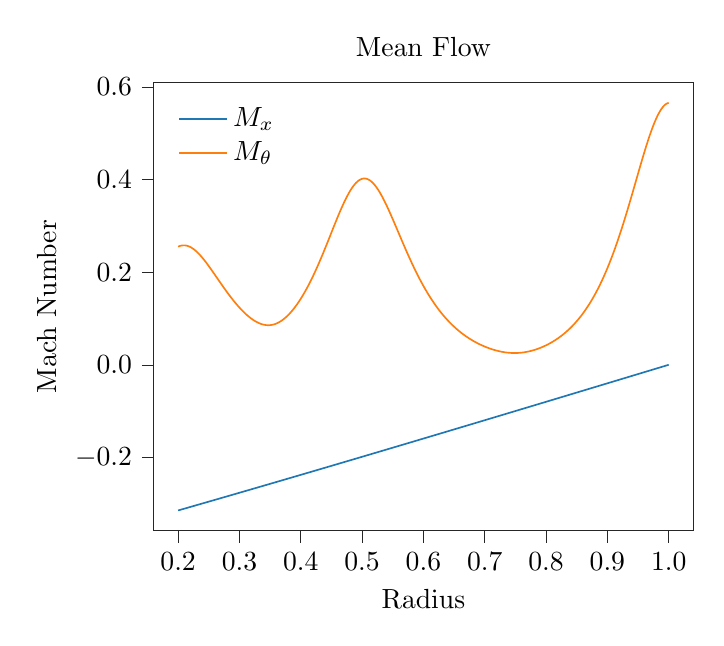
\begin{tikzpicture}

\definecolor{color0}{rgb}{0.12156862745098,0.466666666666667,0.705882352941177}
\definecolor{color1}{rgb}{1,0.498039215686275,0.0549019607843137}

\begin{axis}[
axis line style={white!15!black},
legend cell align={left},
legend style={
  fill opacity=0.8,
  draw opacity=1,
  text opacity=1,
  at={(0.03,0.97)},
  anchor=north west,
  draw=none
},
tick align=outside,
tick pos=left,
title={Mean Flow },
x grid style={white!80!black},
xlabel={Radius},
xmin=0.16, xmax=1.04,
xtick style={color=white!15!black},
xtick={0.1,0.2,0.3,0.4,0.5,0.6,0.7,0.8,0.9,1,1.1},
xticklabels={0.1,0.2,0.3,0.4,0.5,0.6,0.7,0.8,0.9,1.0,1.1},
y grid style={white!80!black},
ylabel={Mach Number},
ymin=-0.358579171685103, ymax=0.609698172253824,
ytick style={color=white!15!black},
ytick={-0.4,-0.2,0,0.2,0.4,0.6,0.8},
yticklabels={\ensuremath{-}0.4,\ensuremath{-}0.2,0.0,0.2,0.4,0.6,0.8}
]
\addplot [semithick, color0]
table {%
0.2 -0.314566565142425
0.2015625 -0.313973231598063
0.203125 -0.313379775407908
0.2046875 -0.312786196803778
0.20625 -0.31219249601754
0.2078125 -0.311598673281109
0.209375 -0.311004728826447
0.2109375 -0.310410662885563
0.2125 -0.309816475690513
0.2140625 -0.309222167473404
0.215625 -0.308627738466385
0.2171875 -0.308033188901657
0.21875 -0.307438519011464
0.2203125 -0.306843729028101
0.221875 -0.306248819183906
0.2234375 -0.305653789711266
0.225 -0.305058640842615
0.2265625 -0.304463372810433
0.228125 -0.303867985847246
0.2296875 -0.303272480185627
0.23125 -0.302676856058197
0.2328125 -0.302081113697619
0.234375 -0.301485253336607
0.2359375 -0.300889275207918
0.2375 -0.300293179544357
0.2390625 -0.299696966578772
0.240625 -0.29910063654406
0.2421875 -0.298504189673163
0.24375 -0.297907626199066
0.2453125 -0.297310946354804
0.246875 -0.296714150373453
0.2484375 -0.296117238488138
0.25 -0.295520210932026
0.2515625 -0.294923067938333
0.253125 -0.294325809740317
0.2546875 -0.293728436571281
0.25625 -0.293130948664575
0.2578125 -0.292533346253593
0.259375 -0.291935629571772
0.2609375 -0.291337798852597
0.2625 -0.290739854329594
0.2640625 -0.290141796236336
0.265625 -0.289543624806439
0.2671875 -0.288945340273564
0.26875 -0.288346942871416
0.2703125 -0.287748432833744
0.271875 -0.28714981039434
0.2734375 -0.286551075787042
0.275 -0.28595222924573
0.2765625 -0.285353271004329
0.278125 -0.284754201296807
0.2796875 -0.284155020357175
0.28125 -0.283555728419489
0.2828125 -0.282956325717846
0.284375 -0.282356812486389
0.2859375 -0.281757188959303
0.2875 -0.281157455370815
0.2890625 -0.280557611955196
0.290625 -0.27995765894676
0.2921875 -0.279357596579864
0.29375 -0.278757425088908
0.2953125 -0.278157144708332
0.296875 -0.277556755672622
0.2984375 -0.276956258216305
0.3 -0.27635565257395
0.3015625 -0.275754938980168
0.303125 -0.275154117669613
0.3046875 -0.274553188876981
0.30625 -0.273952152837011
0.3078125 -0.273351009784481
0.309375 -0.272749759954213
0.3109375 -0.27214840358107
0.3125 -0.271546940899957
0.3140625 -0.270945372145821
0.315625 -0.27034369755365
0.3171875 -0.269741917358471
0.31875 -0.269140031795357
0.3203125 -0.268538041099418
0.321875 -0.267935945505807
0.3234375 -0.267333745249717
0.325 -0.266731440566383
0.3265625 -0.266129031691081
0.328125 -0.265526518859126
0.3296875 -0.264923902305875
0.33125 -0.264321182266725
0.3328125 -0.263718358977114
0.334375 -0.263115432672518
0.3359375 -0.262512403588457
0.3375 -0.261909271960489
0.3390625 -0.261306038024212
0.340625 -0.260702702015264
0.3421875 -0.260099264169323
0.34375 -0.259495724722107
0.3453125 -0.258892083909374
0.346875 -0.258288341966921
0.3484375 -0.257684499130585
0.35 -0.257080555636242
0.3515625 -0.256476511719807
0.353125 -0.255872367617234
0.3546875 -0.255268123564519
0.35625 -0.254663779797693
0.3578125 -0.254059336552828
0.359375 -0.253454794066035
0.3609375 -0.252850152573463
0.3625 -0.252245412311301
0.3640625 -0.251640573515775
0.365625 -0.25103563642315
0.3671875 -0.25043060126973
0.36875 -0.249825468291857
0.3703125 -0.249220237725911
0.371875 -0.248614909808309
0.3734375 -0.248009484775508
0.375 -0.247403962864003
0.3765625 -0.246798344310325
0.378125 -0.246192629351044
0.3796875 -0.245586818222767
0.38125 -0.24498091116214
0.3828125 -0.244374908405845
0.384375 -0.243768810190601
0.3859375 -0.243162616753166
0.3875 -0.242556328330334
0.3890625 -0.241949945158937
0.390625 -0.241343467475843
0.3921875 -0.240736895517956
0.39375 -0.240130229522221
0.3953125 -0.239523469725615
0.396875 -0.238916616365153
0.3984375 -0.238309669677889
0.4 -0.23770262990091
0.4015625 -0.237095497271341
0.403125 -0.236488272026345
0.4046875 -0.235880954403117
0.40625 -0.235273544638891
0.4078125 -0.234666042970938
0.409375 -0.234058449636562
0.4109375 -0.233450764873104
0.4125 -0.232842988917941
0.4140625 -0.232235122008486
0.415625 -0.231627164382187
0.4171875 -0.231019116276527
0.41875 -0.230410977929025
0.4203125 -0.229802749577234
0.421875 -0.229194431458745
0.4234375 -0.228586023811182
0.425 -0.227977526872203
0.4265625 -0.227368940879503
0.428125 -0.226760266070811
0.4296875 -0.22615150268389
0.43125 -0.225542650956538
0.4328125 -0.224933711126589
0.434375 -0.224324683431909
0.4359375 -0.2237155681104
0.4375 -0.223106365399997
0.4390625 -0.222497075538671
0.440625 -0.221887698764424
0.4421875 -0.221278235315296
0.44375 -0.220668685429357
0.4453125 -0.220059049344713
0.446875 -0.219449327299504
0.4484375 -0.218839519531901
0.45 -0.21822962628011
0.4515625 -0.217619647782373
0.453125 -0.21700958427696
0.4546875 -0.21639943600218
0.45625 -0.215789203196369
0.4578125 -0.215178886097901
0.459375 -0.214568484945182
0.4609375 -0.213957999976648
0.4625 -0.21334743143077
0.4640625 -0.212736779546052
0.465625 -0.21212604456103
0.4671875 -0.211515226714272
0.46875 -0.210904326244379
0.4703125 -0.210293343389984
0.471875 -0.209682278389752
0.4734375 -0.209071131482379
0.475 -0.208459902906597
0.4765625 -0.207848592901165
0.478125 -0.207237201704876
0.4796875 -0.206625729556556
0.48125 -0.206014176695061
0.4828125 -0.205402543359278
0.484375 -0.204790829788126
0.4859375 -0.204179036220557
0.4875 -0.203567162895553
0.4890625 -0.202955210052125
0.490625 -0.202343177929319
0.4921875 -0.201731066766209
0.49375 -0.201118876801901
0.4953125 -0.200506608275533
0.496875 -0.19989426142627
0.4984375 -0.199281836493312
0.5 -0.198669333715887
0.5015625 -0.198056753333254
0.503125 -0.197444095584701
0.5046875 -0.196831360709549
0.50625 -0.196218548947147
0.5078125 -0.195605660536874
0.509375 -0.194992695718141
0.5109375 -0.194379654730386
0.5125 -0.193766537813078
0.5140625 -0.193153345205717
0.515625 -0.19254007714783
0.5171875 -0.191926733878976
0.51875 -0.191313315638742
0.5203125 -0.190699822666745
0.521875 -0.190086255202629
0.5234375 -0.18947261348607
0.525 -0.188858897756771
0.5265625 -0.188245108254466
0.528125 -0.187631245218915
0.5296875 -0.18701730888991
0.53125 -0.186403299507269
0.5328125 -0.185789217310838
0.534375 -0.185175062540495
0.5359375 -0.184560835436144
0.5375 -0.183946536237716
0.5390625 -0.183332165185173
0.540625 -0.182717722518503
0.5421875 -0.182103208477722
0.54375 -0.181488623302877
0.5453125 -0.180873967234038
0.546875 -0.180259240511305
0.5484375 -0.179644443374807
0.55 -0.179029576064698
0.5515625 -0.178414638821162
0.553125 -0.177799631884408
0.5546875 -0.177184555494672
0.55625 -0.17656940989222
0.5578125 -0.175954195317341
0.559375 -0.175338912010356
0.5609375 -0.174723560211609
0.5625 -0.17410814016147
0.5640625 -0.17349265210034
0.565625 -0.172877096268643
0.5671875 -0.17226147290683
0.56875 -0.17164578225538
0.5703125 -0.171030024554796
0.571875 -0.170414200045609
0.5734375 -0.169798308968375
0.575 -0.169182351563677
0.5765625 -0.168566328072123
0.578125 -0.167950238734347
0.5796875 -0.16733408379101
0.58125 -0.166717863482796
0.5828125 -0.166101578050417
0.584375 -0.165485227734609
0.5859375 -0.164868812776134
0.5875 -0.164252333415779
0.5890625 -0.163635789894357
0.590625 -0.163019182452705
0.5921875 -0.162402511331685
0.59375 -0.161785776772184
0.5953125 -0.161168979015113
0.596875 -0.160552118301411
0.5984375 -0.159935194872038
0.6 -0.159318208967979
0.6015625 -0.158701160830245
0.603125 -0.158084050699871
0.6046875 -0.157466878817914
0.60625 -0.156849645425458
0.6078125 -0.156232350763609
0.609375 -0.155614995073498
0.6109375 -0.154997578596281
0.6125 -0.154380101573134
0.6140625 -0.15376256424526
0.615625 -0.153144966853885
0.6171875 -0.152527309640257
0.61875 -0.151909592845649
0.6203125 -0.151291816711356
0.621875 -0.150673981478698
0.6234375 -0.150056087389016
0.625 -0.149438134683675
0.6265625 -0.148820123604062
0.628125 -0.14820205439159
0.6296875 -0.147583927287689
0.63125 -0.146965742533818
0.6328125 -0.146347500371453
0.634375 -0.145729201042096
0.6359375 -0.14511084478727
0.6375 -0.144492431848521
0.6390625 -0.143873962467415
0.640625 -0.143255436885543
0.6421875 -0.142636855344516
0.64375 -0.142018218085968
0.6453125 -0.141399525351553
0.646875 -0.140780777382949
0.6484375 -0.140161974421854
0.65 -0.139543116709988
0.6515625 -0.138924204489092
0.653125 -0.138305238000929
0.6546875 -0.137686217487282
0.65625 -0.137067143189957
0.6578125 -0.136448015350779
0.659375 -0.135828834211595
0.6609375 -0.135209600014273
0.6625 -0.134590313000702
0.6640625 -0.133970973412789
0.665625 -0.133351581492465
0.6671875 -0.13273213748168
0.66875 -0.132112641622403
0.6703125 -0.131493094156626
0.671875 -0.13087349532636
0.6734375 -0.130253845373634
0.675 -0.1296341445405
0.6765625 -0.129014393069028
0.678125 -0.12839459120131
0.6796875 -0.127774739179454
0.68125 -0.127154837245591
0.6828125 -0.12653488564187
0.684375 -0.125914884610459
0.6859375 -0.125294834393547
0.6875 -0.12467473523334
0.6890625 -0.124054587372064
0.690625 -0.123434391051966
0.6921875 -0.122814146515309
0.69375 -0.122193854004376
0.6953125 -0.121573513761469
0.696875 -0.120953126028908
0.6984375 -0.120332691049032
0.7 -0.1197122090642
0.7015625 -0.119091680316785
0.703125 -0.118471105049183
0.7046875 -0.117850483503806
0.70625 -0.117229815923084
0.7078125 -0.116609102549465
0.709375 -0.115988343625415
0.7109375 -0.115367539393419
0.7125 -0.114746690095978
0.7140625 -0.114125795975612
0.715625 -0.113504857274856
0.7171875 -0.112883874236266
0.71875 -0.112262847102412
0.7203125 -0.111641776115884
0.721875 -0.111020661519287
0.7234375 -0.110399503555244
0.725 -0.109778302466396
0.7265625 -0.109157058495398
0.728125 -0.108535771884924
0.7296875 -0.107914442877665
0.73125 -0.107293071716326
0.7328125 -0.106671658643631
0.734375 -0.10605020390232
0.7359375 -0.105428707735148
0.7375 -0.104807170384887
0.7390625 -0.104185592094326
0.740625 -0.103563973106267
0.7421875 -0.102942313663532
0.74375 -0.102320614008955
0.7453125 -0.101698874385389
0.746875 -0.1010770950357
0.7484375 -0.100455276202771
0.75 -0.0998334181294999
0.7515625 -0.0992115210587998
0.753125 -0.0985895852335994
0.7546875 -0.0979676108968424
0.75625 -0.0973455982914874
0.7578125 -0.0967235476605083
0.759375 -0.0961014592468934
0.7609375 -0.0954793332936462
0.7625 -0.0948571700437845
0.7640625 -0.0942349697403408
0.765625 -0.0936127326263622
0.7671875 -0.0929904589449099
0.76875 -0.0923681489390598
0.7703125 -0.0917458028519016
0.771875 -0.0911234209265392
0.7734375 -0.0905010034060907
0.775 -0.0898785505336877
0.7765625 -0.0892560625524761
0.778125 -0.0886335397056152
0.7796875 -0.0880109822362778
0.78125 -0.0873883903876507
0.7828125 -0.0867657644029336
0.784375 -0.0861431045253399
0.7859375 -0.0855204109980961
0.7875 -0.0848976840644419
0.7890625 -0.0842749239676299
0.790625 -0.0836521309509258
0.7921875 -0.0830293052576081
0.79375 -0.0824064471309682
0.7953125 -0.0817835568143099
0.796875 -0.0811606345509499
0.7984375 -0.0805376805842171
0.8 -0.0799146951574529
0.8015625 -0.079291678514011
0.803125 -0.0786686308972572
0.8046875 -0.0780455525505696
0.80625 -0.0774224437173381
0.8078125 -0.0767993046409646
0.809375 -0.0761761355648628
0.8109375 -0.0755529367324582
0.8125 -0.0749297083871877
0.8140625 -0.0743064507724999
0.815625 -0.0736831641318549
0.8171875 -0.073059848708724
0.81875 -0.0724365047465898
0.8203125 -0.071813132488946
0.821875 -0.0711897321792973
0.8234375 -0.0705663040611597
0.825 -0.0699428483780596
0.8265625 -0.0693193653735343
0.828125 -0.0686958552911321
0.8296875 -0.0680723183744114
0.83125 -0.0674487548669416
0.8328125 -0.0668251650123019
0.834375 -0.0662015490540821
0.8359375 -0.0655779072358824
0.8375 -0.0649542398013126
0.8390625 -0.0643305469939931
0.840625 -0.0637068290575537
0.8421875 -0.0630830862356343
0.84375 -0.0624593187718844
0.8453125 -0.0618355269099631
0.846875 -0.0612117108935392
0.8484375 -0.0605878709662909
0.85 -0.0599640073719054
0.8515625 -0.0593401203540797
0.853125 -0.0587162101565195
0.8546875 -0.0580922770229398
0.85625 -0.0574683211970645
0.8578125 -0.0568443429226261
0.859375 -0.0562203424433665
0.8609375 -0.0555963200030356
0.8625 -0.0549722758453923
0.8640625 -0.0543482102142038
0.865625 -0.0537241233532457
0.8671875 -0.0531000155063021
0.86875 -0.0524758869171648
0.8703125 -0.0518517378296344
0.871875 -0.0512275684875189
0.8734375 -0.0506033791346345
0.875 -0.0499791700148053
0.8765625 -0.0493549413718627
0.878125 -0.0487306934496463
0.8796875 -0.0481064264920028
0.88125 -0.0474821407427864
0.8828125 -0.0468578364458589
0.884375 -0.0462335138450891
0.8859375 -0.045609173184353
0.8875 -0.0449848147075337
0.8890625 -0.0443604386585211
0.890625 -0.0437360452812123
0.8921875 -0.0431116348195108
0.89375 -0.042487207517327
0.8953125 -0.0418627636185779
0.896875 -0.0412383033671867
0.8984375 -0.0406138270070833
0.9 -0.0399893347822038
0.9015625 -0.0393648269364904
0.903125 -0.0387403037138917
0.9046875 -0.0381157653583617
0.90625 -0.037491212113861
0.9078125 -0.0368666442243555
0.909375 -0.0362420619338172
0.9109375 -0.0356174654862236
0.9125 -0.0349928551255574
0.9140625 -0.0343682310958073
0.915625 -0.0337435936409669
0.9171875 -0.0331189430050354
0.91875 -0.0324942794320168
0.9203125 -0.0318696031659202
0.921875 -0.03124491445076
0.9234375 -0.0306202135305551
0.925 -0.0299955006493293
0.9265625 -0.0293707760511112
0.928125 -0.0287460399799336
0.9296875 -0.0281212926798342
0.93125 -0.0274965343948549
0.9328125 -0.0268717653690419
0.934375 -0.0262469858464456
0.9359375 -0.0256221960711204
0.9375 -0.024997396287125
0.9390625 -0.0243725867385215
0.940625 -0.0237477676693765
0.9421875 -0.0231229393237598
0.94375 -0.0224981019457448
0.9453125 -0.0218732557794089
0.946875 -0.0212484010688324
0.9484375 -0.0206235380580993
0.95 -0.0199986669912967
0.9515625 -0.0193737881125147
0.953125 -0.0187489016658469
0.9546875 -0.0181240078953893
0.95625 -0.0174991070452412
0.9578125 -0.0168741993595044
0.959375 -0.0162492850822834
0.9609375 -0.0156243644576856
0.9625 -0.0149994377298203
0.9640625 -0.0143745051427998
0.965625 -0.0137495669407382
0.9671875 -0.0131246233677519
0.96875 -0.0124996746679598
0.9703125 -0.0118747210854821
0.971875 -0.0112497628644416
0.9734375 -0.0106248002489625
0.975 -0.00999983348317079
0.9765625 -0.00937486281119418
0.978125 -0.00874988847716171
0.9796875 -0.00812491072520414
0.98125 -0.00749992979945334
0.9828125 -0.00687494594404237
0.984375 -0.00624995940310574
0.9859375 -0.00562497042077864
0.9875 -0.00499997924119756
0.9890625 -0.0043749861084996
0.990625 -0.00374999126682261
0.9921875 -0.00312499496030536
0.99375 -0.00249999743308688
0.9953125 -0.00187499892930699
0.996875 -0.00124999969310565
0.9984375 -0.000624999968623085
1 0
};
\addlegendentry{$M_{x}$}
\addplot [semithick, color1]
table {%
0.2 0.255065159843046
0.2015625 0.255968364411969
0.203125 0.256706833358219
0.2046875 0.257279572376127
0.20625 0.257686110072619
0.2078125 0.257926497257104
0.209375 0.258001302302394
0.2109375 0.257911602675627
0.2125 0.257658972790116
0.2140625 0.257245468377284
0.215625 0.256673607621338
0.2171875 0.255946349337276
0.21875 0.255067068504603
0.2203125 0.254039529494257
0.221875 0.25286785734447
0.2234375 0.251556507452602
0.225 0.250110234054432
0.2265625 0.248534057860345
0.228125 0.246833233209701
0.2296875 0.245013215091013
0.23125 0.243079626357068
0.2328125 0.241038225441498
0.234375 0.238894874857357
0.2359375 0.236655510729794
0.2375 0.234326113584628
0.2390625 0.231912680583411
0.240625 0.229421199363994
0.2421875 0.226857623614387
0.24375 0.224227850477382
0.2453125 0.221537699854474
0.246875 0.218792895650435
0.2484375 0.21599904897482
0.25 0.21316164329395
0.2515625 0.210286021506594
0.253125 0.207377374898871
0.2546875 0.204440733918698
0.25625 0.201480960697466
0.2578125 0.198502743236421
0.259375 0.19551059116732
0.2609375 0.192508832991191
0.2625 0.189501614695225
0.2640625 0.186492899645885
0.265625 0.183486469655856
0.2671875 0.180485927123467
0.26875 0.177494698145321
0.2703125 0.174516036506022
0.271875 0.171553028452757
0.2734375 0.168608598167034
0.275 0.165685513850817
0.2765625 0.162786394349561
0.278125 0.159913716240034
0.2796875 0.157069821316225
0.28125 0.154256924411978
0.2828125 0.151477121504055
0.284375 0.148732398044197
0.2859375 0.146024637473106
0.2875 0.143355629873271
0.2890625 0.140727080720902
0.290625 0.138140619700031
0.2921875 0.13559780954393
0.29375 0.133100154870287
0.2953125 0.130649110977115
0.296875 0.128246092566015
0.2984375 0.125892482358112
0.3 0.123589639565741
0.3015625 0.121338908179735
0.303125 0.119141625027891
0.3046875 0.116999127554962
0.30625 0.114912761268305
0.3078125 0.112883886786253
0.309375 0.110913886418458
0.3109375 0.109004170199123
0.3125 0.107156181285485
0.3140625 0.105371400625434
0.315625 0.103651350790409
0.3171875 0.1019975988631
0.31875 0.100411758264908
0.3203125 0.0988954894063168
0.321875 0.0974504990452432
0.3234375 0.0960785382451227
0.325 0.0947813988368702
0.3265625 0.0935609083079101
0.328125 0.0924189230679663
0.3296875 0.0913573200756757
0.33125 0.0903779868524443
0.3328125 0.089482809959776
0.334375 0.0886736620724435
0.3359375 0.0879523878403873
0.3375 0.0873207887944687
0.3390625 0.0867806076117272
0.340625 0.0863335121106115
0.3421875 0.085981079391489
0.34375 0.085724780568301
0.3453125 0.0855659665497199
0.346875 0.0855058553197153
0.3484375 0.0855455211364491
0.35 0.0856858860149973
0.3515625 0.0859277137854266
0.353125 0.0862716069268763
0.3546875 0.0867180062757169
0.35625 0.0872671935977731
0.3578125 0.0879192969077789
0.359375 0.0886742983202184
0.3609375 0.089532044130272
0.3625 0.0904922567562133
0.3640625 0.0915545481281322
0.365625 0.0927184340833403
0.3671875 0.0939833493256452
0.36875 0.0953486625217281
0.3703125 0.0968136911400023
0.371875 0.0983777156816692
0.3734375 0.100039993006174
0.375 0.101799768509913
0.3765625 0.103656286974313
0.378125 0.105608801954347
0.3796875 0.107656583628954
0.38125 0.109798925079123
0.3828125 0.112035146996802
0.384375 0.11436460085794
0.3859375 0.116786670616132
0.3875 0.1193007729899
0.3890625 0.121906356427498
0.390625 0.124602898838949
0.3921875 0.127389904186897
0.39375 0.130266898026433
0.3953125 0.133233422080402
0.396875 0.136289027931298
0.3984375 0.139433269904513
0.4 0.142665697210859
0.4015625 0.145985845409386
0.403125 0.149393227244884
0.4046875 0.152887322908421
0.40625 0.156467569763883
0.4078125 0.160133351579076
0.409375 0.163883987296415
0.4109375 0.167718719375798
0.4125 0.171636701740867
0.4140625 0.175636987359539
0.415625 0.179718515490483
0.4171875 0.183880098629044
0.41875 0.188120409189027
0.4203125 0.192437965960647
0.421875 0.196831120389881
0.4234375 0.201298042730311
0.425 0.205836708125276
0.4265625 0.210444882685797
0.428125 0.215120109638081
0.4296875 0.219859695623494
0.43125 0.224660697243575
0.4328125 0.229519907952808
0.434375 0.234433845412387
0.4359375 0.239398739428929
0.4375 0.244410520612798
0.4390625 0.249464809901279
0.440625 0.254556909101945
0.4421875 0.259681792621032
0.44375 0.264834100550136
0.4453125 0.27000813329177
0.446875 0.275197847909978
0.4484375 0.280396856395864
0.45 0.285598426039319
0.4515625 0.290795482096905
0.453125 0.295980612941552
0.4546875 0.301146077871998
0.45625 0.306283817748479
0.4578125 0.31138546860576
0.459375 0.316442378374904
0.4609375 0.32144562682116
0.4625 0.326386048776775
0.4640625 0.331254260714544
0.465625 0.336040690670567
0.4671875 0.340735611483277
0.46875 0.345329177270684
0.4703125 0.349811463019533
0.471875 0.35417250710938
0.4734375 0.358402356542188
0.475 0.362491114595036
0.4765625 0.366428990560886
0.478125 0.370206351191277
0.4796875 0.37381377340661
0.48125 0.377242097795612
0.4828125 0.380482482386889
0.484375 0.383526456143579
0.4859375 0.386365971608016
0.4875 0.388993456108193
0.4890625 0.391401860932495
0.490625 0.393584707884263
0.4921875 0.395536132643813
0.49375 0.397250924392459
0.4953125 0.398724561190988
0.496875 0.399953240653146
0.4984375 0.400933905512442
0.5 0.401664263746783
0.5015625 0.402142802998784
0.503125 0.402368799108529
0.5046875 0.402342318658297
0.50625 0.402064215513529
0.5078125 0.401536121429045
0.509375 0.400760430872516
0.5109375 0.399740280296358
0.5125 0.398479522163042
0.5140625 0.396982694095653
0.515625 0.395254983584066
0.5171875 0.39330218872638
0.51875 0.391130675524381
0.5203125 0.388747332280452
0.521875 0.386159521661241
0.5234375 0.383375031000781
0.525 0.380402021412906
0.5265625 0.37724897627048
0.528125 0.373924649587917
0.5296875 0.370438014814742
0.53125 0.366798214512707
0.5328125 0.363014511348306
0.534375 0.359096240787847
0.5359375 0.355052765834596
0.5375 0.350893434098191
0.5390625 0.346627537436659
0.540625 0.342264274361892
0.5421875 0.337812715351385
0.54375 0.333281771163073
0.5453125 0.328680164206925
0.546875 0.324016402987131
0.5484375 0.319298759592463
0.55 0.314535250180197
0.5515625 0.309733618370758
0.553125 0.304901321446166
0.5546875 0.300045519225358
0.55625 0.295173065473267
0.5578125 0.290290501688204
0.559375 0.285404053103047
0.5609375 0.280519626730042
0.5625 0.275642811276067
0.5640625 0.27077887875488
0.565625 0.265932787624734
0.5671875 0.261109187283532
0.56875 0.256312423759043
0.5703125 0.251546546438397
0.571875 0.246815315688742
0.5734375 0.242122211229442
0.575 0.237470441125182
0.5765625 0.232862951278719
0.578125 0.22830243531152
0.5796875 0.223791344730069
0.58125 0.219331899285021
0.5828125 0.21492609743956
0.584375 0.210575726872192
0.5859375 0.206282374947681
0.5875 0.202047439097858
0.5890625 0.197872137061639
0.590625 0.193757516940619
0.5921875 0.189704467033205
0.59375 0.185713725416266
0.5953125 0.181785889248833
0.596875 0.177921423777413
0.5984375 0.174120671027024
0.6 0.170383858166168
0.6015625 0.166711105537592
0.603125 0.163102434349923
0.6046875 0.159557774028135
0.60625 0.156076969223248
0.6078125 0.152659786483873
0.609375 0.149305920594004
0.6109375 0.146015000583079
0.6125 0.142786595415612
0.6140625 0.139620219368809
0.615625 0.136515337107451
0.6171875 0.13347136846603
0.61875 0.130487692948654
0.6203125 0.12756365395764
0.621875 0.124698562761982
0.6234375 0.121891702217005
0.625 0.119142330246641
0.6265625 0.116449683099675
0.628125 0.113812978391277
0.6296875 0.11123141794095
0.63125 0.108704190417859
0.6328125 0.106230473804262
0.634375 0.103809437687483
0.6359375 0.101440245390631
0.6375 0.0991220559518919
0.6390625 0.0968540259619605
0.640625 0.0946353112688321
0.6421875 0.092465068558833
0.64375 0.0903424568224584
0.6453125 0.088266638713247
0.646875 0.0862367818075993
0.6484375 0.0842520597731427
0.65 0.0823116534529223
0.6515625 0.0804147518724195
0.653125 0.0785605531761026
0.6546875 0.0767482654999489
0.65625 0.074977107786117
0.6578125 0.0732463105456957
0.659375 0.07155511657523
0.6609375 0.0699027816324986
0.6625 0.0682885750768002
0.6640625 0.0667117804788219
0.665625 0.0651716962049498
0.6671875 0.063667635980726
0.66875 0.0621989294379548
0.6703125 0.0607649226497941
0.671875 0.059364978658023
0.6734375 0.0579984779964363
0.675 0.0566648192142266
0.6765625 0.0553634194029264
0.678125 0.0540937147303553
0.6796875 0.0528551609847307
0.68125 0.0516472341318674
0.6828125 0.0504694308880978
0.684375 0.0493212693111629
0.6859375 0.0482022894109793
0.6875 0.0471120537816698
0.6890625 0.0460501482556922
0.690625 0.0450161825803071
0.6921875 0.0440097911157661
0.69375 0.043030633553821
0.6953125 0.0420783956540049
0.696875 0.0411527899940301
0.6984375 0.0402535567291964
0.7 0.0393804643541552
0.7015625 0.0385333104585603
0.703125 0.0377119224661578
0.7046875 0.0369161583445847
0.70625 0.03614590727077
0.7078125 0.0354010902341206
0.709375 0.0346816605569391
0.7109375 0.0339876043086025
0.7125 0.0333189405871274
0.7140625 0.032675721638941
0.715625 0.0320580327850901
0.7171875 0.0314659921199864
0.71875 0.030899749947283
0.7203125 0.0303594879168096
0.721875 0.0298454178271658
0.7234375 0.0293577800605058
0.725 0.028896841619993
0.7265625 0.02846289374629
0.728125 0.0280562490976937
0.7296875 0.0276772384892812
0.73125 0.0273262071995499
0.7328125 0.0270035108686346
0.734375 0.0267095110295417
0.7359375 0.0264445703327243
0.7375 0.0262090475435282
0.7390625 0.0260032924107508
0.740625 0.0258276405213213
0.7421875 0.0256824082697078
0.74375 0.025567888079597
0.7453125 0.0254843440186413
0.746875 0.02543200794361
0.7484375 0.0254110763027492
0.75 0.0254217077045359
0.7515625 0.0254640213381115
0.753125 0.0255380963015776
0.7546875 0.0256439718618399
0.75625 0.0257816486357861
0.7578125 0.0259510906494439
0.759375 0.0261522282015027
0.7609375 0.0263849614319338
0.7625 0.0266491644768043
0.7640625 0.0269446900775945
0.765625 0.0272713745074708
0.7671875 0.0276290426780044
0.76875 0.0280175132966183
0.7703125 0.0284366039568782
0.771875 0.0288861360590011
0.7734375 0.0293659394755854
0.775 0.0298758568960128
0.7765625 0.030415747801474
0.778125 0.0309854920398314
0.7796875 0.0315849929852943
0.78125 0.0322141802813672
0.7828125 0.0328730121767872
0.784375 0.0335614774730271
0.7859375 0.0342795971084747
0.7875 0.0350274254090058
0.7890625 0.0358050510372605
0.790625 0.0366125976742192
0.7921875 0.0374502244665543
0.79375 0.0383181262722576
0.7953125 0.0392165337353146
0.796875 0.040145713218003
0.7984375 0.0411059666168876
0.8 0.0420976310859398
0.8015625 0.0431210786874706
0.803125 0.0441767159889997
0.8046875 0.0452649836215835
0.80625 0.0463863558127949
0.8078125 0.0475413399053534
0.809375 0.0487304758704063
0.8109375 0.0499543358226658
0.8125 0.0512135235430355
0.8140625 0.0525086740128872
0.815625 0.0538404529629672
0.8171875 0.0552095564387755
0.81875 0.0566167103833332
0.8203125 0.0580626702374222
0.821875 0.0595482205566574
0.8234375 0.0610741746441408
0.825 0.062641374196886
0.8265625 0.0642506889637268
0.828125 0.0659030164120159
0.8296875 0.067599281400005
0.83125 0.0693404358514907
0.8328125 0.0711274584289652
0.834375 0.0729613542012303
0.8359375 0.07484315430113
0.8375 0.0767739155687956
0.8390625 0.0787547201755158
0.840625 0.0807866752230513
0.8421875 0.0828709123129645
0.84375 0.0850085870801981
0.8453125 0.0872008786848752
0.846875 0.0894489892559412
0.8484375 0.0917541432799597
0.85 0.0941175869280004
0.8515625 0.0965405873132023
0.853125 0.0990244316711992
0.8546875 0.101570426455177
0.85625 0.104179896336902
0.8578125 0.106854183104609
0.859375 0.109594644448144
0.8609375 0.112402652621281
0.8625 0.115279592970591
0.8640625 0.118226862319719
0.865625 0.121245867197353
0.8671875 0.124338021896614
0.86875 0.127504746353011
0.8703125 0.130747463827489
0.871875 0.134067598380528
0.8734375 0.13746657212265
0.875 0.14094580222606
0.8765625 0.144506697681637
0.878125 0.148150655784842
0.8796875 0.151879058333667
0.88125 0.15569326752118
0.8828125 0.159594621504825
0.884375 0.163584429634248
0.8859375 0.167663967319096
0.8875 0.171834470518073
0.8890625 0.176097129830408
0.890625 0.180453084170948
0.8921875 0.184903414010309
0.89375 0.189449134161866
0.8953125 0.194091186097979
0.896875 0.198830429778696
0.8984375 0.203667634977241
0.9 0.208603472088054
0.9015625 0.213638502404859
0.903125 0.218773167858416
0.9046875 0.22400778020613
0.90625 0.229342509668755
0.9078125 0.234777373012944
0.909375 0.24031222108247
0.9109375 0.245946725785683
0.9125 0.251680366552035
0.9140625 0.25751241627655
0.915625 0.263441926777863
0.9171875 0.269467713802905
0.91875 0.275588341619623
0.9203125 0.281802107248194
0.921875 0.288107024391076
0.9234375 0.294500807132996
0.925 0.300980853493419
0.9265625 0.307544228926396
0.928125 0.314187649875617
0.9296875 0.320907467506142
0.93125 0.327699651748462
0.9328125 0.334559775805034
0.934375 0.341483001284309
0.9359375 0.348464064142019
0.9375 0.355497261624187
0.9390625 0.36257644042046
0.940625 0.369694986249733
0.9421875 0.376845815112347
0.94375 0.384021366453792
0.9453125 0.391213598493737
0.946875 0.398413985980555
0.9484375 0.405613520635077
0.95 0.412802714547513
0.9515625 0.419971606787799
0.953125 0.427109773481643
0.9546875 0.434206341591764
0.95625 0.44125000662576
0.9578125 0.448229054468482
0.959375 0.455131387507252
0.9609375 0.461944555182711
0.9625 0.468655789056426
0.9640625 0.475252042438538
0.965625 0.481720034565212
0.9671875 0.488046299256582
0.96875 0.494217237922058
0.9703125 0.500219176712006
0.971875 0.506038427543904
0.9734375 0.511661352658388
0.975 0.517074432287396
0.9765625 0.522264334944558
0.978125 0.527217989778637
0.9796875 0.531922660365945
0.98125 0.536366019259179
0.9828125 0.540536222559617
0.984375 0.544421983739021
0.9859375 0.548012645908313
0.9875 0.55129825171366
0.9890625 0.554269610038046
0.990625 0.556918358698616
0.9921875 0.559237022357485
0.99375 0.561219064906353
0.9953125 0.562858935642828
0.996875 0.564152108628062
0.9984375 0.565095114699835
1 0.565685565711145
};
\addlegendentry{$M_{\theta}$}
\end{axis}

\end{tikzpicture}

    \end{center}
\end{figure}

\begin{figure}
    \begin{center}
        % This file was created with tikzplotlib v0.9.12.
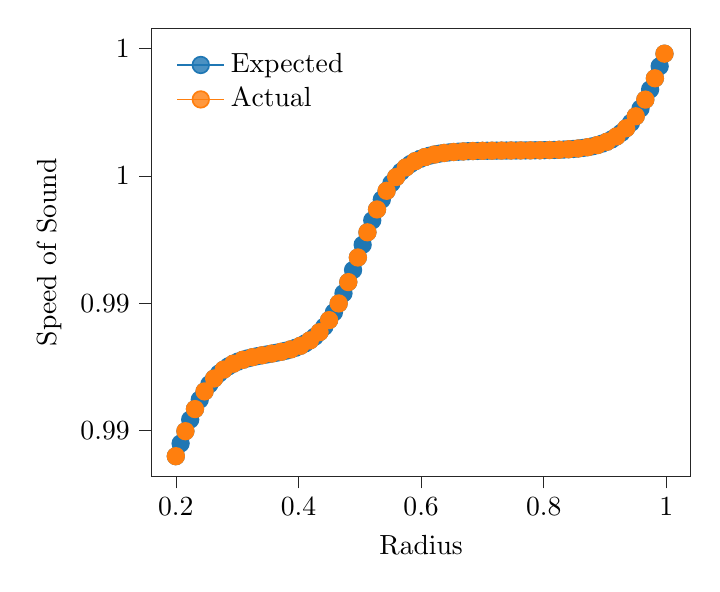
\begin{tikzpicture}

\definecolor{color0}{rgb}{0.12156862745098,0.466666666666667,0.705882352941177}
\definecolor{color1}{rgb}{1,0.498039215686275,0.0549019607843137}

\begin{axis}[
axis line style={white!15!black},
legend cell align={left},
legend style={
  fill opacity=0.8,
  draw opacity=1,
  text opacity=1,
  at={(0.03,0.97)},
  anchor=north west,
  draw=none
},
tick align=outside,
tick pos=left,
x grid style={white!80!black},
xlabel={Radius},
xmin=0.16, xmax=1.04,
xtick style={color=white!15!black},
y grid style={white!80!black},
ylabel={Speed of Sound},
ymin=0.98320056903035, ymax=1.00079997290332,
ytick style={color=white!15!black}
]
\addplot [semithick, color0, mark=*, mark size=3, mark repeat=5, mark options={solid}]
table {%
0.2 0.984000541933667
0.2015625 0.984100548886647
0.203125 0.984200432419622
0.2046875 0.984300068384446
0.20625 0.984399333875707
0.2078125 0.984498107834061
0.209375 0.984596271630271
0.2109375 0.984693709624082
0.2125 0.984790309692462
0.2140625 0.984885963722324
0.215625 0.984980568063398
0.2171875 0.985074023937652
0.21875 0.985166237802302
0.2203125 0.985257121664242
0.221875 0.985346593344428
0.2234375 0.985434576691501
0.225 0.985521001744648
0.2265625 0.985605804846342
0.228125 0.985688928706271
0.2296875 0.985770322418282
0.23125 0.985849941432696
0.2328125 0.985927747486754
0.234375 0.986003708496322
0.2359375 0.986077798412233
0.2375 0.986149997044859
0.2390625 0.986220289860638
0.240625 0.986288667754308
0.2421875 0.986355126800626
0.24375 0.986419667989276
0.2453125 0.986482296946548
0.246875 0.986543023647233
0.2484375 0.986601862119971
0.25 0.986658830149088
0.2515625 0.986713948975696
0.253125 0.98676724300061
0.2546875 0.98681873949133
0.25625 0.986868468295113
0.2578125 0.986916461559873
0.259375 0.986962753464396
0.2609375 0.987007379959106
0.2625 0.987050378518398
0.2640625 0.987091787905317
0.265625 0.987131647949157
0.2671875 0.987169999336396
0.26875 0.98720688341517
0.2703125 0.987242342013376
0.271875 0.987276417270339
0.2734375 0.987309151481869
0.275 0.987340586958444
0.2765625 0.987370765896143
0.278125 0.987399730259926
0.2796875 0.987427521678759
0.28125 0.987454181352077
0.2828125 0.987479749967015
0.284375 0.987504267625839
0.2859375 0.987527773782981
0.2875 0.987550307191088
0.2890625 0.987571905855486
0.290625 0.987592606996474
0.2921875 0.987612447018872
0.29375 0.987631461488276
0.2953125 0.987649685113462
0.296875 0.987667151734442
0.2984375 0.987683894315661
0.3 0.987699944943884
0.3015625 0.987715334830319
0.303125 0.987730094316565
0.3046875 0.987744252883996
0.30625 0.987757839166223
0.3078125 0.987770880964282
0.309375 0.987783405264264
0.3109375 0.987795438257075
0.3125 0.987807005360076
0.3140625 0.987818131240364
0.315625 0.987828839839472
0.3171875 0.987839154399291
0.31875 0.98784909748904
0.3203125 0.987858691033117
0.321875 0.9878679563397
0.3234375 0.987876914129958
0.325 0.987885584567766
0.3265625 0.987893987289837
0.328125 0.98790214143616
0.3296875 0.987910065680699
0.33125 0.987917778262275
0.3328125 0.987925297015572
0.334375 0.987932639402246
0.3359375 0.987939822542074
0.3375 0.987946863244137
0.3390625 0.987953778037998
0.340625 0.987960583204877
0.3421875 0.987967294808789
0.34375 0.98797392872766
0.3453125 0.987980500684408
0.346875 0.987987026277992
0.3484375 0.987993521014427
0.35 0.988000000337782
0.3515625 0.988006479661155
0.353125 0.988012974397646
0.3546875 0.988019499991323
0.35625 0.988026071948201
0.3578125 0.988032705867241
0.359375 0.988039417471358
0.3609375 0.988046222638482
0.3625 0.988053137432628
0.3640625 0.988060178135015
0.365625 0.988067361275209
0.3671875 0.98807470366229
0.36875 0.988082222416037
0.3703125 0.988089934998106
0.371875 0.988097859243185
0.3734375 0.988106013390094
0.375 0.988114416112798
0.3765625 0.988123086551289
0.378125 0.988132044342281
0.3796875 0.988141309649652
0.38125 0.988150903194572
0.3828125 0.98816084628522
0.384375 0.988171160845998
0.3859375 0.988181869446127
0.3875 0.9881929953275
0.3890625 0.988204562431654
0.390625 0.988216595425687
0.3921875 0.988229119726965
0.39375 0.988242161526395
0.3953125 0.988255747810073
0.396875 0.988269906379039
0.3984375 0.988284665866907
0.4 0.988300055755055
0.4015625 0.988316106385087
0.403125 0.988332848968214
0.4046875 0.988350315591207
0.40625 0.988368539218517
0.4078125 0.988387553690159
0.409375 0.988407393714916
0.4109375 0.988428094858389
0.4125 0.988449693525406
0.4140625 0.988472226936272
0.415625 0.988495733096318
0.4171875 0.988520250758199
0.41875 0.988545819376356
0.4203125 0.988572479053063
0.421875 0.988600270475462
0.4234375 0.988629234842998
0.425 0.988659413784646
0.4265625 0.988690849265375
0.428125 0.988723583481276
0.4296875 0.988757658742837
0.43125 0.98879311734588
0.4328125 0.988830001429742
0.434375 0.988868352822332
0.4359375 0.9889082128718
0.4375 0.988949622264638
0.4390625 0.988992620830155
0.440625 0.989037247331411
0.4421875 0.989083539242818
0.44375 0.989131532514817
0.4453125 0.989181261326212
0.446875 0.989232757824935
0.4484375 0.989286051858266
0.45 0.989341170693724
0.4515625 0.989398138732145
0.453125 0.989456977214666
0.4546875 0.989517703925637
0.45625 0.989580332893724
0.4578125 0.989644874093744
0.459375 0.989711333152017
0.4609375 0.989779711058255
0.4625 0.989850003887249
0.4640625 0.989922202533768
0.465625 0.989996292464284
0.4671875 0.990072253489208
0.46875 0.99015005955941
0.4703125 0.990229678590797
0.471875 0.990311072320652
0.4734375 0.99039419619934
0.475 0.990478999320756
0.4765625 0.990565424394636
0.478125 0.990653407763507
0.4796875 0.990742879466609
0.48125 0.99083376335264
0.4828125 0.990925977242617
0.484375 0.991019433143496
0.4859375 0.991114037512562
0.4875 0.991209691571851
0.4890625 0.991306291671168
0.490625 0.991403729697502
0.4921875 0.991501893527903
0.49375 0.991600667522201
0.4953125 0.99169993305125
0.496875 0.991799569055799
0.4984375 0.991899452630537
0.5 0.991999459627421
0.5015625 0.992099465272067
0.503125 0.99219934478671
0.5046875 0.992298974013166
0.50625 0.992398230029186
0.5078125 0.992496991751752
0.509375 0.992595140521059
0.5109375 0.992692560659307
0.5125 0.992789139998857
0.5140625 0.99288477037483
0.515625 0.992979348077864
0.5171875 0.99307277426338
0.51875 0.993164955314424
0.5203125 0.993255803155917
0.521875 0.993345235518834
0.5234375 0.993433176153603
0.525 0.993519554992716
0.5265625 0.993604308263212
0.528125 0.993687378550314
0.5296875 0.993768714814062
0.53125 0.993848272361297
0.5328125 0.993926012775751
0.534375 0.994001903809366
0.5359375 0.99407591923823
0.5375 0.994148038686721
0.5390625 0.99421824742356
0.540625 0.994286536133559
0.5421875 0.994352900668823
0.54375 0.994417341783093
0.5453125 0.994479864852854
0.546875 0.994540479588594
0.5484375 0.994599199739509
0.55 0.994656042794637
0.5515625 0.994711029683234
0.553125 0.994764184476907
0.5546875 0.994815534095789
0.55625 0.994865108020749
0.5578125 0.99491293801338
0.559375 0.99495905784526
0.5609375 0.995003503037712
0.5625 0.995046310613072
0.5640625 0.995087518858254
0.565625 0.995127167101171
0.5671875 0.995165295500434
0.56875 0.99520194484852
0.5703125 0.995237156388507
0.571875 0.995270971644298
0.5734375 0.995303432264168
0.575 0.995334579877347
0.5765625 0.995364455963282
0.578125 0.995393101733155
0.5796875 0.995420558023162
0.58125 0.995446865199025
0.5828125 0.995472063071189
0.584375 0.9954961908201
0.5859375 0.995519286930997
0.5875 0.995541389137587
0.5890625 0.995562534374025
0.590625 0.995582758734604
0.5921875 0.995602097440566
0.59375 0.995620584813474
0.5953125 0.995638254254612
0.596875 0.995655138229866
0.5984375 0.995671268259608
0.6 0.995686674913096
0.6015625 0.995701387806942
0.603125 0.995715435607232
0.6046875 0.995728846034892
0.60625 0.99574164587393
0.6078125 0.995753860982223
0.609375 0.995765516304507
0.6109375 0.995776635887292
0.6125 0.995787242895424
0.6140625 0.995797359630043
0.615625 0.995807007547711
0.6171875 0.995816207280501
0.61875 0.995824978656858
0.6203125 0.995833340723064
0.621875 0.995841311765143
0.6234375 0.995848909331092
0.625 0.995856150253272
0.6265625 0.995863050670899
0.628125 0.995869626052497
0.6296875 0.99587589121825
0.63125 0.995881860362164
0.6328125 0.995887547073985
0.634375 0.995892964360806
0.6359375 0.995898124668321
0.6375 0.995903039901678
0.6390625 0.995907721445908
0.640625 0.995912180185882
0.6421875 0.995916426525794
0.64375 0.995920470408134
0.6453125 0.995924321332153
0.646875 0.995927988371789
0.6484375 0.995931480193072
0.65 0.995934805070983
0.6515625 0.995937970905779
0.653125 0.99594098523878
0.6546875 0.995943855267619
0.65625 0.995946587860976
0.6578125 0.995949189572774
0.659375 0.995951666655872
0.6609375 0.995954025075258
0.6625 0.99595627052074
0.6640625 0.995958408419154
0.665625 0.995960443946116
0.6671875 0.995962382037296
0.66875 0.995964227399259
0.6703125 0.995965984519872
0.671875 0.995967657678284
0.6734375 0.995969250954509
0.675 0.995970768238611
0.6765625 0.995972213239507
0.678125 0.995973589493407
0.6796875 0.995974900371901
0.68125 0.995976149089699
0.6828125 0.995977338712054
0.684375 0.995978472161855
0.6859375 0.995979552226434
0.6875 0.995980581564065
0.6890625 0.995981562710198
0.690625 0.995982498083416
0.6921875 0.995983389991139
0.69375 0.995984240635083
0.6953125 0.995985052116483
0.696875 0.995985826441091
0.6984375 0.99598656552396
0.7 0.995987271194022
0.7015625 0.995987945198473
0.703125 0.995988589206969
0.7046875 0.995989204815643
0.70625 0.995989793550959
0.7078125 0.995990356873398
0.709375 0.995990896180996
0.7109375 0.99599141281273
0.7125 0.99599190805178
0.7140625 0.99599238312864
0.715625 0.995992839224128
0.7171875 0.995993277472259
0.71875 0.995993698963021
0.7203125 0.99599410474504
0.721875 0.99599449582815
0.7234375 0.995994873185871
0.725 0.995995237757798
0.7265625 0.995995590451909
0.728125 0.995995932146805
0.7296875 0.995996263693868
0.73125 0.995996585919359
0.7328125 0.995996899626465
0.734375 0.995997205597271
0.7359375 0.9959975045947
0.7375 0.995997797364393
0.7390625 0.995998084636562
0.740625 0.995998367127788
0.7421875 0.995998645542801
0.74375 0.995998920576223
0.7453125 0.995999192914293
0.746875 0.995999463236562
0.7484375 0.995999732217585
0.75 0.996000000528589
0.7515625 0.996000268839138
0.753125 0.996000537818796
0.7546875 0.996000808138787
0.75625 0.996001080473659
0.7578125 0.996001355502957
0.759375 0.996001633912908
0.7609375 0.996001916398121
0.7625 0.996002203663312
0.7640625 0.996002496425045
0.765625 0.996002795413511
0.7671875 0.996003101374329
0.76875 0.996003415070396
0.7703125 0.996003737283773
0.771875 0.996004068817611
0.7734375 0.996004410498143
0.775 0.996004763176713
0.7765625 0.996005127731883
0.778125 0.996005505071589
0.7796875 0.996005896135382
0.78125 0.996006301896732
0.7828125 0.996006723365422
0.784375 0.996007161590024
0.7859375 0.996007617660467
0.7875 0.996008092710702
0.7890625 0.996008587921481
0.790625 0.996009104523228
0.7921875 0.996009643799046
0.79375 0.996010207087836
0.7953125 0.996010795787547
0.796875 0.996011411358571
0.7984375 0.996012055327279
0.8 0.996012729289704
0.8015625 0.996013434915398
0.803125 0.996014173951444
0.8046875 0.996014948226658
0.80625 0.99601575965597
0.8078125 0.996016610245002
0.809375 0.99601750209485
0.8109375 0.996018437407087
0.8125 0.996019418488979
0.8140625 0.99602044775895
0.815625 0.996021527752279
0.8171875 0.996022661127064
0.81875 0.996023850670446
0.8203125 0.996025099305121
0.821875 0.99602641009613
0.8234375 0.996027786257968
0.825 0.996029231161992
0.8265625 0.996030748344171
0.828125 0.996032341513167
0.8296875 0.996034014558775
0.83125 0.996035771560727
0.8328125 0.996037616797878
0.834375 0.996039554757779
0.8359375 0.996041590146669
0.8375 0.996043727899874
0.8390625 0.996045973192643
0.840625 0.996048331451433
0.8421875 0.996050808365651
0.84375 0.99605340989986
0.8453125 0.996056142306476
0.846875 0.996059012138958
0.8484375 0.99606202626549
0.85 0.996065191883192
0.8515625 0.996068516532841
0.853125 0.996072008114122
0.8546875 0.996075674901416
0.85625 0.996079525560123
0.8578125 0.996083569163517
0.859375 0.996087815210152
0.8609375 0.996092273641784
0.8625 0.996096954861836
0.8640625 0.996101869754369
0.865625 0.996107029703561
0.8671875 0.996112446613664
0.86875 0.99611813292943
0.8703125 0.996124101656964
0.871875 0.996130366384967
0.8734375 0.996136941306354
0.875 0.996143841240155
0.8765625 0.996151081653687
0.878125 0.996158678684891
0.8796875 0.996166649164795
0.88125 0.996175010639986
0.8828125 0.996183781395013
0.884375 0.996192980474604
0.8859375 0.99620262770557
0.8875 0.996212743718267
0.8890625 0.996223349967452
0.890625 0.996234468752366
0.8921875 0.996246123235863
0.89375 0.996258337462352
0.8953125 0.996271136374368
0.896875 0.996284545827466
0.8984375 0.99629859260322
0.9 0.996313304419992
0.9015625 0.996328709941177
0.903125 0.996344838780554
0.9046875 0.996361721504406
0.90625 0.996379389629974
0.9078125 0.996397875619856
0.909375 0.996417212871876
0.9109375 0.996437435703965
0.9125 0.99645857933354
0.9140625 0.996480679850876
0.915625 0.996503774185906
0.9171875 0.996527900067896
0.91875 0.996553095977414
0.9203125 0.996579401090003
0.921875 0.996606855210946
0.9234375 0.996635498700543
0.925 0.996665372389287
0.9265625 0.996696517482366
0.928125 0.996728975452927
0.9296875 0.996762787923574
0.93125 0.996797996535619
0.9328125 0.996834642805644
0.934375 0.99687276796903
0.9359375 0.996912412810164
0.9375 0.996953617479149
0.9390625 0.996996421294959
0.940625 0.997040862535105
0.9421875 0.997086978212043
0.94375 0.997134803836707
0.9453125 0.997184373169752
0.946875 0.997235717961291
0.9484375 0.997288867680121
0.95 0.997343849233688
0.9515625 0.99740068668026
0.953125 0.997459400935069
0.9546875 0.997520009472411
0.95625 0.997582526025983
0.9578125 0.997646960289984
0.959375 0.997713317623768
0.9609375 0.997781598763074
0.9625 0.997851799541075
0.9640625 0.997923910622686
0.965625 0.99799791725571
0.9671875 0.998073799042532
0.96875 0.998151529736121
0.9703125 0.998231077064117
0.971875 0.998312402584702
0.9734375 0.998395461577857
0.975 0.998480202975387
0.9765625 0.998566569332831
0.978125 0.998654496846022
0.9796875 0.998743915414651
0.98125 0.998834748754659
0.9828125 0.998926914560766
0.984375 0.999020324719782
0.9859375 0.99911488557469
0.9875 0.99921049823879
0.9890625 0.999307058958444
0.990625 0.999404459522227
0.9921875 0.999502587713568
0.99375 0.999601327803226
0.9953125 0.999700561077321
0.996875 0.999800166395987
0.9984375 0.999900020777216
1 1
};
\addlegendentry{Expected}
\addplot [semithick, color1, mark=*, mark size=3, mark repeat=10, mark options={solid}]
table {%
0.2 0.984000542019354
0.2015625 0.984100538570465
0.203125 0.984200411755927
0.2046875 0.984300037478986
0.20625 0.984399292884513
0.2078125 0.984498056961819
0.209375 0.984596211128208
0.2109375 0.98469363978739
0.2125 0.984790230857325
0.2140625 0.984885876262573
0.215625 0.98498047238688
0.2171875 0.985073920482345
0.21875 0.985166127032258
0.2203125 0.985257004065404
0.221875 0.985346469420391
0.2234375 0.985434446959279
0.225 0.98552086673049
0.2265625 0.985605665081666
0.228125 0.985688784723747
0.2296875 0.985770174748117
0.23125 0.985849790599148
0.2328125 0.985927594004909
0.234375 0.986003552869154
0.2359375 0.986077641127965
0.2375 0.986149838574637
0.2390625 0.986220130656513
0.240625 0.986288508247539
0.2421875 0.986354967400289
0.24375 0.986419509081172
0.2453125 0.986482138892399
0.246875 0.986542866784147
0.2484375 0.98660170676016
0.25 0.986658676579815
0.2515625 0.986713797459438
0.253125 0.986767093775402
0.2546875 0.986818592771284
0.25625 0.986868324271075
0.2578125 0.98691632040021
0.259375 0.986962615315875
0.2609375 0.987007244947868
0.2625 0.987050246750991
0.2640625 0.987091659469774
0.265625 0.987131522916112
0.2671875 0.987169877760217
0.26875 0.987206765335094
0.2703125 0.987242227454642
0.271875 0.987276306245304
0.2734375 0.987309043991106
0.275 0.987340482991801
0.2765625 0.987370665433774
0.278125 0.987399633273278
0.2796875 0.987427428131517
0.28125 0.987454091201058
0.2828125 0.987479663163019
0.284375 0.987504184114449
0.2859375 0.987527693505313
0.2875 0.98755023008449
0.2890625 0.987571831854191
0.290625 0.9875925360322
0.2921875 0.987612379021383
0.29375 0.987631396385893
0.2953125 0.987649622833532
0.296875 0.987667092203763
0.2984375 0.987683837460875
0.3 0.987699890691827
0.3015625 0.987715283108339
0.303125 0.987730045052807
0.3046875 0.987744206007658
0.30625 0.987757794607782
0.3078125 0.987770838655695
0.309375 0.987783365139148
0.3109375 0.98779540025086
0.3125 0.987806969410141
0.3140625 0.987818097286156
0.315625 0.987828807822605
0.3171875 0.987839124263634
0.31875 0.98784906918079
0.3203125 0.987858664500862
0.321875 0.987867931534466
0.3234375 0.987876891005252
0.325 0.987885563079613
0.3265625 0.987893967396799
0.328125 0.987902123099364
0.3296875 0.987910048863849
0.33125 0.987917762931659
0.3328125 0.987925283140076
0.334375 0.987932626953352
0.3359375 0.987939811493866
0.3375 0.987946853573297
0.3390625 0.987953769723811
0.340625 0.98796057622922
0.3421875 0.987967289156136
0.34375 0.987973924385075
0.3453125 0.987980497641544
0.346875 0.987987024527085
0.3484375 0.987993520550299
0.35 0.988000001157834
0.3515625 0.988006481765371
0.353125 0.98801297778859
0.3546875 0.988019504674139
0.35625 0.988026077930618
0.3578125 0.988032713159569
0.359375 0.988039426086497
0.3609375 0.988046232591919
0.3625 0.988053148742442
0.3640625 0.98806019082188
0.365625 0.988067375362393
0.3671875 0.988074719175661
0.36875 0.988082239384058
0.3703125 0.988089953451836
0.371875 0.988097879216269
0.3734375 0.988106034918762
0.375 0.988114439235851
0.3765625 0.988123111310083
0.378125 0.988132070780705
0.3796875 0.988141337814104
0.38125 0.988150933133922
0.3828125 0.988160878050769
0.384375 0.988171194491426
0.3859375 0.988181905027431
0.3875 0.988193032902921
0.3890625 0.988204602061585
0.390625 0.988216637172577
0.3921875 0.988229163655196
0.39375 0.988242207702146
0.3953125 0.988255796301162
0.396875 0.988269957254748
0.3984375 0.988284719197773
0.4 0.988300111612648
0.4015625 0.988316164841748
0.403125 0.98833291009677
0.4046875 0.988350379464653
0.40625 0.988368605909658
0.4078125 0.988387623271224
0.409375 0.988407466257124
0.4109375 0.988428170431479
0.4125 0.988449772197124
0.4140625 0.988472308771811
0.415625 0.988495818157714
0.4171875 0.988520339103674
0.41875 0.988545911059617
0.4203125 0.988572574122552
0.421875 0.988600368973554
0.4234375 0.988629336805148
0.425 0.988659519238492
0.4265625 0.988690958229793
0.428125 0.988723695965391
0.4296875 0.988757774744993
0.43125 0.988793236852577
0.4328125 0.988830124414544
0.434375 0.988868479244747
0.4359375 0.988908342676152
0.4375 0.988949755378929
0.4390625 0.98899275716494
0.440625 0.989037386778686
0.4421875 0.989083681674941
0.44375 0.989131677783485
0.4453125 0.989181409261496
0.446875 0.989232908234404
0.4484375 0.989286204526211
0.45 0.989341325380513
0.4515625 0.989398295173717
0.453125 0.989457135122194
0.4546875 0.989517862985384
0.45625 0.989580492767111
0.4578125 0.989645034417647
0.459375 0.989711493539319
0.4609375 0.98977987109867
0.4625 0.989850163148432
0.4640625 0.989922360562726
0.465625 0.989996448789093
0.4671875 0.990072407621048
0.46875 0.990150210994911
0.4703125 0.990229826814696
0.471875 0.990311216808754
0.4734375 0.990394336421754
0.475 0.990479134745392
0.4765625 0.990565554490936
0.478125 0.990653532006369
0.4796875 0.990742997340459
0.48125 0.99083387435562
0.4828125 0.990926080890818
0.484375 0.991019528975192
0.4859375 0.991114125092381
0.4875 0.991209770494826
0.4890625 0.991306361566602
0.490625 0.991403790232585
0.4921875 0.991501944411025
0.49375 0.991600708505906
0.4953125 0.991699963934777
0.496875 0.991799589687169
0.4984375 0.991899462908144
0.5 0.991999459501105
0.5015625 0.992099454743644
0.503125 0.992199323909957
0.5046875 0.992298942893246
0.50625 0.992398188821544
0.5078125 0.992496940660486
0.509375 0.992595079796797
0.5109375 0.99269249059664
0.5125 0.992789060933354
0.5140625 0.992884682679702
0.515625 0.992979252160325
0.5171875 0.993072670560762
0.51875 0.993164844290118
0.5203125 0.993255685295191
0.521875 0.99334511132459
0.5234375 0.99343304614214
0.525 0.99351941968955
0.5265625 0.993604168199006
0.528125 0.993687234256956
0.5296875 0.993768566820951
0.53125 0.993848121191855
0.5328125 0.993925858944195
0.534375 0.99400174781777
0.5359375 0.994075761573883
0.5375 0.994147879819793
0.5390625 0.994218087805088
0.540625 0.994286376193745
0.5421875 0.99435274081564
0.54375 0.994417182401192
0.5453125 0.994479706302753
0.546875 0.994540322206146
0.5484375 0.99459904383561
0.55 0.994655888655176
0.5515625 0.994710877569247
0.553125 0.994764034624923
0.5546875 0.994815386718341
0.55625 0.994864963307029
0.5578125 0.994912796130018
0.559375 0.994958918937205
0.5609375 0.995003367229198
0.5625 0.995046178008647
0.5640625 0.995087389543851
0.565625 0.995127041145225
0.5671875 0.995165172955
0.56875 0.99520182575041
0.5703125 0.995237040760414
0.571875 0.995270859495909
0.5734375 0.995303323593251
0.575 0.995334474670805
0.5765625 0.995364354198178
0.578125 0.995393003377691
0.5796875 0.995420463037613
0.58125 0.995446773536632
0.5828125 0.995471974678994
0.584375 0.995496105639743
0.5859375 0.99551920489945
0.5875 0.99554131018785
0.5890625 0.995562458435763
0.590625 0.995582685734742
0.5921875 0.995602027303832
0.59375 0.995620517462904
0.5953125 0.995638189612002
0.596875 0.99565507621619
0.5984375 0.99567120879539
0.6 0.99568661791875
0.6015625 0.995701333203077
0.603125 0.995715383314918
0.6046875 0.995728795975899
0.60625 0.995741597970942
0.6078125 0.995753815159019
0.609375 0.995765472486118
0.6109375 0.995776594000141
0.6125 0.995787202867441
0.6140625 0.995797321390759
0.615625 0.995806971028341
0.6171875 0.995816172414004
0.61875 0.995824945377991
0.6203125 0.995833308968413
0.621875 0.995841281473156
0.6234375 0.995848880442084
0.625 0.995856122709439
0.6265625 0.995863024416314
0.628125 0.995869601033097
0.6296875 0.995875867381824
0.63125 0.995881837658331
0.6328125 0.995887525454166
0.634375 0.995892943778198
0.6359375 0.995898105077859
0.6375 0.995903021260004
0.6390625 0.995907703711326
0.640625 0.995912163318324
0.6421875 0.995916410486774
0.64375 0.995920455160706
0.6453125 0.995924306840866
0.646875 0.995927974602643
0.6484375 0.995931467113475
0.65 0.995934792649703
0.6515625 0.9959379591129
0.653125 0.995940974045658
0.6546875 0.995943844646839
0.65625 0.995946577786306
0.6578125 0.995949180019123
0.659375 0.99595165759925
0.6609375 0.995954016492733
0.6625 0.995956262390396
0.6640625 0.995958400720057
0.665625 0.995960436658271
0.6671875 0.99596237514161
0.66875 0.995964220877508
0.6703125 0.995965978354663
0.671875 0.995967651853024
0.6734375 0.99596924545337
0.675 0.995970763046498
0.6765625 0.99597220834203
0.678125 0.995973584876848
0.6796875 0.995974896023187
0.68125 0.995976144996378
0.6828125 0.995977334862262
0.684375 0.995978468544298
0.6859375 0.995979548830358
0.6875 0.995980578379236
0.6890625 0.995981559726879
0.690625 0.995982495292344
0.6921875 0.995983387383507
0.69375 0.995984238202519
0.6953125 0.995985049851032
0.696875 0.995985824335194
0.6984375 0.995986563570442
0.7 0.995987269386074
0.7015625 0.995987943529633
0.703125 0.995988587671111
0.7046875 0.995989203406963
0.70625 0.99598979226396
0.7078125 0.995990355702877
0.709375 0.995990895122031
0.7109375 0.995991411860674
0.7125 0.995991907202242
0.7140625 0.995992382377482
0.715625 0.99599283856745
0.7171875 0.995993276906392
0.71875 0.99599369848452
0.7203125 0.995994104350672
0.721875 0.99599449551489
0.7234375 0.995994872950893
0.725 0.995995237598466
0.7265625 0.995995590365778
0.728125 0.995995932131606
0.7296875 0.995996263747507
0.73125 0.995996586039915
0.7328125 0.995996899812179
0.734375 0.995997205846547
0.7359375 0.995997504906098
0.7375 0.995997797736628
0.7390625 0.995998085068498
0.740625 0.995998367618437
0.7421875 0.995998646091321
0.74375 0.995998921181916
0.7453125 0.995999193576601
0.746875 0.99599946395507
0.7484375 0.995999732992015
0.75 0.996000001358802
0.7515625 0.996000269725134
0.753125 0.996000538760714
0.7546875 0.996000809136904
0.75625 0.996001081528391
0.7578125 0.99600135661486
0.759375 0.99600163508268
0.7609375 0.996001917626605
0.7625 0.996002204951495
0.7640625 0.996002497774063
0.765625 0.996002796824648
0.7671875 0.996003102849025
0.76875 0.996003416610248
0.7703125 0.996003738890537
0.771875 0.996004070493211
0.7734375 0.99600441224467
0.775 0.996004764996435
0.7765625 0.996005129627247
0.778125 0.996005507045229
0.7796875 0.996005898190124
0.78125 0.996006304035602
0.7828125 0.996006725591651
0.784375 0.996007163907057
0.7859375 0.996007620071971
0.7875 0.996008095220578
0.7890625 0.996008590533865
0.790625 0.99600910724251
0.7921875 0.996009646629875
0.79375 0.99601021003513
0.7953125 0.996010798856509
0.796875 0.996011414554698
0.7984375 0.996012058656374
0.8 0.996012732757891
0.8015625 0.996013438529137
0.803125 0.996014177717544
0.8046875 0.996014952152294
0.80625 0.996015763748697
0.8078125 0.996016614512774
0.809375 0.996017506546037
0.8109375 0.996018442050494
0.8125 0.996019423333868
0.8140625 0.996020452815054
0.815625 0.996021533029831
0.8171875 0.996022666636814
0.81875 0.996023856423687
0.8203125 0.996025105313711
0.821875 0.996026416372521
0.8234375 0.996027792815226
0.825 0.996029238013831
0.8265625 0.996030755504977
0.828125 0.99603234899803
0.8296875 0.996034022383518
0.83125 0.996035779741937
0.8328125 0.996037625352941
0.834375 0.996039563704913
0.8359375 0.996041599504958
0.8375 0.996043737689303
0.8390625 0.99604598343414
0.840625 0.996048342166902
0.8421875 0.996050819578012
0.84375 0.996053421633092
0.8453125 0.996056154585657
0.846875 0.996059024990304
0.8484375 0.996062039716402
0.85 0.996065205962296
0.8515625 0.996068531270032
0.853125 0.996072023540612
0.8546875 0.996075691049775
0.85625 0.996079542464325
0.8578125 0.996083586858985
0.859375 0.996087833733802
0.8609375 0.996092293032069
0.8625 0.996096975158789
0.8640625 0.996101890999645
0.865625 0.996107051940475
0.8671875 0.996112469887234
0.86875 0.996118157286407
0.8703125 0.996124127145869
0.871875 0.99613039305612
0.8734375 0.996136969211897
0.875 0.996143870434077
0.8765625 0.996151112191834
0.878125 0.996158710624979
0.8796875 0.996166682566409
0.88125 0.996175045564575
0.8828125 0.996183817905873
0.884375 0.996193018636852
0.8859375 0.996202667586109
0.8875 0.996212785385732
0.8890625 0.996223393492147
0.890625 0.996234514206185
0.8921875 0.996246170692186
0.89375 0.996258386995937
0.8953125 0.996271188061206
0.896875 0.996284599744623
0.8984375 0.996298648828654
0.9 0.996313363032339
0.9015625 0.996328771019508
0.903125 0.99634490240411
0.9046875 0.996361787752286
0.90625 0.996379458580801
0.9078125 0.996397947351397
0.909375 0.996417287460625
0.9109375 0.996437513224683
0.9125 0.996458659858756
0.9140625 0.996480763450336
0.915625 0.996503860925981
0.9171875 0.996527990010936
0.91875 0.996553189181057
0.9203125 0.996579497606432
0.921875 0.996606955086097
0.9234375 0.996635601973261
0.925 0.996665479090439
0.9265625 0.9966966276339
0.928125 0.996729089066892
0.9296875 0.9967629050011
0.93125 0.996798117065855
0.9328125 0.996834766764676
0.934375 0.996872895318767
0.9359375 0.996912543497216
0.9375 0.996953751433694
0.9390625 0.996996558429622
0.940625 0.997041002743852
0.9421875 0.997087121369108
0.94375 0.997134949795571
0.9453125 0.997184521762187
0.946875 0.997235868996483
0.9484375 0.997289020943902
0.95 0.997344004487888
0.9515625 0.997400843662211
0.953125 0.997459559357272
0.9546875 0.997520169022392
0.95625 0.997582686366363
0.9578125 0.997647121058781
0.959375 0.997713478434953
0.9609375 0.997781759207394
0.9625 0.997851959187171
0.9640625 0.997924069018498
0.965625 0.997998073930204
0.9671875 0.998073953507733
0.96875 0.998151681489463
0.9703125 0.998231225591102
0.971875 0.99831254736186
0.9734375 0.998395602075987
0.975 0.998480338663054
0.9765625 0.998566699680098
0.978125 0.998654621328378
0.9796875 0.998744033517082
0.98125 0.998834859975838
0.9828125 0.998927018417289
0.984375 0.999020420750399
0.9859375 0.999114973344484
0.9875 0.999210577343224
0.9890625 0.999307129027227
0.990625 0.999404520222934
0.9921875 0.999502638754955
0.99375 0.999601368938184
0.9953125 0.999700592105417
0.996875 0.999800187165552
0.9984375 0.999900031186939
1 1
};
\addlegendentry{Actual}
\end{axis}

\end{tikzpicture}

    \end{center}
\end{figure}

\begin{figure}
    \begin{center}
        % This file was created with tikzplotlib v0.9.12.
\begin{tikzpicture}

\definecolor{color0}{rgb}{0.12156862745098,0.466666666666667,0.705882352941177}

\begin{groupplot}[group style={group size=1 by 2}]
\nextgroupplot[
axis line style={white!15!black},
legend cell align={left},
legend style={fill opacity=0.8, draw opacity=1, text opacity=1, draw=none},
log basis y={10},
scaled x ticks=manual:{}{\pgfmathparse{#1}},
tick align=outside,
tick pos=left,
title={Rate Of Convergence},
x grid style={white!80!black},
xmin=0.49602339181245, xmax=0.60495126705655,
xtick style={color=white!15!black},
xticklabels={},
y grid style={white!80!black},
ymin=1.93465772282466, ymax=2.50490389113768,
ymode=log,
ytick style={color=white!15!black}
]
\addplot [semithick, color0]
table {%
0.6 2.220755792495
0.555555555556 2.163324274032
0.529411764706 2.475663773488
0.515151515152 1.957508006467
0.507692307692 1.997639457419
0.503875968992 1.996551880759
0.501945525292 1.997726606828
0.500974658869 1.998727064418
};
\addlegendentry{Speed Of Sound}

\nextgroupplot[
axis line style={white!15!black},
legend cell align={left},
legend style={fill opacity=0.8, draw opacity=1, text opacity=1, draw=none},
log basis y={10},
tick align=outside,
tick pos=left,
x grid style={white!80!black},
xlabel={Del r},
xmin=0.49602339181245, xmax=0.60495126705655,
xtick style={color=white!15!black},
y grid style={white!80!black},
ymin=0.362953235346687, ymax=0.506191289267272,
ymode=log,
ytick style={color=white!15!black}
]
\addplot [semithick, color0]
table {%
0.6 0.368482797082
0.555555555556 0.423998453276
0.529411764706 0.458768919907
0.515151515152 0.478465639055
0.507692307692 0.488986846835
0.503875968992 0.494429721197
0.501945525292 0.497198646885
0.500974658869 0.498595233207
};
\addlegendentry{LEE}
\end{groupplot}

\end{tikzpicture}

    \end{center}
\end{figure}

\begin{figure}
    \begin{center}
        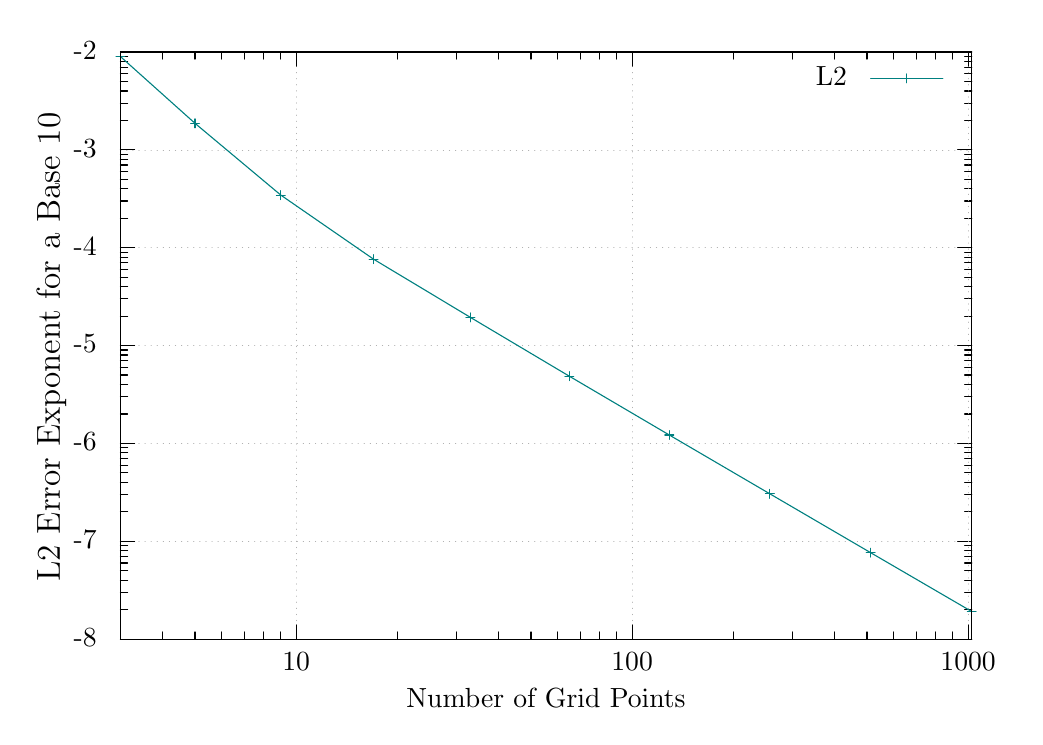
\begin{tikzpicture}[gnuplot]
%% generated with GNUPLOT 5.2p8 (Lua 5.3; terminal rev. Nov 2018, script rev. 108)
%% Tue 21 Sep 2021 05:01:33 PM EDT
\path (0.000,0.000) rectangle (12.500,8.750);
\gpcolor{color=gp lt color axes}
\gpsetlinetype{gp lt axes}
\gpsetdashtype{gp dt axes}
\gpsetlinewidth{0.50}
\draw[gp path] (1.136,0.985)--(11.947,0.985);
\gpcolor{color=gp lt color border}
\gpsetlinetype{gp lt border}
\gpsetdashtype{gp dt solid}
\gpsetlinewidth{1.00}
\draw[gp path] (1.136,0.985)--(1.316,0.985);
\draw[gp path] (11.947,0.985)--(11.767,0.985);
\node[gp node right] at (0.952,0.985) {{-8}};
\draw[gp path] (1.136,1.359)--(1.226,1.359);
\draw[gp path] (11.947,1.359)--(11.857,1.359);
\draw[gp path] (1.136,1.578)--(1.226,1.578);
\draw[gp path] (11.947,1.578)--(11.857,1.578);
\draw[gp path] (1.136,1.733)--(1.226,1.733);
\draw[gp path] (11.947,1.733)--(11.857,1.733);
\draw[gp path] (1.136,1.854)--(1.226,1.854);
\draw[gp path] (11.947,1.854)--(11.857,1.854);
\draw[gp path] (1.136,1.952)--(1.226,1.952);
\draw[gp path] (11.947,1.952)--(11.857,1.952);
\draw[gp path] (1.136,2.035)--(1.226,2.035);
\draw[gp path] (11.947,2.035)--(11.857,2.035);
\draw[gp path] (1.136,2.107)--(1.226,2.107);
\draw[gp path] (11.947,2.107)--(11.857,2.107);
\draw[gp path] (1.136,2.171)--(1.226,2.171);
\draw[gp path] (11.947,2.171)--(11.857,2.171);
\gpcolor{color=gp lt color axes}
\gpsetlinetype{gp lt axes}
\gpsetdashtype{gp dt axes}
\gpsetlinewidth{0.50}
\draw[gp path] (1.136,2.228)--(11.947,2.228);
\gpcolor{color=gp lt color border}
\gpsetlinetype{gp lt border}
\gpsetdashtype{gp dt solid}
\gpsetlinewidth{1.00}
\draw[gp path] (1.136,2.228)--(1.316,2.228);
\draw[gp path] (11.947,2.228)--(11.767,2.228);
\node[gp node right] at (0.952,2.228) {{-7}};
\draw[gp path] (1.136,2.602)--(1.226,2.602);
\draw[gp path] (11.947,2.602)--(11.857,2.602);
\draw[gp path] (1.136,2.821)--(1.226,2.821);
\draw[gp path] (11.947,2.821)--(11.857,2.821);
\draw[gp path] (1.136,2.976)--(1.226,2.976);
\draw[gp path] (11.947,2.976)--(11.857,2.976);
\draw[gp path] (1.136,3.096)--(1.226,3.096);
\draw[gp path] (11.947,3.096)--(11.857,3.096);
\draw[gp path] (1.136,3.195)--(1.226,3.195);
\draw[gp path] (11.947,3.195)--(11.857,3.195);
\draw[gp path] (1.136,3.278)--(1.226,3.278);
\draw[gp path] (11.947,3.278)--(11.857,3.278);
\draw[gp path] (1.136,3.350)--(1.226,3.350);
\draw[gp path] (11.947,3.350)--(11.857,3.350);
\draw[gp path] (1.136,3.413)--(1.226,3.413);
\draw[gp path] (11.947,3.413)--(11.857,3.413);
\gpcolor{color=gp lt color axes}
\gpsetlinetype{gp lt axes}
\gpsetdashtype{gp dt axes}
\gpsetlinewidth{0.50}
\draw[gp path] (1.136,3.470)--(11.947,3.470);
\gpcolor{color=gp lt color border}
\gpsetlinetype{gp lt border}
\gpsetdashtype{gp dt solid}
\gpsetlinewidth{1.00}
\draw[gp path] (1.136,3.470)--(1.316,3.470);
\draw[gp path] (11.947,3.470)--(11.767,3.470);
\node[gp node right] at (0.952,3.470) {{-6}};
\draw[gp path] (1.136,3.844)--(1.226,3.844);
\draw[gp path] (11.947,3.844)--(11.857,3.844);
\draw[gp path] (1.136,4.063)--(1.226,4.063);
\draw[gp path] (11.947,4.063)--(11.857,4.063);
\draw[gp path] (1.136,4.218)--(1.226,4.218);
\draw[gp path] (11.947,4.218)--(11.857,4.218);
\draw[gp path] (1.136,4.339)--(1.226,4.339);
\draw[gp path] (11.947,4.339)--(11.857,4.339);
\draw[gp path] (1.136,4.437)--(1.226,4.437);
\draw[gp path] (11.947,4.437)--(11.857,4.437);
\draw[gp path] (1.136,4.521)--(1.226,4.521);
\draw[gp path] (11.947,4.521)--(11.857,4.521);
\draw[gp path] (1.136,4.593)--(1.226,4.593);
\draw[gp path] (11.947,4.593)--(11.857,4.593);
\draw[gp path] (1.136,4.656)--(1.226,4.656);
\draw[gp path] (11.947,4.656)--(11.857,4.656);
\gpcolor{color=gp lt color axes}
\gpsetlinetype{gp lt axes}
\gpsetdashtype{gp dt axes}
\gpsetlinewidth{0.50}
\draw[gp path] (1.136,4.713)--(11.947,4.713);
\gpcolor{color=gp lt color border}
\gpsetlinetype{gp lt border}
\gpsetdashtype{gp dt solid}
\gpsetlinewidth{1.00}
\draw[gp path] (1.136,4.713)--(1.316,4.713);
\draw[gp path] (11.947,4.713)--(11.767,4.713);
\node[gp node right] at (0.952,4.713) {{-5}};
\draw[gp path] (1.136,5.087)--(1.226,5.087);
\draw[gp path] (11.947,5.087)--(11.857,5.087);
\draw[gp path] (1.136,5.306)--(1.226,5.306);
\draw[gp path] (11.947,5.306)--(11.857,5.306);
\draw[gp path] (1.136,5.461)--(1.226,5.461);
\draw[gp path] (11.947,5.461)--(11.857,5.461);
\draw[gp path] (1.136,5.582)--(1.226,5.582);
\draw[gp path] (11.947,5.582)--(11.857,5.582);
\draw[gp path] (1.136,5.680)--(1.226,5.680);
\draw[gp path] (11.947,5.680)--(11.857,5.680);
\draw[gp path] (1.136,5.763)--(1.226,5.763);
\draw[gp path] (11.947,5.763)--(11.857,5.763);
\draw[gp path] (1.136,5.835)--(1.226,5.835);
\draw[gp path] (11.947,5.835)--(11.857,5.835);
\draw[gp path] (1.136,5.899)--(1.226,5.899);
\draw[gp path] (11.947,5.899)--(11.857,5.899);
\gpcolor{color=gp lt color axes}
\gpsetlinetype{gp lt axes}
\gpsetdashtype{gp dt axes}
\gpsetlinewidth{0.50}
\draw[gp path] (1.136,5.956)--(11.947,5.956);
\gpcolor{color=gp lt color border}
\gpsetlinetype{gp lt border}
\gpsetdashtype{gp dt solid}
\gpsetlinewidth{1.00}
\draw[gp path] (1.136,5.956)--(1.316,5.956);
\draw[gp path] (11.947,5.956)--(11.767,5.956);
\node[gp node right] at (0.952,5.956) {{-4}};
\draw[gp path] (1.136,6.330)--(1.226,6.330);
\draw[gp path] (11.947,6.330)--(11.857,6.330);
\draw[gp path] (1.136,6.549)--(1.226,6.549);
\draw[gp path] (11.947,6.549)--(11.857,6.549);
\draw[gp path] (1.136,6.704)--(1.226,6.704);
\draw[gp path] (11.947,6.704)--(11.857,6.704);
\draw[gp path] (1.136,6.824)--(1.226,6.824);
\draw[gp path] (11.947,6.824)--(11.857,6.824);
\draw[gp path] (1.136,6.923)--(1.226,6.923);
\draw[gp path] (11.947,6.923)--(11.857,6.923);
\draw[gp path] (1.136,7.006)--(1.226,7.006);
\draw[gp path] (11.947,7.006)--(11.857,7.006);
\draw[gp path] (1.136,7.078)--(1.226,7.078);
\draw[gp path] (11.947,7.078)--(11.857,7.078);
\draw[gp path] (1.136,7.141)--(1.226,7.141);
\draw[gp path] (11.947,7.141)--(11.857,7.141);
\gpcolor{color=gp lt color axes}
\gpsetlinetype{gp lt axes}
\gpsetdashtype{gp dt axes}
\gpsetlinewidth{0.50}
\draw[gp path] (1.136,7.198)--(11.947,7.198);
\gpcolor{color=gp lt color border}
\gpsetlinetype{gp lt border}
\gpsetdashtype{gp dt solid}
\gpsetlinewidth{1.00}
\draw[gp path] (1.136,7.198)--(1.316,7.198);
\draw[gp path] (11.947,7.198)--(11.767,7.198);
\node[gp node right] at (0.952,7.198) {{-3}};
\draw[gp path] (1.136,7.572)--(1.226,7.572);
\draw[gp path] (11.947,7.572)--(11.857,7.572);
\draw[gp path] (1.136,7.791)--(1.226,7.791);
\draw[gp path] (11.947,7.791)--(11.857,7.791);
\draw[gp path] (1.136,7.946)--(1.226,7.946);
\draw[gp path] (11.947,7.946)--(11.857,7.946);
\draw[gp path] (1.136,8.067)--(1.226,8.067);
\draw[gp path] (11.947,8.067)--(11.857,8.067);
\draw[gp path] (1.136,8.165)--(1.226,8.165);
\draw[gp path] (11.947,8.165)--(11.857,8.165);
\draw[gp path] (1.136,8.249)--(1.226,8.249);
\draw[gp path] (11.947,8.249)--(11.857,8.249);
\draw[gp path] (1.136,8.321)--(1.226,8.321);
\draw[gp path] (11.947,8.321)--(11.857,8.321);
\draw[gp path] (1.136,8.384)--(1.226,8.384);
\draw[gp path] (11.947,8.384)--(11.857,8.384);
\gpcolor{color=gp lt color axes}
\gpsetlinetype{gp lt axes}
\gpsetdashtype{gp dt axes}
\gpsetlinewidth{0.50}
\draw[gp path] (1.136,8.441)--(11.947,8.441);
\gpcolor{color=gp lt color border}
\gpsetlinetype{gp lt border}
\gpsetdashtype{gp dt solid}
\gpsetlinewidth{1.00}
\draw[gp path] (1.136,8.441)--(1.316,8.441);
\draw[gp path] (11.947,8.441)--(11.767,8.441);
\node[gp node right] at (0.952,8.441) {{-2}};
\draw[gp path] (1.136,0.985)--(1.136,1.075);
\draw[gp path] (1.136,8.441)--(1.136,8.351);
\draw[gp path] (1.669,0.985)--(1.669,1.075);
\draw[gp path] (1.669,8.441)--(1.669,8.351);
\draw[gp path] (2.083,0.985)--(2.083,1.075);
\draw[gp path] (2.083,8.441)--(2.083,8.351);
\draw[gp path] (2.421,0.985)--(2.421,1.075);
\draw[gp path] (2.421,8.441)--(2.421,8.351);
\draw[gp path] (2.706,0.985)--(2.706,1.075);
\draw[gp path] (2.706,8.441)--(2.706,8.351);
\draw[gp path] (2.954,0.985)--(2.954,1.075);
\draw[gp path] (2.954,8.441)--(2.954,8.351);
\draw[gp path] (3.172,0.985)--(3.172,1.075);
\draw[gp path] (3.172,8.441)--(3.172,8.351);
\gpcolor{color=gp lt color axes}
\gpsetlinetype{gp lt axes}
\gpsetdashtype{gp dt axes}
\gpsetlinewidth{0.50}
\draw[gp path] (3.367,0.985)--(3.367,8.441);
\gpcolor{color=gp lt color border}
\gpsetlinetype{gp lt border}
\gpsetdashtype{gp dt solid}
\gpsetlinewidth{1.00}
\draw[gp path] (3.367,0.985)--(3.367,1.165);
\draw[gp path] (3.367,8.441)--(3.367,8.261);
\node[gp node center] at (3.367,0.677) {$10$};
\draw[gp path] (4.652,0.985)--(4.652,1.075);
\draw[gp path] (4.652,8.441)--(4.652,8.351);
\draw[gp path] (5.403,0.985)--(5.403,1.075);
\draw[gp path] (5.403,8.441)--(5.403,8.351);
\draw[gp path] (5.936,0.985)--(5.936,1.075);
\draw[gp path] (5.936,8.441)--(5.936,8.351);
\draw[gp path] (6.350,0.985)--(6.350,1.075);
\draw[gp path] (6.350,8.441)--(6.350,8.351);
\draw[gp path] (6.688,0.985)--(6.688,1.075);
\draw[gp path] (6.688,8.441)--(6.688,8.351);
\draw[gp path] (6.973,0.985)--(6.973,1.075);
\draw[gp path] (6.973,8.441)--(6.973,8.351);
\draw[gp path] (7.221,0.985)--(7.221,1.075);
\draw[gp path] (7.221,8.441)--(7.221,8.351);
\draw[gp path] (7.439,0.985)--(7.439,1.075);
\draw[gp path] (7.439,8.441)--(7.439,8.351);
\gpcolor{color=gp lt color axes}
\gpsetlinetype{gp lt axes}
\gpsetdashtype{gp dt axes}
\gpsetlinewidth{0.50}
\draw[gp path] (7.634,0.985)--(7.634,8.441);
\gpcolor{color=gp lt color border}
\gpsetlinetype{gp lt border}
\gpsetdashtype{gp dt solid}
\gpsetlinewidth{1.00}
\draw[gp path] (7.634,0.985)--(7.634,1.165);
\draw[gp path] (7.634,8.441)--(7.634,8.261);
\node[gp node center] at (7.634,0.677) {$100$};
\draw[gp path] (8.919,0.985)--(8.919,1.075);
\draw[gp path] (8.919,8.441)--(8.919,8.351);
\draw[gp path] (9.670,0.985)--(9.670,1.075);
\draw[gp path] (9.670,8.441)--(9.670,8.351);
\draw[gp path] (10.203,0.985)--(10.203,1.075);
\draw[gp path] (10.203,8.441)--(10.203,8.351);
\draw[gp path] (10.617,0.985)--(10.617,1.075);
\draw[gp path] (10.617,8.441)--(10.617,8.351);
\draw[gp path] (10.955,0.985)--(10.955,1.075);
\draw[gp path] (10.955,8.441)--(10.955,8.351);
\draw[gp path] (11.240,0.985)--(11.240,1.075);
\draw[gp path] (11.240,8.441)--(11.240,8.351);
\draw[gp path] (11.488,0.985)--(11.488,1.075);
\draw[gp path] (11.488,8.441)--(11.488,8.351);
\draw[gp path] (11.706,0.985)--(11.706,1.075);
\draw[gp path] (11.706,8.441)--(11.706,8.351);
\gpcolor{color=gp lt color axes}
\gpsetlinetype{gp lt axes}
\gpsetdashtype{gp dt axes}
\gpsetlinewidth{0.50}
\draw[gp path] (11.901,0.985)--(11.901,8.441);
\gpcolor{color=gp lt color border}
\gpsetlinetype{gp lt border}
\gpsetdashtype{gp dt solid}
\gpsetlinewidth{1.00}
\draw[gp path] (11.901,0.985)--(11.901,1.165);
\draw[gp path] (11.901,8.441)--(11.901,8.261);
\node[gp node center] at (11.901,0.677) {$1000$};
\draw[gp path] (1.136,8.441)--(1.136,0.985)--(11.947,0.985)--(11.947,8.441)--cycle;
\node[gp node center,rotate=-270,font={\fontsize{12.0pt}{14.4pt}\selectfont}] at (0.292,4.713) {L2 Error Exponent for a Base 10};
\node[gp node center] at (6.541,0.215) {Number of Grid Points};
\node[gp node right] at (10.479,8.107) {L2};
\gpcolor{rgb color={0.000,0.502,0.502}}
\draw[gp path] (10.663,8.107)--(11.579,8.107);
\draw[gp path] (1.136,8.383)--(2.083,7.535)--(3.172,6.624)--(4.350,5.810)--(5.580,5.071)%
  --(6.836,4.324)--(8.106,3.577)--(9.383,2.830)--(10.664,2.082)--(11.947,1.335);
\gpsetpointsize{4.00}
\gppoint{gp mark 1}{(1.136,8.383)}
\gppoint{gp mark 1}{(2.083,7.535)}
\gppoint{gp mark 1}{(3.172,6.624)}
\gppoint{gp mark 1}{(4.350,5.810)}
\gppoint{gp mark 1}{(5.580,5.071)}
\gppoint{gp mark 1}{(6.836,4.324)}
\gppoint{gp mark 1}{(8.106,3.577)}
\gppoint{gp mark 1}{(9.383,2.830)}
\gppoint{gp mark 1}{(10.664,2.082)}
\gppoint{gp mark 1}{(11.947,1.335)}
\gppoint{gp mark 1}{(11.121,8.107)}
\gpcolor{color=gp lt color border}
\draw[gp path] (1.136,8.441)--(1.136,0.985)--(11.947,0.985)--(11.947,8.441)--cycle;
%% coordinates of the plot area
\gpdefrectangularnode{gp plot 1}{\pgfpoint{1.136cm}{0.985cm}}{\pgfpoint{11.947cm}{8.441cm}}
\end{tikzpicture}
%% gnuplot variables

    \end{center}
\end{figure}


% % \begin{figure}[h!]
%     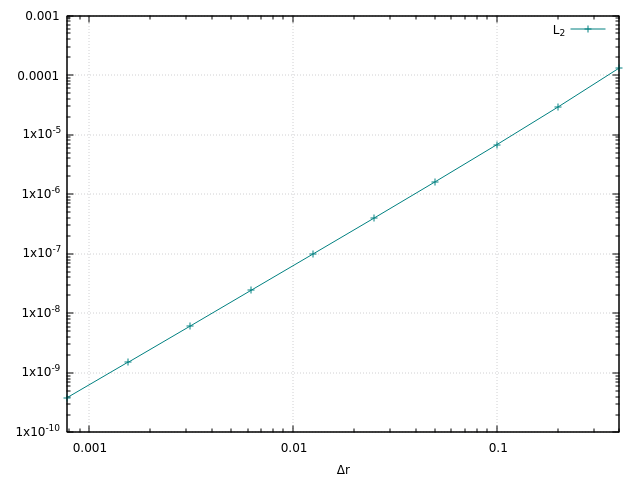
\includegraphics[width=\textwidth]{Figures/l2vDr}
% \end{figure}


% \begin{figure}[h]
%     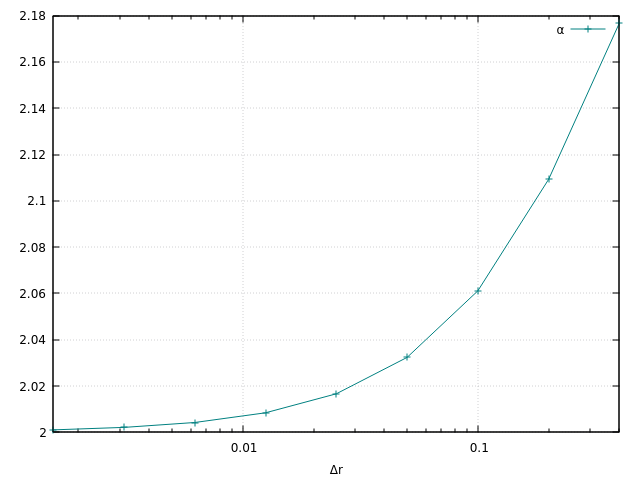
\includegraphics[width=\textwidth]{Figures/alphaVdr}
% \end{figure}


\section{Conclusion}
\section{Appendix}

\subsection{Error Analysis}


Reference: A. Ralston, A first course in numerical analysis 2nd edition

\subsubsection{Exact Polynomial Approximation}


Say we have some discrete data,

\begin{equation*}
    \left( x_{i},y_2 \right),\left( x_2, y_2 \right), \dots , \left( x_n,y_n \right)
\end{equation*}
We want to find a polynomial of the LEAST degree that gits these points exactly. 
Such a polynomial is called a Lagrange Polynomial. If in addition you supply a
function, or derivative value, you can use Hermitie intepolation to help the 
desired fitted polynomial handle sudden changes (?)

For Lagrange Polynomials, the general form is,

\begin{equation*}
    p\left( x_i  \right) =
    \sum_{j=1}^{n} l_j(x_i) f(x_j) + \underbrace{\frac{f^{(n)}\left( c \right)}
    {n!}p_n(x_i)}_{\text{Error at } x_i},
\end{equation*}
where,

\begin{equation*}
    p_n(x_i) = \prod_{j = 1}^{n} \left( x_i - x_j \right) 
\end{equation*}

\begin{equation*}
    p_n(x_i) =  \left( x_{i} - x_{j} \right) 
    \left( x_i - x_{i+1} \right)
    \left( x_i - x_{i+2} \right)
    \left( x_i - x_{i+3} \right) \dots
    ( x_i - x_n)
\end{equation*}

So if we have two data points $x_i$ and $x_{i+1}$, the function of least degree
that fits the data \textit{exactly} for a Langrange interpolation is,

\begin{equation*}
    p(x_i) = l_{i}(x_i)f(x_{i}) + l_{i+1}(x_{i+1})f(x_{i+1}) + \left[\text{
        Error at $x_i$}
    \right]
\end{equation*}

Note that I said \textit{exactly}! So I will drop the error term\dots

Then we \textit{claim} that

\begin{align*}
    p(x_i) =  
    l_i\left( x_i\right)f_i\left( x_i\right) + 
    l_{i+1}\left( x_{i+1}\right)f_{i+1}\left( x_{i+1}\right) 
\end{align*}

which means that we also claim that
\begin{align*}
    l_i(x) = \frac{x - x_{i+1}}{x_{i} - x_{i+1}} \\
    l_{i+1}(x) = \frac{x - x_{i}}{x_{i+1} - x_{i}}
\end{align*}

if $x = x_i$,
\[ l_i(x_i) = \frac{x_i - x_{i+1}}{x_i - x_{i+1} }= 1\], 
\[l_{i + 1}(x_i) = \frac{x_i-x_i}{x_{i+1} - x_{i}} = 0\]
and 
if $x = x_{i+1}$,

\[ l_i(x_{i+1}) = \frac{x_{i+1} - x_{i+1}}{x_i - x_{i+1} }= 0\], 
\[l_{i + 1}(x_{i+1}) = \frac{x_{i+1}-x_i}{x_{i+1} - x_{i}} = 1\]

let's see if $p\left( x \right)$ passes through these points exactly,

\begin{align*}
    p\left( x_i \right) &= 1 f_i(x_i) + 0 f\left( x_i  \right) =  f\left( x_i  \right) \\
    p\left( x_{i+1} \right) &= 1 f_{i+1}(x_{i+1}) + 0 f\left( x_{i+1}  \right) =  f\left( x_{i+1}  \right) 
\end{align*}

Defining,

\begin{align*}
    \Delta x^+ &= x_{i+1} - x_i \\
    \hat{x} &= x - x_i 
\end{align*}
Using this on the Lagrange polynomial for two points gives 

\begin{align*}
    \left( \frac{
            \left( x - x_{i+1} \right)
            }{
            \left( x_i - x_{i+1} \right)
        }
        f_i
        + \frac{
            \left( x - x_i  \right)
            }{
            \left(x_{i+1}- x_i \right)
        }
        f_{i+1}
    \right) \\
    \left( 
        \frac{
            \left( x - \left( x_{i+1} \right) \right)
            }{
            \left( x_i - x_{i+1}\right)
        } 
        f_i + 
        \frac{
            \left( x + \left( -x_i \right) \right)
            }{
            \left( \left( x_{i+1} \right) + \left( -x_i \right) \right)
        }
        f_{i+1}
    \right) \\
    \left(
        \frac{
            (x-\left( \Delta x^+ + x_i \right)) 
            }{
            x_i - (\Delta x^+ + x_i)
        }
        f_i
        +
        \frac{ 
            \left( x + \left( \hat{x} - x \right) \right)
            }{
            \left( \left( \Delta x^+ + x_i \right) + \left( -x_i \right) \right)
        }
        f_{i+1}
    \right)  \\
    \left(
        \frac{
            (\left(x-x_i  \right) -\Delta x^+)   
            }{ 
            - \Delta x^+ 
        }
        f_i
        +
        \frac{
            \left(   \hat{x}    \right)
            }{\left( \left(  \Delta x^+ + x_i \right)  + \left( -x_i \right) \right)
        } f_{i+1}
    \right) \\
    \frac{
        \hat{x} - \Delta x^+
        }{
        -\Delta x^+
    }
    f_i
    +
    \frac{
        \hat{x}
        }{
        \Delta x^+
    }
    f_{i+1}
\end{align*}

The Lagrange polynomial is

\begin{equation*}
    \widetilde{f}\left( \hat{x} \right) 
    =
    \left( 
        \frac{\hat{x}}{\Delta x^+}f_{i+1} +
        \frac{\Delta x^+ - \hat{x}}{\Delta x^+}f_i
    \right)
\end{equation*}

\subsection{Integration}

Recall that 

\[ \hat{x} = x - x_i\]
Now we prepare to integrate,

\begin{align*}
    \int_{x_1}^{x_2} \widetilde{f} dx &=
    \int_{x_1-x_i}^{x_2-x_i} \widetilde{f} \frac{\partial x}{\partial \hat{x}}d\hat{x}\\
                                      &=
                                      \int_{x_1-x_i}^{x_2 - x_i} \widetilde{f} d\hat{x}
\end{align*}

In the interior of the domain $i = 1, iMax - 1$, the function is integrated 
from $\hat{x} = 0$ to $\hat{x} = \Delta x^+$. In other words ,the integration 
covers the complete range of the polynomial. Note that we are only integrating
over a single interval.

\begin{align*}
    \int_0^{\Delta x^+} \widetilde{f} d\hat{x}&=
    \int_0^{\Delta x^+}
    \left( 
        \frac{\hat{x}}{\Delta x^+}f_{i+1} +
        \frac{\Delta x^+ - \hat{x}}{\Delta x^+}f_i
\right) \\ &= 
\frac{1}{\Delta x^+}f_{i+1}
\int_{0}^{\Delta x^+} 
\left(\hat{x}  \right) d\hat{x}
+
\frac{1}{\Delta x^+}
f_{i}
\left(
    \int_{0}^{\Delta x^+} 
    \left( \Delta x^+  \right) d\hat{x}
    -
    \int_{0}^{\Delta x^+} 
    \left( 
        \hat{x}
    \right) d\hat{x}
\right)\\
           &=\frac{1}{\Delta x^+}
           \left( 
               f_{i+1}\left[ 
                   \frac{\left( \Delta x^+ \right)^2}{
                   2} - 0
               \right]_0^{\Delta x^+}
               +
               f_i
               \left[ 
\frac{\left( \Delta x^+ \right)^2}{
                   2} - 0
               \right]_0^{\Delta x^+}
           \right) \\ &=
           \frac{\left( \Delta x^+ \right)^2}{2 \Delta x^+}
           \left[ f_{i+1} +f_i\right] \\
           &= 
           \frac{\Delta x^+}{2 }
           \left[ f_{i+1} +f_i\right] 
\end{align*}
Which is the trapezoidal rule!
\subsection{Taylor Series Error Analysis}

Here we try to determine the order of accuracy of the trapezoidal rule. 
The Taylor series for the integral $F$ and for the function $f$ are:

\begin{align*}
    f_{i+1} &= f_i +
    \Delta x \frac{\partial f}{\partial x}|_i +
    \frac{\Delta x^2}{2} \frac{\partial^2 f}{\partial x^2}|_i +
    \mathcal{O}\left( \Delta x^3 \right) \\
    f_i &= f_i
\end{align*}
Summing the two gives,

\begin{align*}
f_i + f_{i+1} = 2 f_i  + \Delta x \frac{\partial f}{\partial x } +
\mathcal{O}\left( \Delta x^2 \right) 
\end{align*}
Multiplying by $\Delta x /2  $

\begin{align*}
    \frac{\Delta x}{2 }(f_i + f_{i+1} )= 
    f_i {\Delta x} + \frac{\Delta x ^2}{2}\frac{\partial f}{\partial x } +
\mathcal{O}\left( \Delta x^3 \right) 
\end{align*}


\subsection{Composie Trapezoidal Rule}
To account for the entire domain, we express our trapezoidal rule as the sum 
of sub intervals for a uniform grid, to do so we redefine the grid spacing,

\[\Delta x^+   = \frac{\Delta \widetilde{ x}^+  }{n - 1}   \]

where $\widetilde{x}+$ is the length of the domain
and $n$ is the total number of grid points. 

\begin{align*}
    \int_{x_1}^{x_n} \widetilde{f} d \hat{x} &= 
    \frac{\Delta x^+}{2} \sum_{i=1}^{n}
    \left( 
        f_i + f_{i+1}
    \right) \\ 
    &=
    \frac{\Delta x^+}{2}  
    \left[ 
        \left( f_1 + f_2 \right) +
        \left( f_2 + f_3 \right)  +\dots +
        \left( f_{n-2} + f_{n-1} \right) + 
        \left( f_{n-1} + f_{n} \right)  
    \right] \\
    &=
    \frac{\Delta x^+}{2}  
    \left[ 
        \left( f_1 +
            2f_2  +
         2f_3+\dots +
         2f_{n-2} + 
         2f_{n-1}  + 
         f_{n} \right)  
    \right] \\
    &=
    \frac{\Delta x^+}{2}
    \left[ 
        f_1 + f_n + 
        2 \sum_{i=2}^{n-1}
        f_i
    \right] \\
    &=
    \frac{\Delta x^+}{2}
    \left[ 
        f_1 + f_n \right] 
        + 
        \Delta x^+ \sum_{i=2}^{n-1}
    f_i
\end{align*}

Noe we can use A taylor series expansion on the composite trapezoidal rule to
get an order of accuracy

the summation will be expanded Around $ i \Delta x$ in order to interpret the sum 
as a Riemann sum
\begin{align*}
    f_1  &= f_1\\
    i\Delta x \frac{\partial f }{\partial x } +
    \frac{(i\Delta x)^2}{2!} \frac{\partial^2 f }{\partial x^2 } +
    \frac{(i\Delta x)^3}{3!} \frac{\partial^3 f }{\partial x^3 } + \dots
\end{align*}

Let's further simplify the Taylor series at the last grid point,
\begin{align*} 
    f_n &= f_1 + 
    \Delta \widetilde{x}^+\frac{\partial f }{\partial x  } +
    \frac{(\Delta \widetilde{x}^+)^2}{2!}\frac{\partial^2 f }{\partial x^2  } +
    \frac{(\Delta \widetilde{x}^+)^3}{3!}\frac{\partial^3 f }{\partial x^3  } + \dots \\
        &= 
        f_1 +
        \left( n - 1 \right)\Delta x^+ 
        \frac{\partial f}{\partial x} +
        \frac{\left( n - 1 \right)^2}{2}\Delta x^+ 
        \frac{\partial^2 f}{\partial x^2} +
        \frac{\left( n - 1 \right)^3}{3}\Delta x^+ 
        \frac{\partial^3 f}{\partial x^3}
\end{align*}

Okay this is a bit tricky, lets distribute the summation on the Taylor series 
expanded around each grid point. Since this Taylor Series expanison involves 
the 1st grid point we re-adjust our summation to show this.

\begin{align*}
    \sum_{i = 2}^{n - 1} f_i  &= 
    \sum_{i = 1}^{n - 2} \left( 
    f_1 +
    i\Delta x \frac{\partial f }{\partial x } +
    \frac{(i\Delta x)^2}{2!} \frac{\partial^2 f }{\partial x^2 } +
    \frac{(i\Delta x)^3}{3!} \frac{\partial^3 f }{\partial x^3 } + \dots
    \right) \\
                              &=
    \sum_{i = 1}^{n - 2} \left( 
    f_1 \right) +
    \sum_{i = 1}^{n - 2} \left( 
    i\Delta x \frac{\partial f }{\partial x }\right) +
    \sum_{i = 1}^{n - 2} \left( 
    \frac{(i\Delta x)^2}{2!} \frac{\partial^2 f }{\partial x^2 } \right)+
    \sum_{i = 1}^{n - 2} \left( 
    \frac{(i\Delta x)^3}{3!} \frac{\partial^3 f }{\partial x^3 } \right)+ \dots\\ 
                              &=
    \sum_{i = 1}^{n - 2} \left( 
    f_1 \right) +
 \Delta x \frac{\partial f }{\partial x }   
     \sum_{i = 1}^{n - 2} \left( i\right) +
    \frac{(\Delta x)^2}{2!} \frac{\partial^2 f }{\partial x^2 } 
    \sum_{i = 1}^{n - 2} \left( i^2 \right)
    +
    \frac{(\Delta x)^3}{3!} \frac{\partial^3 f }{\partial x^3 } 
    \sum_{i = 1}^{n - 2} \left( i^3 \right)
\end{align*} 
Now we can  substitute this into the composite trapezoial rule and gather the coefficients 


\begin{align*}
    \frac{\Delta x^+ }{2}\left[ f_1 + f_n \right] + \Delta x^+ \sum_{i=1}^{n-2} f_i 
\end{align*}
Let's look at one common term at a time, starting with $f_1$, note the two halfs
summing to one,
\begin{align*} \frac{\Delta x^+}{2}\left[ f_1 + f_1 + \sum_{i=1}^{n-2} f_1 \right] \\
    \Delta x^+ f_1\left[ 1 + \sum_{i=1}^{n-2}1 \right]
\end{align*}

Now for the rest of the terms, we factor out $\Delta x^+$
\begin{align*}
    (\Delta x^+)^2 \frac{\partial f}{\partial x } \left(
        \sum_{i = 1}^{n - 2} \left( i\right) + \frac{n-1}{2} \right) + \\
        \frac{(\Delta x^+)^3}{2!} \frac{\partial^2 f}{\partial x^2 } \left(
    \sum_{i = 1}^{n - 2} \left( i\right)^2 + \frac{(n-1)^2}{2} \right)  + \\
    \frac{(\Delta x^+)^4}{3!} \frac{\partial^3 f}{\partial x^3 } \left(
    \sum_{i = 1}^{n - 2} \left( i\right)^3 + \frac{(n-1)^3}{2} \right) \dots
\end{align*}

Using the following summation rules we can further simplify the problem


\begin{align*}
    \sum_{i = 1}^{n}c= cn  \\
    \sum_{i = 1}^{n}i =  \frac{n\left( n-1\right)}{2}  \\
    \sum_{i = 1}^{n}i^2  = \frac{n^3}{3} + \frac{n^2}{2} + \frac{n}{6}   \\
    \sum_{i = 1}^{n}i^3  = \frac{n^4}{4} + \frac{n^3}{2} + \frac{n^2}{4}  
\end{align*}
Let's put the terms back together, and then simplify with the closed form 
expressions for the summations,
\begin{align*}
    \Delta x^+ f_1\left[ 1 + \sum_{i=1}^{n-2}1 \right] + \\
    (\Delta x^+)^2 \frac{\partial f}{\partial x } \left(
        \sum_{i = 1}^{n - 2} \left( i\right) + \frac{n-1}{2} \right) + \\
        \frac{(\Delta x^+)^3}{2!} \frac{\partial^2 f}{\partial x^2 } \left(
    \sum_{i = 1}^{n - 2} \left( i\right)^2 + \frac{(n-1)^2}{2} \right)  + \\
    \frac{(\Delta x^+)^4}{3!} \frac{\partial^3 f}{\partial x^3 } \left(
    \sum_{i = 1}^{n - 2} \left( i\right)^3 + \frac{(n-1)^3}{2} \right) \dots
\end{align*}

\begin{align*}
    \Delta x^+ f_1\left[ 1 + (n - 2)  \right] + \\
    (\Delta x^+)^2 \frac{\partial f}{\partial x } \left(
    \frac{(n-2)[\left( n-2 \right)-1]}{2} + \frac{n-1}{2} \right) + \\
        \frac{(\Delta x^+)^3}{2!} \frac{\partial^2 f}{\partial x^2 } \left(
        \frac{(n-2)^3}{3} + \frac{(n-2)^2}{2} + \frac{(n-2)}{6} + \frac{(n-1)^2}{2} \right)  + \\
    \frac{(\Delta x^+)^4}{3!} \frac{\partial^3 f}{\partial x^3 } \left(
    \frac{(n-2)^4}{4} + \frac{(n-2)^3}{2} + \frac{(n-2)^2}{4} + \frac{(n-1)^3}{2} \right) \dots
\end{align*}

\begin{align*}
    \Delta x^+ f_1\left[ (n - 1)  \right] + \\
    (\Delta x^+)^2 \frac{\partial f}{\partial x } \left(
    \frac{(n-2)\left( n-1 \right)}{2} + \frac{n-1}{2} \right) + \\
        \frac{(\Delta x^+)^3}{2!} \frac{\partial^2 f}{\partial x^2 } \left(
        \frac{(n-2)^3}{3} + \frac{(n-2)^2}{2} + \frac{(n-2)}{6} + \frac{(n-1)^2}{2} \right)  + \\
    \frac{(\Delta x^+)^4}{3!} \frac{\partial^3 f}{\partial x^3 } \left(
    \frac{(n-2)^4}{4} + \frac{(n-2)^3}{2} + \frac{(n-2)^2}{4} + \frac{(n-1)^3}{2} \right) \dots
\end{align*}

\begin{align*}
     f_1\left[ \Delta \widetilde{x}^+  \right] + \\
    (\Delta x^+)^2 \frac{\partial f}{\partial x } \left(
    \frac{(n-2)\left( n-1 \right)}{2} + \frac{n-1}{2} \right) + \\
        \frac{(\Delta x^+)^3}{2!} \frac{\partial^2 f}{\partial x^2 } \left(
        \frac{(n-2)^3}{3} + \frac{(n-2)^2}{2} + \frac{(n-2)}{6} + \frac{(n-1)^2}{2} \right)  + 
\end{align*}

Side note: 

\begin{align*}
    \frac{(n - 2)(n-1)}{2} + \frac{(n-1)}{2}\\
    \frac{(n - 2)(n-1) + (n-1)}{2} 
\end{align*}
Factor out $(n-1)$
\begin{align*}
    \frac{\left[ \left( n - 2 \right) + 1 \left( n - 1 \right) \right]}{2} \\
    \frac{\left( n-1 \right)\left( n - 1 \right)}{2} \\
    \frac{\left( n - 1 \right)^2}{2}
\end{align*}

Using this for the coefficient of the second term,

\begin{align*}
     f_1\left[ \Delta \widetilde{x}^+  \right] + \\
    (\Delta x^+)^2 \frac{\partial f}{\partial x } \left(
    \frac{(n-1)^2}{2}  \right) + \\
        \frac{(\Delta x^+)^3}{2!} \frac{\partial^2 f}{\partial x^2 } \left(
        \frac{(n-2)^3}{3} + \frac{(n-2)^2}{2} + \frac{(n-2)}{6} + \frac{(n-1)^2}{2} \right)  +
\end{align*}

Since we expect the third term to have a $\left( n-1 \right)^3$ if this pattern
of the Taylor series being expanded around L, the coefficient of the third term
is going to be set equal to $\left( n-1 \right)^3$ and simplified,

We also expect the leading coeffient to have 1/6 as well. Multiplying by 3
and setting the result equal $(n-1)^3$ gives,
\begin{align*}
    \left(
    (n-2)^3 + \frac{3(n-2)^2}{2} + \frac{(n-2)}{3} + (n-1)^2 
    \right)
    &=
    (n-1)^3 \\
    \frac{n-1}{2}
\end{align*}
Plugging this back in, along with the definition of $\Delta \widetilde{x}^+$ for
the rest of the terms gives,


\begin{align*}
     f_1\left[ \Delta \widetilde{x}^+  \right] + \\
 \frac{(\Delta \widetilde{x}^+)^2}{2}     \frac{\partial f}{\partial x }  + \\
 \frac{(\Delta x)^3}{3!} \frac{\partial^2 f}{\partial x^2 } 
 \frac{ \Delta \widetilde{x}^+
 }{2\Delta x}
 \end{align*}








\chapter{Chapter 4: Numerical Models}

\section{Introduction}
The Method of Manufactured Solutions (MMS) is a process for generating an 
analytical solution for a code that provides the numerical solution for a 
given domain. The goal of MMS is to establish a manufactured solution that can 
be used to establish the accuracy of the code within question. For this study, 
SWIRL, a code used to calculate the radial modes within an infinitely long duct
is being validated through code verification. SWIRL accepts a given mean flow and 
uses numerical integration to obtain the speed of sound. The integration technique
is found to be the composite trapezoidal rule through asymptotic error analysis.

For SWIRL, the absolute bare minimum requirement is to define the corresponding
flow components for the domain of interest. SWIRL assumes no flow in the radial 
direction, leaving only two other components, axial and tangential for a 3D 
cylindrical domain. Since SWIRL is also non dimensionalized, the mean flow 
components are defined using the Mach number. SWIRL uses the tangential mach number
to obtain the speed of sound using numerical integration. The speed of sound
is then used to find the rest of the primative variables for the given flow. 


% !TeX root = ../defense.tex
\section{Steady Flow Aerodynamic Model}
\frame{\sectionpage}
\begin{frame} 
For an ideal polytropic gas with density, $\rho$, velocity, $\vec{V}$, and 
pressure, $p$ , the Euler equations are,
\begin{align}
    \frac{D\rho}{Dt} = - \rho \nabla \cdot \vec{V} 
    \label{eqn:CompressibleConservationOfMass} \\
    \frac{D\vec{V}}{Dt} = - \frac{\nabla p}{\rho} + \vec{g} 
    \label{eqn:CompressibleConservationOfMomentum} \\
    \frac{Dp}{Dt} = - \gamma p \nabla \cdot \vec{V} 
    \label{eqn:CompressibleConservationOfEnergy} \\
\end{align}
where Equations (\ref{eqn:CompressibleConservationOfMass},
\ref{eqn:CompressibleConservationOfMomentum},
\ref{eqn:CompressibleConservationOfEnergy}) are the conservation of mass, 
momentum, and energy equations respectively. 
\end{frame}
\begin{frame}
If the flow is assumed to be asymmetric, then the radial velocity component is 
zero. With this considered, the velocity vector ,$\vec{V}$ in cylindrical coordinates 
become,
\begin{align}
    \vec{V}(r,\theta,x) &= v_x(r) \hat{e}_x + v_{\theta} (r) \hat{e}_{\theta} 
    \label{eqn:VelocityVector}
\end{align}
  
where $\hat{e}_x$ and $\hat{e}_{\theta}$ are unit vectors for the axial and 
tangential directions.The gradient operator ,$\nabla$ in cylindrical
coordinates, is 

\begin{align}
	\vec{\nabla} 
	&= \hat{e}_r \frac{\partial} {\partial r} + 
	\frac{1}{r} \hat{e}_{\theta}   
	\frac{\partial} {\partial \theta} + 
	\frac{\partial }{\partial z} \hat{e}_z = 0
    \label{eqn:NablaInCylindrical}
\end{align}


    
\end{frame}
\begin{frame}
For a steady flow, ($\partial/\partial t = 0$) , the compressible flow equations
can be further reduced to,

\begin{align}
    \nabla (\vec{V} \rho) &=  0 \\
    (\vec{V}\cdot \nabla) \vec{V} &=  0\\
    \nabla S &= 0
\end{align}

where $S$ represents the entropy in the mean flow.


\end{frame}
\begin{frame}{Nonuniformities from swirling mean flow}
    

If the mean flow contains a swirling component, i.e. a velocity vector in the 
tangential direction, the mean quantities, pressure , density are non-uniform, 
thus also changing the speed of sound. By integrating the radial momentum
equation, an expression for the speed of sound was established to account for 
the resulting nonuniformities due to rotations in the flow. 
\begin{equation}
    p = \int_{r_{min}}^{r_{max}} \frac{\rho v_{\theta}^2}{r} dr 
    \label{eqn:radialmomentum_integrated}
\end{equation}

where $r_{min}$ and $r_{max}$ are the bounds of the radius. Since the flow
is isentropic, the pressure is related to the speed of sound through $\nabla p =
A^2 \nabla \rho$; which is used to compute $\rho$. 

\end{frame}
\begin{frame}

With the relationship 
$A^2 = \kappa p/\rho$, the speed of sound is found to be,

    
\begin{align*}
\tilde{A}(\tilde{r}) &= exp\left[\left(\frac{1 - \gamma}{2}\right)\int_{\tilde{r}}^{1}\frac{M_{\theta}}{\tilde{r}}{\partial \tilde{r}}\right]	
\end{align*}

\end{frame}
\begin{frame}

    
\end{frame}
\section{Unsteady Flow Aerodynamic Model}
\frame{\sectionpage}
\begin{frame}
    
Goldstein demonstrated the linearized momentum and continuity PDE  can be 
combined to derive the convective wave equation by taking the divergence of
the momentum equation and taking the difference of the substantial derivative
of the conservation of mass equation to yield,

\begin{equation}
    \frac{1}{A^2}\frac{D^2\tilde{p}}{Dt^2} -
    \nabla^2 \tilde{p} =
    2 \bar{\rho} \frac{d V_x}{d x} \frac{\partial  \tilde{v}_r}{ \partial x} 
    \label{eqn:KousensWaveEquation}
\end{equation}

\end{frame}
\begin{frame}
    

In the case of sheared flow, $dV_x/dx = 0$ the right hand side will be zero 



\begin{align*}
    \frac{1}{A^2}\left(
        \frac{\partial^2 \tilde{p}}{\partial t^2} + 
        \vec{V}\cdot \vec {\nabla} (\tilde{p}) 
    \right) -
    \nabla^2
    \tilde{p} &=
    0 \\
\end{align*}

\end{frame}
\begin{frame}

Utilizing the relation, $\tilde{p} = p/\bar{\rho} A^2$,substituting the 
definitions for $\nabla$ and $\nabla^2$ and setting $\vec{V} =0$
in cylindrical coordinates gives,



\begin{align*} 
    \frac{1}{A^2}\left(
        \frac{\partial^2 {p}}{\partial t^2}
    \right) - 
        \left(
            \frac{\partial^2 {p}}{\partial t^2} + 
            \frac{1}{\tilde{r}}\frac{\partial p}{\partial r} +
            \frac{1}{\tilde{r}^2} \frac{\partial^2 p}{\partial \theta^2} + 
            \frac{\partial^2 p}{\partial x^2} 
        \right) &= 0  
\end{align*} 

    
\end{frame}
\begin{frame}
    

 The method of separation of variables requires an assumed solution as well as initial and boundary 
conditions. 

For a partial differential equation, the assumed solution can be a 
linear combination of solutions to a system of ordinary differential equations that
comprises the partial differential equation. 

Since $p$ is a function of four variables, the solution is 
assumed to be a linear combination of four solutions.

Each solution is assumed to be Euler's identity, a common ansant for linear partial 
differential equations and boundary conditions.

 Defining,

\begin{equation}
    p(x,r,\theta,t) = X(x) R(r) \Theta(\theta) T(t)
\end{equation}
\end{frame}
\begin{frame}
where, 

\begin{align*}
    X(x) &=
    A_1 e^{ik_x x} +
    B_1 e^{-ik_x x }\\
    \Theta(\theta) &=
    A_2 e^{i k_{\theta} \theta } +
    B_2 e^{-ik_{\theta} \theta }\\
    T(t) &=
    A_3 e^{i \omega t } +
    B_3 e^{-i\omega t  }
\end{align*}



The next step is to rewrite the wave equation in terms of $X$, $R$, $\Theta$,
and $T$. To further simplify the result, each term is divided by $p$.

\begin{equation}
    \frac{1}{A^2} \frac{1}{T}\frac{\partial^2 T}{\partial t^2} = 
    \frac{1}{R}\frac{\partial^2 R}{\partial r^2 } +
    \frac{1}{r}\frac{1}{R}\frac{\partial R}{\partial r}  + 
    \frac{1}{r^2}\frac{1}{\Theta}\frac{\partial \Theta}{\partial \theta} + 
    \frac{1}{X}\frac{\partial^2 X}{\partial x^2}
    \label{eqn:waveode}
\end{equation}
\end{frame}
    

\begin{frame}
    

\begin{equation}
    \frac{1}{R}
    \left(      
    \frac{\partial^2 R}{\partial r^2 } +
    \frac{1}{r}\frac{\partial R}{\partial r}  
\right) -
    \frac{k_{\theta}^2}{r^2}-  
    k_x^2 + k^2 = 0
    \label{eqn:waveode3}
\end{equation}
The remaining terms are manipulated to follow the same form as \textit{Bessel's Differntial 
Equation} ,

\begin{equation}
    x^2 \frac{d^2 y}{dx^2} + x \frac{dy }{dx } + (x^2 - n^2) y = 0
    \label{eqn:besselODE}
\end{equation}

The general solution to Bessel's differential equation is a linear combination of
the Bessel functions of the first kind, $J_n(k_r r)$ and of the second kind, $Y_n(k_r r)$ 
\cite{wolphram:bessel}. The subscript $n$ refers to the order of Bessel's equation.
    
\begin{equation}
    R(r) = (AJ_n(k_r r) + BY_n(k_r r)) 
    \label{eqn:besselsolution}
\end{equation}
where the coefficients $A$ and $B$ are found after applying radial
boundary conditions. %and there is an exponential dependence. 
\end{frame}
\begin{frame}
By rearranging Equation (\ref{eqn:waveode3}), a comparison can be made to Equation
(\ref{eqn:besselODE}) to show that the two equations are of the same form. 

The first step is to revisit the radial derivatives that have not been addressed.
As was done for the other derivative terms, the radial derivatives will also 
be set equal to a separation constant, $-k_r^2$. 

\begin{align}
    \underbrace{\frac{1}{R}
    \left(      
    \frac{\partial^2 R}{\partial r^2 } +
    \frac{1}{r}\frac{\partial R}{\partial r}  
\right) -
    \frac{k_{\theta}^2}{r^2}}_{-k_r^2}-  
    k_x^2 + k^2 = 0
    \label{eqn:wavenumber_without_kr}
\end{align}

\end{frame}
\begin{frame}
    

The reader may be curious as to why the tangential separation constant $k_{\theta}$ is 
included within the definition of the radial separation constant. 

Recall the ODE for the tangential direction, 

\begin{align*}
    \frac{\partial \Theta}{\partial \theta} \frac{1}{\Theta} = - k_{\theta}^2\\
    \frac{\partial \Theta}{\partial \theta} \frac{1}{\Theta} + \Theta k_{\theta}^2 = 0 
\end{align*}

where the solution is more or less,

\begin{align*}
    \Theta(\theta) = e^{i k_{\theta} \theta}
\end{align*}

In order to have non trivial, sensible solutions, the value of $\Theta(0)$ and
$\Theta(2\pi)$ need to be the same, and this needs to be true for any multiple 
of $2\pi$ for a fixed r. Taking $\Theta$ to be one, a unit circle, it can be shown that the domain
is only going to be an integer multiple. Therefore, there is an implied periodic
azimuthal boundary condition, i.e. $0<\theta\leq 2 \pi$ and $k_{\theta}=m$. 

\end{frame}

\begin{frame}
There is a unique treatment for the radial derivatives.


\begin{align*}
    -k_r^2 =\frac{1}{R}
    \left(      
    \frac{\partial^2 R}{\partial r^2 } +
    \frac{1}{r}\frac{\partial R}{\partial r}  
\right) -
    \frac{m^2}{r^2} 
\end{align*}
To further simplify, the chain rule is used to do a change of variables, $x = k_r r$
\begin{align*}
    \frac{\partial R}{\partial r} &= \frac{dR}{dx}\frac{dx}{dr}\\
    &=
    \frac{dR}{dx}\frac{d}{dr}\left( k_r r \right) \\
    &=
    \frac{dR}{dx} k_r 
\end{align*} 


    
\end{frame}
\begin{frame}
    
\begin{align*}
    \frac{\partial^2 R}{\partial r^2} &= \frac{d^2R}{dx^2}\left(\frac{dx}{dr}\right)^2 + 
    \frac{dR}{dr}\frac{d^2x}{dr^2}\\
    &=
    \frac{d^2R}{dx^2}\frac{d}{dr} k_r^2 + k_r \frac{d^2r}{dr^2}\\
    &=
    \frac{d^2R}{dx^2}\frac{d}{dr} k_r^2
\end{align*} 

Substituting this into Equation (\ref{eqn:waveode3}),
\begin{equation}
    \left(\frac{d^2R}{dx^2}k_r^2 +
    \frac{1}{r}\frac{d^2R}{dx^2}k_r\right) +
    \left(k_r^2 - \frac{m^2}{r^2}\right)R
    \label{eqn:waveode4}
\end{equation}
Dividing Equation \ref{eqn:waveode4} by $k_r^2$,

\end{frame}
\begin{frame}
\begin{equation}
    \left(\frac{d^2R}{dx^2} +
    \frac{1}{k_r r}\frac{d^2R}{dx^2}\right) +
    \left(1  - \frac{m^2}{k_r^2 r^2}\right)R
    \label{eqn:waveode5}
\end{equation}

\begin{equation}
    \left(\frac{d^2R}{dx^2} +
    \frac{1}{x^2}\frac{d^2R}{dx^2}\right) +
    \left(1  - \frac{m^2}{x^2}\right)R
    \label{eqn:waveode6}
\end{equation}
\end{frame}
\begin{frame}
    
Multiplying Equation (\ref{eqn:waveode6}) by $x^2$ gives,

\begin{equation}
    \frac{d^2R}{dr^2}x^2 + 
    \frac{dR}{dr}x + 
    \left( x^2 - m^2 \right)R
    \label{eqn:finalradialode}
\end{equation}
which matches the form of Bessel's equation
\end{frame}
\begin{frame}

Therefore, the solution goes from this,
to this,


\begin{equation}
    y(x) = AJ_n(x) + BY_n(x)
    \label{eqn:besselsolution}
\end{equation}
to this,

\begin{equation}
    R(r) = AJ_n(k_r r) + BY_n(k_r r)
    \label{eqn:besselsolution}
\end{equation}
\end{frame}
\begin{frame}
    
\subsubsection{Hard Wall boundary condition}
\begin{align*}
    \frac{\partial p}{\partial r}|_{r = r_{min}}  =\frac{\partial p}{\partial r}|_{r = r_{max}} = 0 \rightarrow 
    \frac{\partial}{\partial r} \left( X\Theta T R \right) &= 0 \\
    X \Theta T\frac{\partial R}{\partial r}  &= 0 \\
    \frac{\partial R}{\partial r}  &= 0 
\end{align*}

where,


\begin{align*} 
    \frac{ \partial R}{\partial r}|_{r_{min}} &= AJ_n'(k_r r_{min}) + B Y_n' (k_r r_{min}) = 0 
    \rightarrow B = -A \frac{J_n'(k_r r_{min})}{Y_n'(k_r r_{min})}
\end{align*}

\end{frame}
\begin{frame}
\begin{align*} 
    \frac{ \partial R}{\partial r} &= AJ_n'(k_r r_{max}) + B Y_n' (k_r r_{max}) = 0 \\
                                   &= AJ_n'(k_r r_{max}) - A\frac{J_n' (k_r r_{min})}{Y_n'(k_r r_{min})} Y_n' (k_r r_{max}) = 0 \\
                                   &= \frac{J_n'(k_r r_{min})}{J_n' (k_r r_{max})} - \frac{Y_n'(k_r r_{min})}{Y_n' (k_r r_{max})} = 0 
\end{align*}
where $k_r r$ are the zero crossings for the derivatives of the Bessel functions of the first and second kind.

In summary, the wave equation for no flow in a hollow duct with hard walls is obtained 
from Equation (\ref{eqn:wavenumber_without_kr}).
\begin{equation}
    k^2 = k_r^2 + k_x^2
    \label{eqn:wavenumber_equation}
\end{equation}

\end{frame}
\begin{frame}
    \begin{figure}[!]
        \centering
        \includegraphics[width=0.5\textwidth]{axial_wavenumber_analytical_test_case.pdf}
    \end{figure}
\end{frame}
\begin{frame}
    \begin{figure}[!]
        \centering
        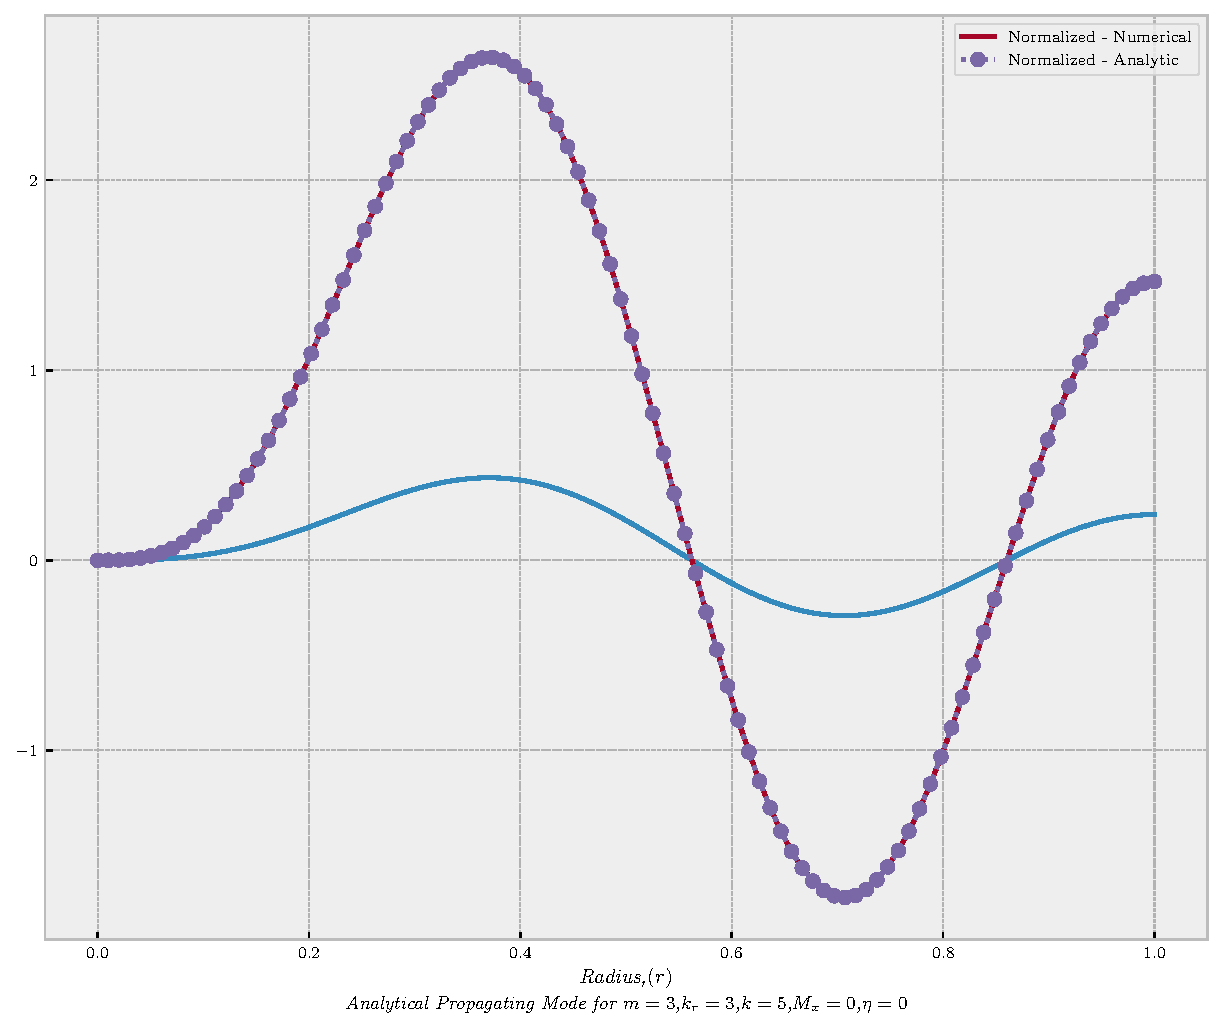
\includegraphics[width=0.5\textwidth]{Radial_mode_analytical_test_case.pdf}
    \end{figure}
\end{frame}
\begin{frame}
    \begin{figure}[!]
        \centering
        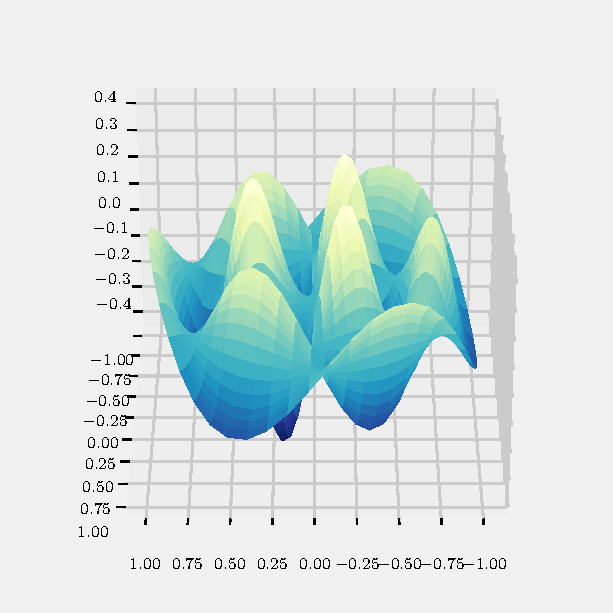
\includegraphics{Radial_mode_analytical_test_case_3d1.pdf}
    \end{figure}
\end{frame}
\begin{frame}
    \begin{figure}[!]
        \centering
        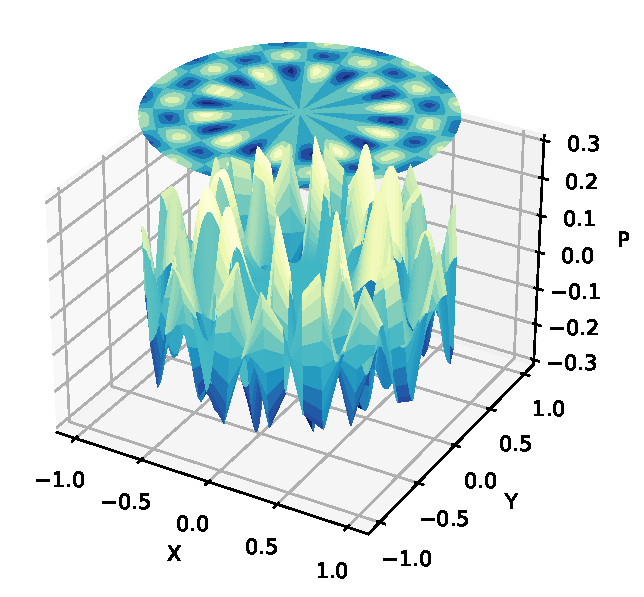
\includegraphics{Radial_mode_analytical_test_case_3d2.pdf}
    \end{figure}
\end{frame}

\begin{frame}
    \begin{figure}[!]
        \centering
        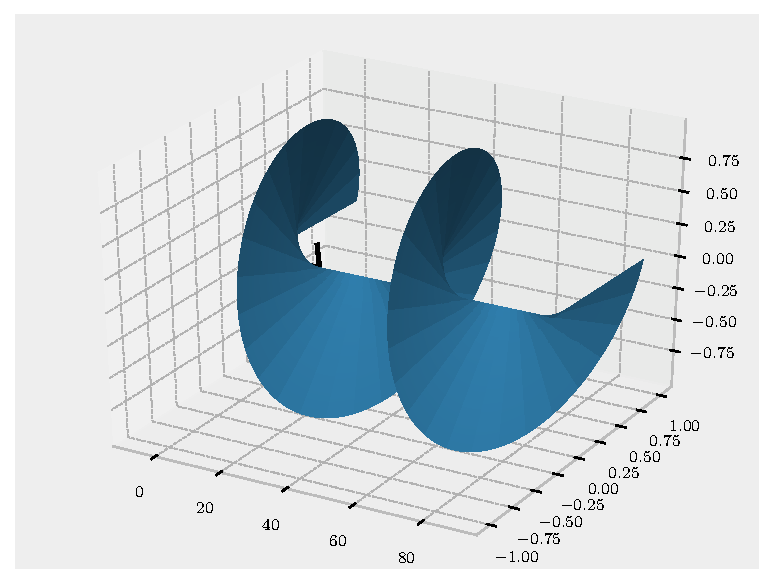
\includegraphics{helicoid_test_case_3d2.pdf}
    \end{figure}
\end{frame}
% \section{Results Update}
% \frame{\sectionpage}

% \begin{frame}{Motivation}
%     \begin{alertblock}{How is the analytical solution computed for Sound Prop. in Uniform Axial Flow}
%     \begin{enumerate}[<+->]\itemsep9pt
%         \item The analytical solution are the axial wavenumbers and propagating
%             modes for a given frequency, axial velocity and azimuthal mode order.
%         \item For a given azimuthal mode, there is a range of radial modes.
%         \item These radial modes can be categorized based on the sign of the axial wavenumber and if it is
%             complex in value. 
%         \item Propagating modes are defined by axial wavenumbers, $k_x$, that have a real-part only, yielding 
%             the assumed fluctuation to resemble Euler's Formula ($e^{ik_x x}$). 
%         \item On the other hand, if the $k_x$ is complex, then the mode will resemble an exponentially decaying
%             function since the imaginary number cancels, leaving a minus sign in front of
%             the axial wavenumber.
%     \end{enumerate}
%     \end{alertblock}

%     \tiny
%     % \hspace{3.75em}\url{http://www.klimaschutzplan2050.de/en/action-areas/energy-sector/}
% \end{frame}
% \begin{frame}

% \begin{equation}
%     k_x  = \frac{- M_x k \pm \sqrt{k^2 - ( 1 - M_x^2) J_{m,n}'^2 }}{\left( 1 - M_x^2 \right)}.
%     \label{eqn:ax_wavenumb}
% \end{equation}

% where $M_x$ is the axial Mach number, $k$ is the temporal (referred to as reduced)
% frequency, and $J_{m,n}'$ is the derivative of the Bessel function of the first kind.  
% The $\pm$ accounts for both upstream and downstream modes.

% The condition for propagation is such that the axial wavenumber is larger than 
% a ``cut-off'' value

% \begin{equation}
%     k_{x,real}  = \frac{\pm M_x k }{\left( M_x^2 - 1 \right)}.
%     \label{eqn:cuton}
% \end{equation}


% \end{frame}
% \begin{frame}
    
% Every term that is being raised to the one half i.e. square rooted must 
% be larger than zero to keep axial wavenumber from being imaginary. The mode 
% will propagate or decay based on this condition. Recall thaT the mode is of the 
% form 
% \begin{equation}
%     e^{i k_x x}
%     \label{eqn:fluctuationexample}
% \end{equation}
% if $k_x$ has a real part, $k_{x,real}$ and an imaginary part $i k_{x,imag}$ 
% then,

% \begin{align}
%     &= e^{i k_x x} \\
%     &= e^{i (k_{x,real}+ i k_{x,imag}) x} \\
%     &= \underbrace{e^{i k_{x,real}x}}_{\textit{amplitude}} \underbrace{e^{- k_{x,imag} x}}_{\textit{exponential decay}} 
% \end{align}


% \end{frame}
% \begin{frame}
    

% Although the ``cut-off'' decay to nearly zero rapidly, the rate at which this occured
% was not much of a concern earlier on in turbomachinery design. As nacelles 
% continue to grow shorter, a mode that is ``cut-off'' may make it outside the duct.

% For this work a desired amplitude was arbitrarily chosen for a mode, $y_{desired}$
% and then the axial location at which this occurred, $x_{desired}$ which 
% can be compared against a desired length for a nacelle.  
% Since SWIRL assumes an infinitely long duct, there is nothing limiting the 
% modes propagation with respect to nacelle length. For example, if the 
% desired amplitude is one percent, then $x_{desired}$,

% \begin{align*}
%     0.01 &=  e^{-10 x_{desired}},\\
%     -\frac{ln|0.01|}{10} &=  x_{desired},\\
%     -\frac{ln|0.01|}{10} &= 0.4605170185988091 .
% \end{align*}

% \end{frame}
% \begin{frame}
    


%  \begin{figure}
%      \centering
%      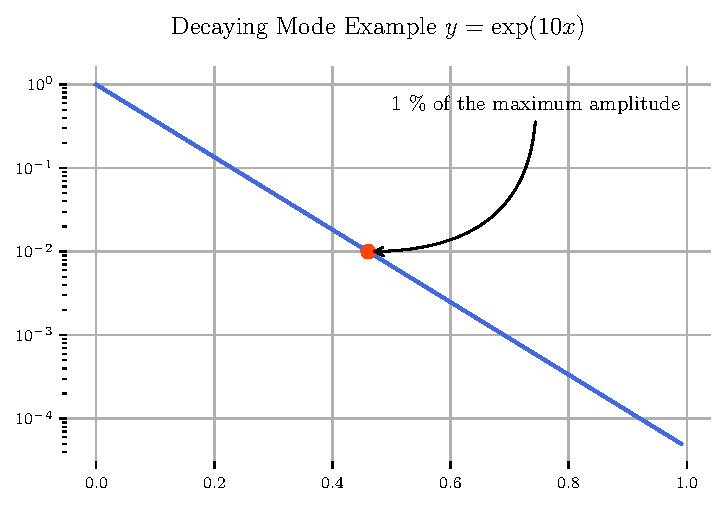
\includegraphics[width=0.7\textwidth]{/home/jeff-severino/SWIRL/CodeRun/04-plotReport/tex-outputs/desired_cut_off_location_1_percent_of_max2.pdf}
%      \caption{Decaying mode with $k_x = 0 + 10j$ and unit amplitude. One percent
%      of the maximum amplitude is identified for nacelle length comparison}
%      \label{fig:decaying_mode_with_1_percent_amp}
%  \end{figure}
 
 
% In general,
% \begin{align*}
%     y_{desired} &=  e^{-k_{x,imag} x_{desired} }\\
%     -\frac{ln|y_{desired}|}{k_{x,imag}} &=  x_{desired}
% \end{align*}
% \end{frame}
% \begin{frame}
% \section{Analytical Test Case 1}
% \begin{table}[h!]
%     \centering
%     \begin{tabular}{|l|l|}
%         \hline
%         $\sigma$ & \textit{0.0} \\ \hline
%         $k$      & \textit{10}   \\ \hline
%         $m$      & \textit{2}    \\ \hline
%         $M_x$    & \textit{0.3}  \\ \hline
%     \end{tabular}
%     \caption{Validation test case parameters, Uniform Flow Annular Duct} 
% \end{table}

% \end{frame}

% \begin{frame}
    
%  \begin{figure}
%      \centering
%      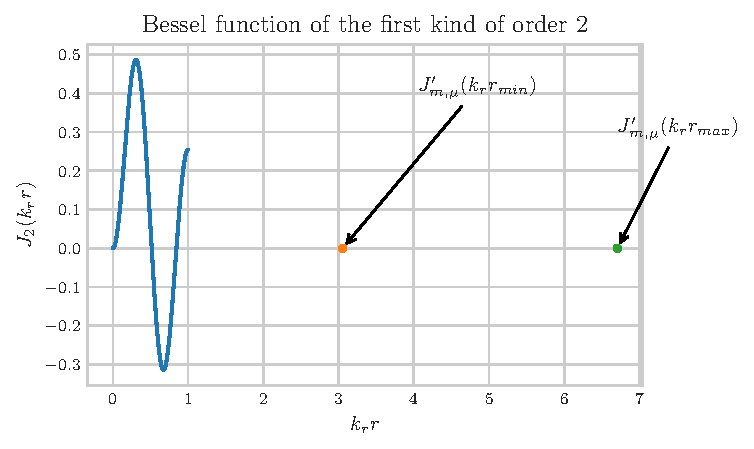
\includegraphics[width=0.7\textwidth]{/home/jeff-severino/SWIRL/CodeRun/04-plotReport/tex-outputs/bessel_analytical_test_case.pdf}
%      \caption{The Bessel function with the values of $J'_{m,\mu}$ labeled}
%      \label{fig:decaying_mode_with_1_percent_amp}
%  \end{figure}
% \end{frame}



% \begin{frame}
    
%  \begin{figure}
%      \centering
%      \includegraphics[width=0.7\textwidth]{/home/jeff-severino/SWIRL/CodeRun/04-plotReport/tex-outputs/axial_wavenumber_analytical_test_case.pdf}
%      \caption{The Bessel function with the values of $J'_{m,\mu}$ labeled}
%      \label{fig:decaying_mode_with_1_percent_amp}
%  \end{figure}
% \end{frame}


% \begin{frame}{Normalized Mode}

    
%  \begin{figure}
%      \centering
%      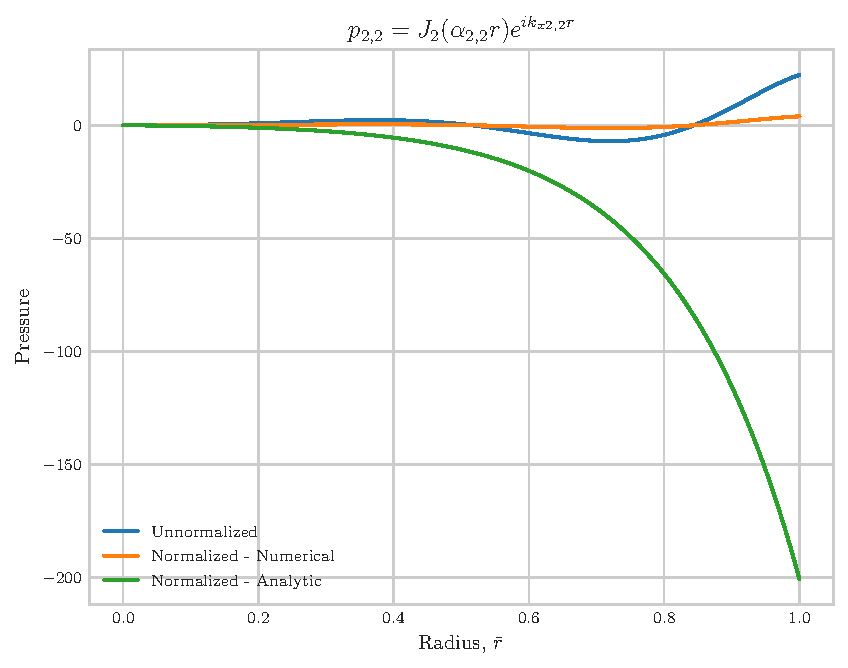
\includegraphics[width=0.7\textwidth]{/home/jeff-severino/SWIRL/CodeRun/04-plotReport/tex-outputs/Normalized_Mode_test_case.pdf}
%      \caption{The Bessel function with the values of $J'_{m,\mu}$ labeled}
%      \label{fig:decaying_mode_with_1_percent_amp}
%  \end{figure}
% \end{frame}
% \begin{frame}
    
% \end{frame}




% \begin{frame}{Future Work}
%     \begin{alertblock}{}
%     \begin{enumerate}[<+->]\itemsep9pt
%         \item I need to use sanity checks to ensure that the normalization provided
%             by Rienstra is implemented correctly.
%         \item While the numerical normalized mode has an integral of one, the 
%             analytical mode is not.
%         \item a few things that have been checked along the way but need to be 
%             reported are,
%         \item Zero's of $J'_m$ 
%         \item Value of $J_m$ at the zero location
%         \item Relations involving integrals If it so not too cumbersome.
%             There are some simplifications that could be checked\ldots 
%         \item Check the analytical test case that has been reported in literature.
%            The difference is that $\sigma = 0.25$
%     \end{enumerate}
%     \end{alertblock}

%     \tiny
%     % \hspace{3.75em}\url{http://www.klimaschutzplan2050.de/en/action-areas/energy-sector/}
% \end{frame}

% % \begin{frame}{Perspective}{Disciplines for investigating energy topics}
% %     \begin{center}
% %     \begin{tikzpicture}[
% %       node distance=4.5em and .75cm,font=\small
% %     ]
% %     % flowboxes
% %     \node[flowbox] (physik) {
% %         \fbtitle{Physics}\vphantom{yÖ}
% %     \nodepart{two}
% %         \begin{minipage}{.16\textwidth}
% %             \centering
% %             Theoretical\\ feasibility\\
% %             \scriptsize (Natural laws)
% %         \end{minipage}
% %     };

% %     \node[flowbox,right=of physik] (technik) {
% %         \fbtitle{Engineering}\vphantom{yÖ}
% %     \nodepart{two}
% %         \begin{minipage}{.16\textwidth}
% %             \centering
% %             Technical\\ feasibility\\
% %             \scriptsize (Technologies)
% %         \end{minipage}
% %     };

% %     \node[flowbox,right=of technik] (econ) {
% %         \fbtitle{Economy}\vphantom{yÖ}
% %     \nodepart{two}
% %         \begin{minipage}{.16\textwidth}
% %             \centering
% %             Economic\\ feasibility\\
% %             \scriptsize (Funding)
% %         \end{minipage}
% %     };

% %     \node[flowbox,right=of econ] (society) {
% %         \fbtitle{Society}\vphantom{yÖ}
% %     \nodepart{two}
% %         \begin{minipage}{.16\textwidth}
% %             \centering
% %             Social\\ feasibility\\
% %             \scriptsize (Decision space)
% %         \end{minipage}
% %     };

% %     \uncover<2->{%
% %         \draw [decorate,decoration={brace,amplitude=10pt,mirror},ultra thick,jdblue]
% %             ($(technik.south west) + (-.2em,-1em)$) --
% %             ($(econ.south east)    + (+.2em,-1em)$) coordinate[midway,yshift=-3.8em] (midpoint-below);
    
% %         \node[flowbox] at (midpoint-below) (tech-econ)  {
% %             \fbtitle{Techno-economic modelling}\vphantom{yÖ}
% %         \nodepart{two}
% %             \begin{minipage}{.4\textwidth}
% %                 \centering
% %                 How much energy?
% %                 For how much?\vphantom{yÖ}
% %             \end{minipage}
% %         };
% %     }
% %     \end{tikzpicture}
% %     \end{center}
% % \end{frame}


\subsection{Theory}

To relate the speed of sound to a given flow, the radial momentum equation
is used.  If the flow contains a swirling component,then the primitive variables 
are nonuniform through the flow, and mean flow assumptions are not valid. 
\begin{align*}
    \frac{\partial v_r}{\partial t} +
    v_r \frac{\partial v_r}{\partial r} + 
    \frac{v_{\theta}}{r} 
    \frac{\partial v_{\theta}}{\partial \theta} -
    \frac{v_{\theta}^2}{r} 
    v_x \frac{\partial v_r}{\partial x} =
    \frac{1}{\rho}\frac{\partial P}{\partial r}
\end{align*}

 To account to for this, the radial momentum is simplified by assuming the 
 flow is steady, the flow has no radial component. In addition, the viscous
 and body forces are neglected.  Then the radial pressure derivative term is
 set equal to the dynamic pressure term. Seperation of variables is applied.  

 \begin{align*}
     \frac{v_{\theta}^2}{r} = \frac{1}{\rho}\frac{\partial P}{\partial r} \\
 P = \int_{r}^{r_{max}} \frac{\rho V_{\theta}^2}{  r}
 \end{align*}

To show the work, we will start with the dimensional form of the equation and
differentiate both sides.  Applying separation of variables,
 \[
     \int_{r}^{r_{max}}
     \frac{\bar{\rho} v_{\theta}^2}{r} \partial r 
     =-\int_{P(r)}^{P(r_{max})}\partial p.
 \]

Since $\tilde{r} = r/r_{max}$,
\[r = \tilde{r}r_{max}.\]
Taking total derivatives (i.e. applying chain rule),
\[dr = d(\tilde{r}r_{max}) = d(\tilde{r})r_{max}, \]
Substituting these back in and evaluating the right hand side,
\[
    \int_{\tilde{r}}^{1} \frac{\bar{\rho} v_{\theta}^2}{\tilde{r}}\partial \tilde{r} 
    =P(1)-P(\tilde{r})
\]

For reference the minimum value of $\tilde{r}$ is,

\[\sigma = \frac{r_{max}}{r_{min}}\]

For the radial derivative, the definition of the speed of sound is utilized,
\[\frac{\partial A^2}{\partial r } =
\frac{\partial}{\partial r} \left( \frac{\gamma P}{\rho} \right).\]

Using the quotient rule, the definition of the speed of sound is extracted,

\begin{align*}
&= \frac{\partial P}{\partial r} \frac{\gamma \bar{\rho}}{\bar{\rho}^2} -
\left(
    \frac{\gamma P}{\bar{\rho}^2} 
\right) 
\frac{\partial \bar{\rho}}{\partial r}\\
&=  \frac{\partial P}{\partial r} \frac{\gamma }{\bar{\rho}} -
\left( \frac{A^2}{\bar{\rho}} \right) 
\frac{\partial \bar{\rho} }{\partial r}
\end{align*}

Using isentropic condition $ \partial P/A^2 = \partial \rho$, 

\begin{align*}
&= \frac{\partial P}{\partial r} \frac{\gamma }{\bar{\rho}} -
\left( \frac{1}{\bar{\rho}} \right) \frac{\partial  P }{\partial r}\\
\frac{\partial A^2}{\partial r} 
&= \frac{\partial P}{\partial r} \frac{\gamma - 1}{\bar{\rho}}  
\end{align*}

\begin{align*}
    \frac{\bar{\rho}}{\gamma -1}\frac{\partial A^2}{\partial r} &= \frac{\partial P}{\partial r} 
\end{align*}


Going back to the radial momentum equation, and rearranging the terms will simplify 
the expression. The following terms are defined to start the
nondimensionalization.  

\begin{align*}
    M_{\theta} &= \frac{V_{\theta}}{A} \\ 
    \widetilde{r} &= \frac{r}{r_{max}}  \\
    \widetilde{A} &= \frac{A}{A_{r,max}}  \\
    A &= \widetilde{A}{A_{r,max}} \\
    r &= \widetilde{r}{r_{max}}\\
    \frac{\partial}{\partial r} &=
    \frac{\partial \widetilde{r}}{\partial r} \frac{\partial}{\partial \widetilde{r}}\\
                                &= \frac{1}{r_{max}}\frac{\partial}{\partial \widetilde{r}}
\end{align*}
Dividing by $A$,
\begin{align*}
    \frac{M_{\theta}^2}{r}\left(\gamma - 1\right) 
 &= \frac{\partial A^2}{\partial r} \frac{1}{A^2}
\end{align*}

Now there is two options, either find the derivative of  $\bar{A}$ or the integral of
$M_{\theta}$ with respect to r.
\begin{enumerate}
    \item
%\begin{align*}
%\text{Integrating both sides } 
%\int_{r}^{r_{max}}\frac{M_{\theta}}{r}\left(\gamma - 1\right){\partial r}  &=\int_{A^2(r)}^{A^2(r_{max})}\frac{1}{A^2}  {\partial A^2}\\
%\int_{r}^{r_{max}}\frac{M^2_{\theta}}{r}\left(\gamma - 1\right){\partial r}  &=ln(A^2(r_{max})) - ln(A^2(r)) \\
%\int_{r}^{r_{max}}\frac{M^2_{\theta}}{r}\left(\gamma - 1\right){\partial r}  &=ln\left(\frac{A^2(r_{max})}{A^2(r)}\right) 
%\end{align*}
%
Defining non dimensional speed of sound $\tilde{A} = \frac{A(r)}{A(r_{max})}$
\begin{align*}
\int_{r}^{r_{max}}\frac{M_{\theta}}{r}\left(\gamma - 1\right){\partial r}  &=ln\left(\frac{1}{\tilde{A}^2}\right) \\
&= -2ln(\tilde{A})\\
\tilde{A}(r) &= exp\left[-\int_{r}^{r_{max}}\frac{M_{\theta}}{r}\frac{\left(\gamma - 1\right)}{2}{\partial r}\right] \\ \text{replacing r with }\tilde{r} \rightarrow \tilde{A}(r) &= exp\left[-\int_{r}^{r_{max}}\frac{M_{\theta}}{r}\frac{\left(\gamma - 1\right)}{2}{\partial r}\right]		\\
\tilde{A}(\tilde{r}) &= exp\left[\left(\frac{1 - \gamma}{2}\right)\int_{\tilde{r}}^{1}\frac{M_{\theta}}{\tilde{r}}{\partial \tilde{r}}\right]	
\end{align*}
\item Or we can differentiate
\end{enumerate}
Solving for $M_{\theta}$ ,
\begin{align*}
M_{\theta}^2 
&= \frac{\partial A^2}{\partial r} \frac{r}{A^2 \left(\gamma - 1\right)}
\end{align*}
Nondimensionalizing and substituting, 

\begin{align} 
    M_{\theta}^2
    \frac{\left( \gamma - 1 \right)}{\widetilde{r} r_{max}} &=
    \frac{1}{(\widetilde{A}A_{r,max})^2}\frac{A_{r,max}^2}{r_{max}}
    \frac{\partial \widetilde{A}^2}{\partial \widetilde{r}} \nonumber \\
    M_{\theta}^2     \frac{\left( \gamma - 1 \right)}{\widetilde{r} } &=
    \frac{1}{\widetilde{A}^2}
    \frac{\partial \widetilde{A}^2}{\partial \widetilde{r}} \nonumber \\
    M_{\theta} &= \sqrt{\frac{\widetilde{r}}{(\gamma-1) \widetilde{A}^2}
        \frac{\partial\widetilde{A}^2}{\partial \widetilde{r} }
    } \label{eq:Mthetabackcalculated}
\end{align}

% 3.1 Guidelines for Creating Manufactured Solutions states:
% \begin{enumerate}
%     \item  The manufactured solutions should be composed of smooth analytic 
%         functions 
%     \item The manufactured solutions should exercize every term in the governing
%         equation that is being tested,
%     \item The solution should have non trivial derivatives.  
%     \item The solution derivatives should be bounded by a small constant. In this case
%         this constant should prevent the function from becoming greater than 
%         one.
%     \item The solution should not prevent the code from running 
%     \item The solution should be defined on a connected subset of two- or three-
%         dimensional space to allow flexibility in chosing the domain of the PDE.
%         Section 3.3.1 provides more information about this.
%     \item The solution should coincide with the differential operators of the PDE.
%         For example, the flux term in Fourier's law of conduction requires T to 
%         be differentiable.
% \end{enumerate}
% With these guidelines, a function is specified for the speed of sound to conduct
% a method of manufactured solutions on SWIRL's speed of sound numerical 
% integration. This is checked by observing the tangential mach number 
% produced from the speed of sound and comparing that to the tangential mach number
% that has been analytically defined (See Equation \ref{eq:Mthetabackcalculated}).

%
\subsection{Procedure}
There are a few constraints and conditions that must be followed in order for the analytical 
function to work with SWIRL, 

\begin{itemize}
    \item The mean flow and speed of sound must be real and positive. This will 
        occur is a speed of sound is chosen such that the tangential mach number
        is imaginary
    \item The derivative of the speed of sound must be positive
    \item Any bounding constants used with the mean flow should not allow the 
        total Mach number to exceed one.
    \item the speed of sound should be one at the outer radius of the cylinder
\end{itemize}

Given these constraints, $tanh(r)$ is chosen as a function since it can be
modified to meet the conditions above. Literature (The tanh method: A tool for 
solving certain classes of nonlinear evolution and wave equations) 
is a paper than demonstrates the strength of using tanh functions.
One additonal benefit of tanh(r) is that it is bounded between one and negative one, i.e.

\begin{itemize}
    \item As r $\rightarrow$ $\infty$ tanh(r) $\rightarrow$ 1
    \item As -r $\rightarrow$ $-\infty$ tanh(r) $\rightarrow$ -1
\end{itemize}

To test the numerical integration method,  $M_{\theta}$ is defined as a result 
of differentiating the speed of sound, $A$. This is done opposed to integrating
$M_{\theta}$ analytically. However, an analytical function can be defined for
$M_{\theta}$, which can then be integrated to find what $\widetilde{A}$ should be. 
Instead, the procedure of choice is to back calculate what the appropriate 
$M_{\theta}$ is for a given expression for $\widetilde{A}$.  Since it is easier 
to take derivatives , we will solve for $M_{\theta}$ using Equation \ref{eq:Mthetabackcalculated} ,

\subsection{Tanh Summaion Formulation}
Knupp's Code Verification by the Method of Manufactured Solution (MMS) provides 
``guidelines'' for creating a manufactured solution (MS) such that the observed
order of accuracy will approach a theoretical order of accuracy as the number
of grid points are reduced from one iteration to the next. While these guidelines
offer a road map, there are choices that are left to the investigator that would
benefit from additional examples. The first guideline gives the user a free
choice of the MS as long as it s smooth. The benefit of the tanh summation method 
(TSM) reduces the difficuly in defining a sufficient MS by providing 
a general summation formulation that allows the user to Vary the number of 
terms in the MS, and the MS behavior without manually changing terms in the MS
symbolic expression. 

The general form of the MS will be a summation of $tanh$ bounded between zero
and one. A MS created with the TSM can provide a significant result for
a numerical differencing/integration technique by having inflection points of each
$tanh$ at various locations along the domain, giving a stair like slope.
While the TSM can add a layer of complexity to the MS that may not be needed, 
writing the formulation in a summation lends itself to iterative loops that can 
be coded, thus reducing the need for manual adjust of the MS, 
which can be an initial hurdle when performing MMS.


\section{General form of a Hyperbolic Tangent}

\begin{equation}
    R = A tanh(B(x-C)) 
    \label{eqn:1}
\end{equation}

\begin{equation}
    L = A tanh(B(C-E)) 
    \label{eqn:2}
\end{equation}
\begin{equation}
    y = R + L + D
    \label{eqn:3}
\end{equation}
where 
\begin{itemize}
    \item $R \equiv$ The value of the hyperbolic tangent. The variable $R$ represnts
        a ``right'' facing hyperbolic tangent kink.
    \item $A \equiv$ magnitude factor that increases or decreases the asymptotic
        limits $\lim_{x \to -\infty} = -1$ $\lim_{x \to \infty} = 1$
    \item $B \equiv$ ``steepness'' of the hyperbolic tangent
    \item $C \equiv$ The shift in inflection point of the hyperbolic tangent along the $
        x$ axis 
    \item $D \equiv$ The shift in inflection point of the hyperbolic tangent along the $
        y$ axis 
    \item $E \equiv$  $x_{i=i_{max}}$
    \item $x$ The domain. $x_i$ is used to indicate grid point indicies.
\end{itemize}
The idea is to sum up an arbitrary amount of tangents that will be bounded by zero
and one. 

\begin{figure}
    \centering
    \resizebox{\columnwidth}{!}{
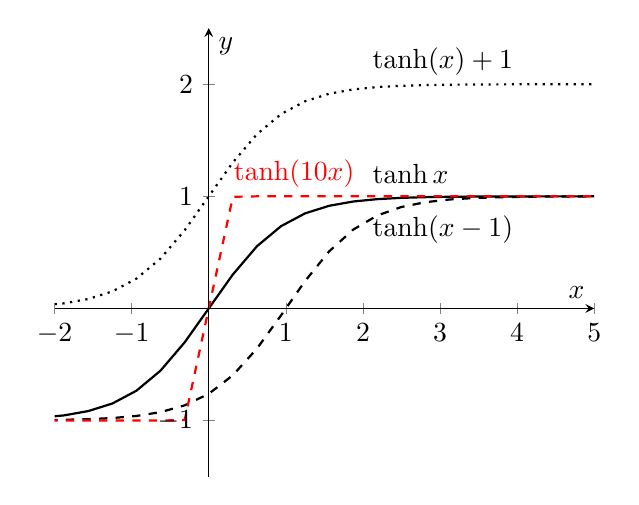
\begin{tikzpicture}
    \begin{axis}[
        xmin=-2, xmax=5,
        ymin=-1.5, ymax=2.5,
        axis lines=center,
        axis on top=true,
        domain=-2.5:5,
        ylabel=$y$,
        xlabel=$x$,
        ]

        \addplot [mark=none,draw= black, thick] {tanh(\x)};
        \node [right, black ] at (axis cs: 2,1.2) {$ \tanh x$};


        \addplot [mark=none,draw=black, dashed, thick] {tanh(\x - 1)};
        \node [right, black] at (axis cs: 2,0.7) {$ \tanh (x - 1)$};



        \addplot [mark=none,draw=red, dashed, thick] {tanh(10*\x)};
        \node [right, red] at (axis cs: 0.2,1.2) {$ \tanh (10x )$};



        \addplot [mark=none,draw=black, dotted, thick] {tanh(\x) + 1};
        \node [right, black] at (axis cs: 2,2.2) {$ \tanh (x) + 1$};

    \end{axis}
\end{tikzpicture}}
\end{figure}


Now the goal is to generalize this formulation such that we can add up terms.
$A$ is determined by setting a maximum amplitude for each $tanh$ function by
$A = A_{max}/n$. Note that amplitude can be different for each term but is chosen
to be the same. A parameter $\hat{x} = (x - x_{min})/ (x_{max} - x_{min}$ scales the domain to be between the  
minimum and maximum bounds.


\begin{equation}
    R_{ij} = A tanh(B(x_i-C_j)) 
    \label{eqn:1}
\end{equation}

\begin{equation}
    L_{j} = A tanh(B(C_j-E)) 
    \label{eqn:2}
\end{equation}
\begin{equation}
    y = \sum_{j = 1}^{n}  R_{ij} + \sum_{j = 1}^{n}L + D
    \label{eqn:3}
\end{equation}
The function \verb|TanhMethod| does this procedure. 

Setting $A = 1/16$ and $C_1  = 0$ , $C_2 = 0.75$ , $C_3 = 1$ , $D = 1$, $E = 1$  and 
$B = 10$


\begin{equation}
    \sum_{j = 1}^{3} R_{ij} = 1/16 tanh(10(\hat{x}_i))  + 1/16 tanh(10(\hat{x}_i-0.75)) + 1/16 tanh(10(\hat{x}_i-1))
    \label{eqn:1}
\end{equation}

\begin{equation}
    \sum_{j = 1}^{3} L_{j} = 1/16 tanh(10(-1))  + 1/16 tanh(10(0.75 - 1)) + 1/16 tanh(10(1-1))
    \label{eqn:1}
\end{equation}

The simplified expression becomes,
\begin{equation}
    y = \frac{1}{16}\tanh\left(\frac{100}{9}r - \frac{100}{9}\right) + \frac{1}{16}\tanh\left(\frac{100}{9}r -\frac{55}{9}\right) + \frac{1}{16}\tanh\left(\frac{100}{9}r -\frac{10}{9} \right) + \frac{7}{8}
\end{equation}


%\begin{figure}
%    \centering
%    \resizebox{\columnwidth}{!}{
%% This file was created with tikzplotlib v0.10.1.
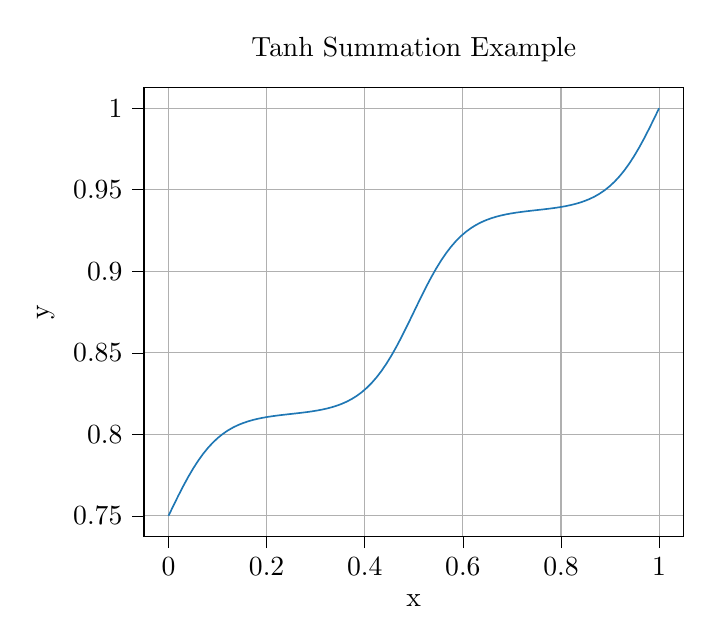
\begin{tikzpicture}

\definecolor{darkgray176}{RGB}{176,176,176}
\definecolor{steelblue31119180}{RGB}{31,119,180}

\begin{axis}[
tick align=outside,
tick pos=left,
title={Tanh Summation Example},
x grid style={darkgray176},
xlabel={x},
xmajorgrids,
xmin=-0.05, xmax=1.05,
xtick style={color=black},
y grid style={darkgray176},
ylabel={y},
ymajorgrids,
ymin=0.737511917481587, ymax=1.01249943250088,
ytick style={color=black}
]
\addplot [semithick, steelblue31119180]
table {%
0 0.750011349982464
0.0101010101010101 0.756304367923548
0.0202020202020202 0.762471427961815
0.0303030303030303 0.768396284241735
0.0404040404040404 0.773980954849054
0.0505050505050505 0.779151246168556
0.0606060606060606 0.78385900159005
0.0707070707070707 0.788081304133098
0.0808080808080808 0.791817372304981
0.0909090909090909 0.795084105493723
0.101010101010101 0.797911187966577
0.111111111111111 0.80033644822293
0.121212121212121 0.802401902498815
0.131313131313131 0.804150668035091
0.141414141414141 0.805624753143957
0.151515151515152 0.806863623924088
0.161616161616162 0.807903399550648
0.171717171717172 0.808776520778204
0.181818181818182 0.809511752175423
0.191919191919192 0.810134404577104
0.202020202020202 0.810666691986701
0.212121212121212 0.811128162249061
0.222222222222222 0.811536161419119
0.232323232323232 0.81190630759737
0.242424242424242 0.812252961565677
0.252525252525253 0.812589689584715
0.262626262626263 0.812929718947268
0.272727272727273 0.813286389915873
0.282828282828283 0.813673608902656
0.292929292929293 0.814106307344292
0.303030303030303 0.814600908628971
0.313131313131313 0.815175801361504
0.323232323232323 0.815851810708233
0.333333333333333 0.816652649865894
0.343434343434343 0.817605320080265
0.353535353535354 0.81874040944222
0.363636363636364 0.820092217733837
0.373737373737374 0.82169860781786
0.383838383838384 0.82360045643945
0.393939393939394 0.825840555061835
0.404040404040404 0.828461805118854
0.414141414141414 0.831504577298413
0.424242424242424 0.835003179865009
0.434343434343434 0.838981523240156
0.444444444444444 0.84344828154901
0.454545454545455 0.848392114910775
0.464646464646465 0.853777768834061
0.474747474747475 0.859544011154561
0.484848484848485 0.865604291561671
0.494949494949495 0.871850642171087
0.505050505050505 0.878160707811378
0.515151515151515 0.884407058420794
0.525252525252525 0.890467338827903
0.535353535353535 0.896233581148403
0.545454545454546 0.901619235071689
0.555555555555556 0.906563068433454
0.565656565656566 0.911029826742308
0.575757575757576 0.915008170117455
0.585858585858586 0.918506772684051
0.595959595959596 0.92154954486361
0.606060606060606 0.924170794920629
0.616161616161616 0.926410893543014
0.626262626262626 0.928312742164604
0.636363636363636 0.929919132248627
0.646464646464647 0.931270940540244
0.656565656565657 0.9324060299022
0.666666666666667 0.93335870011657
0.676767676767677 0.934159539274231
0.686868686868687 0.93483554862096
0.696969696969697 0.935410441353493
0.707070707070707 0.935905042638172
0.717171717171717 0.936337741079808
0.727272727272727 0.936724960066591
0.737373737373737 0.937081631035197
0.747474747474748 0.937421660397749
0.757575757575758 0.937758388416787
0.767676767676768 0.938105042385094
0.777777777777778 0.938475188563345
0.787878787878788 0.938883187733403
0.797979797979798 0.939344657995763
0.808080808080808 0.939876945405361
0.818181818181818 0.940499597807041
0.828282828282828 0.94123482920426
0.838383838383838 0.942107950431816
0.848484848484849 0.943147726058376
0.858585858585859 0.944386596838507
0.868686868686869 0.945860681947373
0.878787878787879 0.947609447483649
0.888888888888889 0.949674901759534
0.898989898989899 0.952100162015887
0.909090909090909 0.954927244488741
0.919191919191919 0.958193977677483
0.929292929292929 0.961930045849366
0.939393939393939 0.966152348392414
0.94949494949495 0.970860103813909
0.95959595959596 0.97603039513341
0.96969696969697 0.981615065740729
0.97979797979798 0.98753992202065
0.98989898989899 0.993706982058916
1 1
};
\end{axis}

\end{tikzpicture}

%}
%\end{figure}
%The goal is generate an MS with a number of ``stairs'' that is bounded between
%zero and one. Here's what my focus group ideas are,
%
%\begin{align*}
%    1 = R + L 
%\end{align*}
%where, 1 is a constraint, and R and L are the two waves when summed need to cancel 
%if it were the exact same amplitude \& opposite sign 
%
%so ,
%
%\begin{align*}
%    R + L = \tanh(x) + -\tanh(x) = 0
%\end{align*}
%or in our case,
%
%\begin{align*}
%    R + L = \tanh(x) + -\tanh(x) = 1
%\end{align*}
%
%We can tweak this by adding knobs by adding ``knobs'' A and B. If we dont want 
%the total to not exceed one then, $A_j + A_{j+1} \cdots A_{last} = 1$. $B_1$ changes
%the steepnes of the kink that we want. In order to generalize this,
%
%
%\begin{align*}
%    \bar{A} = \sum_{j=1}^n R_{ij} + \sum_{j=1}^n L_{ij} 
%\end{align*}
%where,
%\begin{align*}
%    R_{ij} = A_j \tanh(B_j (x_i - x_j)) \\ 
%    L_{ij} = A_j \tanh(B_j (x_j - x_n))  
%\end{align*}
%
%Letting $n = 3 \ldots$
%
%\begin{align*}
%    \bar{A} &= S_{vert} + \sum_{j=1}^3 R_{ij} + \sum_{j=1}^3 L_{ij} \\
%    \bar{A} &=
%    A_1 \tanh(B_1 (x_i - x_1))  + 
%    A_{2} \tanh(B_{2} (x_i - x_{2}))  + 
%    A_{3} \tanh(B_{3} (x_i - x_3)) +  \\
%    A_1 \tanh(B_1 (x_1 - x_n)) &+ 
%    A_{2} \tanh(B_{2} (x_2 - x_{n}))  +
%    A_{3} \tanh(B_{3} (x_3 - x_n))  
%\end{align*}
%and,
%\begin{align*}
%    A_1 = A_2 = A_3 = k_1 \\ 
%    B_1 = B_2 = B_3 = k_2  
%\end{align*}
%
A tanh summation method was constructed to make a manufactured solution with 
strong changes in slope. This ensures that the numerical approximation will not 
give trivial answers. 
then for some functions we need to impose boundary conditions. We will demonstrate
how the careless implementation of a boundary condition can lead to close approximations
on the interior.  The speed of sound is defined with the subscript $analytic$ to indicate that this is the analytical function of choice and has no physical relevance 
to the actual problem.

\begin{align*}
\widetilde{A}_{analytic} = \Lambda + k_1 \tanh \left( k_2 \left( \widetilde{r} - \widetilde{r}_{max} \right) \right),
\end{align*}

where, 

\begin{align*}
    \Lambda = 1 - k_1 \tanh(k_2 (1 - \widetilde{r}_{max})),
\end{align*}

When, $\widetilde{r}=\widetilde{r}_{max}$ , $\widetilde{A}_{analytic} = 1$.  
Taking the derivative with respect to $\widetilde{r}$,

\begin{align*}
    \frac{\partial \widetilde{A}_{analytic} }{\partial \widetilde{r}} &=
    \left(1 - \tanh^{2}{\left(\left(r - r_{max}\right) {k}_{2} \right)}\right) {k}_{1} {k}_{2}, \\ 
    &= \frac{ k_{1} k_{2}}{\cosh^{2}{\left(\left(r - r_{max}\right) {k}_{2} \right)}}.
\end{align*}

Substitute this into the expression for $M_{\theta}$ in Equation 
\ref{eq:Mthetabackcalculated},

\begin{align*}
    M_{\theta} = \sqrt{2}
    \sqrt{\frac{r {k}_{1} {k}_{2}}{\left(\kappa - 1\right) \left(\tanh{\left(\left(r - r_{max}\right) {k}_{2} \right)} {k}_{1} + \tanh{\left(\left(r_{max} - 1\right) {k}_{2} \right)} {k}_{1} + 1\right) \cosh^{2}{\left(\left(r - r_{max}\right) {k}_{2} \right)}}}
\end{align*} 

Now that the mean flow is defined, the integration method used to obtain the 
speed of sound

% What happens when $r = r_{max}$?

Initially the source terms were defined without mention of the indices of the 
matrices they make up. In other words, there was no fore sight on the fact that
these source terms are sums of the elements within A,B, and X. To investigate 
the source terms in greater detail, the FORTRAN code that calls the source 
terms will output the terms within the source term and then sum them, instead 


of just their sum.
i
$ [A]{x} = \lambda [B] {x} $

which can be rearranged as,

$ [A]{x} - \lambda [B] {x} = 0$

Here, $x$ is an eigenvector composed of the perturbation variables, $v_r,v_{\theta},v_x,p$ and $\lambda$ is the associated eigenvalue, (Note: $\lambda = -i \bar{\gamma}$)

Writing this out we obtain $\cdots$.

Linear System of Equations:
\begin{equation}
    -
    i \left(
        \frac{k}{A} - \frac{m}{r} M_{\theta}
    \right)
    v_r 
    -
    \frac{2}{r} M_{\theta} v_{\theta} 
    +
    \frac{dp}{dr} 
    +
    \frac{(\kappa - 1)}{r} M_{\theta}^2 p
    -
    \lambda M_x v_r =S_1
\end{equation}

Using matrix notation,

\begin{equation}
    A_{11}
    x_1 
    -
    A_{12} x_2 
    +
    A_{14} x_4
    -
    \lambda B_{11} x_1 = S_1
\end{equation}


But $A_{14}$ and $A_{41}$ in Kousen's paper only has the derivative operator.
Since I am currntly writing the matrix out term by term and not doing the matrix 
math to obtain the symbolic expressions, I will define $A_{14}$ with $dp/dr$ 
and $A_{41}$ with $dv_r/dr$
Similarly,
\begin{align}
    A_{21} x_1 &-
    A_{22} x_2 +
    A_{24} x_4 &-
    \lambda B_{22} x_2 &= S_2 \\
    A_{31} x_1 &-
    A_{33} x_3 &-
    \lambda (B_{33} x_3 + B_{34} x_4) &= S_3\\
    A_{41} x_1 &+
    A_{42} x_2 +
    A_{44} x_4 &- 
    \lambda (B_{33} x_3 + B_{44} x_4) &= S_4
\end{align}
Now we can begin looking at the source terms, term by term. They each should also
converge at a known rate







\subsection{Calculation of Observed Order-of-Accuracy}
The numerical scheme used to perform the integration of the tangential velocity
will have a theoretical order-of-accuracy. To find the theoretical 
order-of-accuracy, the discretization error must first be defined. The error, 
$\epsilon$, is a function of id spacing, $\Delta r$

\[ \epsilon = \epsilon(\Delta r) \]

The discretization error in the solution should be proportional to 
$\left( \Delta r \right)^{\alpha}$ where $\alpha > 0$ is the theoretical order
for the computational method.  The error for each grid is expressed as 
\[ \epsilon_{M_{\theta}}(\Delta r) = |M_{\theta,analytic}-M_{\theta,calc}|\]
where $M_{\theta,analytic}$ is the tangential mach number that is defined from the
speed of sound we also defined and the $M_{\theta,calc}$ is the result from 
SWIRL. The $\Delta r$ is to indicate that this is a discretization error for a
specific grid spacing. Applying the same concept to to the speed of sound,

If we define this error on various grid sizes and compute $\epsilon$ for
each grid, the observed order of accuracy can be estimated and compared to
the theoretical order of accuracy. For instance, if the numerical soution
is second-order accurate and the error is converging to a value, the L2 norm of
the error will decrease by a factor of 4 for every halving of the grid cell 
size. 

Since the input variables should remain unchanged (except from minor changes 
from the Akima interpolation), the error for the axial and tangential mach 
number should be zero. As for the speed of sound, since we are using an analytic
expression for the tangential mach number, we know what the theoretical result
would be from the numerical integration technique as shown above. 
Similarly we define the discretization error for the speed of sound.

\[ \epsilon_{A}(\Delta r) = |A_{analytic}-A_{calc}|\]

For a perfect answer, we expect $\epsilon$ to be zero. Since a Taylor series can 
be used to derive the numerical schemes, we know that the truncation of higher
order terms is what indicates the error we expect from using a scheme that 
is constructed with such truncated Taylor series.

The error at each grid point $j$ is expected to satisfy the following,

\begin{align*}
    0 &= |A_{analytic}(r_j) - A_{calc}(r_j)| \\
    \widetilde{A}_{analytic}(r_j) &= \widetilde{A}_{calc}(r_j) +
    (\Delta r)^{\alpha} \beta(r_j)  + H.O.T
\end{align*}

where the value of $\beta(r_j)$ does not change with grid spacing, and 
$\alpha$ is the asymptotic order of accuracy of the method. It is important to
note that the numerical method recovers the original equations as the grid 
spacing approached zero.  It is important to note that $\beta$ represents the
first derivative of the Taylor Series.  Subtracting $A_{analytic}$ from both
sides gives,

\begin{align*}
    A_{calc}(r_j) - A_{analytic}(r_j) &= A_{analytic}(r_j) - A_{analytic}(r_j)
    + \beta(r_j) (\Delta r)^{\alpha} \\
    \epsilon_A(r_j)(\Delta r) &= \beta(r_j) (\Delta r)^{\alpha}
\end{align*}

To estimate the order of accuracy of the accuracy, we define the global errors 
by calculating the L2 Norm of the error which is denoted as $\hat{\epsilon}_A$ 

\begin{align*}
    \hat{\epsilon}_A = \sqrt{\frac{1}{N}\sum_{j=1}^{N} \epsilon(r_j)^2  }
\end{align*}

\begin{align*}
    \hat{\beta}_A(r_j) = \sqrt{\frac{1}{N}\sum_{j=1}^{N} \beta(r_j)^2  }
\end{align*}

As the grid density increases, $\hat{\beta}$ should asymptote to a constant 
value. Given two grid densities, $\Delta r$ and $\sigma\Delta r$, and assuming
that the leading error term is much larger than any other error term,

\begin{align*}
    \hat{\epsilon}_{grid 1} &= \hat{\epsilon}(\Delta r) = \hat{\beta}(\Delta r)^{\alpha} \\
    \hat{\epsilon}_{grid 2} &= \hat{\epsilon}(\sigma \Delta r) = \hat{\beta}(\sigma \Delta r)^{\alpha} \\
                            &= \hat{\beta}(\Delta r)^{\alpha} \sigma^{\alpha}
\end{align*}

The ratio of two errors is given by,

\begin{align*}
    \frac{\hat{\epsilon}_{grid 2}}{\hat{\epsilon}_{grid 1}} &= 
    \frac{\hat{\beta}(\Delta r )^{\alpha}}{\hat{\beta}(\Delta r )^{\alpha}} \sigma^{\alpha} \\ &= \sigma^{\alpha}
\end{align*}

Thus, $\alpha$,the asymptotic rate of convergence is computed as follows 

\begin{align*}
    \alpha = \frac{
        \ln \frac{
            \hat{\epsilon}_{grid 2}
    }{\hat{\epsilon}_{grid 1} }}
    {\ln\left( \sigma \right) }
\end{align*}

Defining  for a doubling of grid points ,
%
%\begin{align*}
%    \alpha = \frac{\ln \left( \hat{\epsilon}\left( \frac{1}{2}\Delta  r\right)
%            \right) -\ln \left( \hat{\epsilon}\left( \Delta  r\right)
%    \right)}{\ln \left( \frac{1}{2} \right)}
%\end{align*}
%
Similarly for the eigenvalue problem, 

\[ [A]x = \lambda [B]x \]




[~Insert your text to chapter 2 here. A pretend example of a silly
figure is provided below (i.e., Figure~\ref{DOWD}).~]

%        +----------------------------------------------------------+
%        |                                                          |
%        |  IMPORTANT:                                              |
%        |                                                          |
%        |  Delete the following material.  I included this         |
%        |  material here as a silly figure to provide an example   |
%        |  in the List of Figures page for this template file.     |
%        |                                                          |
%        +----------------------------------------------------------+

      \vfill
      % \begin{figure}[ht]
      % \begin{center}
      % \begin{tabular}{|cp{5.5in}c|} \hline
      % & Let's pretend that instead of this text I provided a figure
      % of myself smoking a most excellent cigar.  As long as we're
      % pretending, let's assume that figure shows that I have a really
      % big smile on my face. & \\
      % & & \\[-0.75em]
      % & OK, the truth is that I wanted to provide an example of a
      % figure to contrast the text in the figure's caption to the text
      % entered as a entry in the \emph{List of Figures}. This
      % difference is controlled through the
      % $\backslash$\texttt{caption[\,]\{\}} command. Appendix~B of
      % ``Read Me First (v12).pdf'' provides a primer for this issue. &
      % \\ \hline
      % \end{tabular}
      % \caption[Dr.~Dowd enjoying a wonderful cigar.] {Dr.~Dowd
      %         enjoying a wonderful cigar. From the smile on his face
      %         we are left to wonder if the cigar is an H.~Upmann
      %         \emph{Corona Imperial} or a Punch \emph{Rothchild}
      %         (with a double maduro wrapper, of course). \label{DOWD}
      %         }
      % \end{center}
      % \end{figure}
      \vfill

%XXXXXXXXXXXXXXXXXXXXXXXXXXXXXXXXXXXXXXXXXXXXXXXXXXXXXXXXXXXXXXXXXXXX
%XXXXXXXXXXXXXXXXXXXXXXXXXXXXXXXXXXXXXXXXXXXXXXXXXXXXXXXXXXXXXXXXXXXX
%XXXXXXXXXXXXXXXXXXXXXXXXXXXXXXXXXXXXXXXXXXXXXXXXXXXXXXXXXXXXXXXXXXXX
%XXXXXXXXXXXXXXXXXXXXXXXXXXXXXXXXXXXXXXXXXXXXXXXXXXXXXXXXXXXXXXXXXXXX

%--------+----------------------------------------------------------+
%        |  \myreferences{}                          (CONDITIONAL)  |
%        |                                                          |
%        |  See section 3.18 of "Read_Me_First_(v12).pdf"           |
%        |                                                          |
%        |  That section of the READ ME file describes two options  |
%        |  for listing the works cited in your document: first,    |
%        |  manually entering your list of references and, second,  |
%        |  using BibTeX to generate that list.                     |
%        |                                                          |
%        |  1) If you manually enter your reference list, first     |
%        |     include the \myreferences command, as illustrated    |
%        |     below.  Second, use the "referencelist" environment  |
%        |     described below.  For this, note that the UT Manual  |
%        |     requires double-spacing *between* references in      |
%        |     that list. However, it also states that *within*     |
%        |     individual references the spacing may be single- or  |
%        |     double-spaced.  Because of this, UThesis provides    |
%        |     two options for the "referencelist" environment:     |
%        |                                                          |
%        |            \begin{referencelist}{ENTER OPTION HERE}      |
%        |            \item ...                                     |
%        |            \end{referencelist}                           |
%        |                                                          |
%        |     a. Replacing "ENTER OPTION HERE" above with the      |
%        |        text "single" will generate a reference list      |
%        |        with single-spaced entries in that list but       |
%        |        double-spacing between those entries. An example  |
%        |        of this is provided below.                        |
%        |     b. Alternatively, using the "double" option will     |
%        |        generate a list with double-spaced entries and    |
%        |        double-spacing between entries. An example of     |
%        |        this is also provided below.                      |
%        |                                                          |
%        |     Note that input to these options is case sensitive   |
%        |     and the default setting is the "double" option.      |
%        |                                                          |
%        |  2) If you instead choose to use BibTeX to generate the  |
%        |     reference list, then you *cannot* include either     |
%        |     the "\myreferences" command or the "referencelist"   |
%        |     environment in your document. In this case you must  |
%        |                                                          |
%        |     a. delete the \myreferences command and the two      |
%        |        examples of the "referencelist"  environment      |
%        |        below;                                            |
%        |     b. then you must add and locate appropriately all    |
%        |        necessary BibTeX commands within your document    |
%        |        (e.g., \bibliographystyle{}, \citationstyle{},    |
%        |        \bibliography{}, etc.).                           |
%        +----------------------------------------------------------+
%
%\myreferences
%
%                                          %%%%%%%%%%%%%%%%%%%%%%
%                                          %% DELETE THIS WHEN
% \hfill \fbox{First example: references   %% CONSTRUCTING YOUR
% generated by the ``single'' option}      %% OWN REFERENCE LIST
%                                          %%%%%%%%%%%%%%%%%%%%%%
%
%\begin{referencelist}{single}
%\item \textbf{Friedman, Milton}, ``The Role of Monetary Policy,''
%      \emph{American Economic Review}, March 1968, 58(1), 1--17.
%
%\item \textbf{Keynes, John Maynard}, \emph{The General Theory of
%      Employment, Interest, and Money}, New York: Harcourt Brace
%      Jovanovic, 1936.
%
%\item \textbf{Smith, Adam}, \emph{An Inquiry into the Nature and
%      Causes of the Wealth of Nations}, Edwin Cannan, ed.,
%      London: Methuen \& Co., Ltd. 1904.
%
%\item \textbf{Tobin, James}, ``A Dynamic Aggregative Model,''
%      \emph{Journal of Political Economy,} April 1955, 63(2),
%      103--115.
%\end{referencelist}
%
%                                          %%%%%%%%%%%%%%%%%%%%%%
%                                          %% DELETE THIS WHEN
% \hfill \fbox{Second example: references  %% CONSTRUCTING YOUR
% generated by the ``double'' option}      %% OWN REFERENCE LIST
%                                          %%%%%%%%%%%%%%%%%%%%%%
%
%\begin{referencelist}{double}
%\item \textbf{Friedman, Milton}, ``The Role of Monetary Policy,''
%      \emph{American Economic Review}, March 1968, 58(1), 1--17.
%
%\item \textbf{Keynes, John Maynard}, \emph{The General Theory of
%      Employment, Interest, and Money}, New York: Harcourt Brace
%      Jovanovic, 1936.
%
%\item \textbf{Smith, Adam}, \emph{An Inquiry into the Nature and
%      Causes of the Wealth of Nations}, Edwin Cannan, ed.,
%      London: Methuen \& Co., Ltd. 1904.
%
%\item \textbf{Tobin, James}, ``A Dynamic Aggregative Model,''
%      \emph{Journal of Political Economy,} April 1955, 63(2),
%      103--115.
%\end{referencelist}

%XXXXXXXXXXXXXXXXXXXXXXXXXXXXXXXXXXXXXXXXXXXXXXXXXXXXXXXXXXXXXXXXXXXX
%XXXXXXXXXXXXXXXXXXXXXXXXXXXXXXXXXXXXXXXXXXXXXXXXXXXXXXXXXXXXXXXXXXXX
%XXXXXXXXXXXXXXXXXXXXXXXXXXXXXXXXXXXXXXXXXXXXXXXXXXXXXXXXXXXXXXXXXXXX
%XXXXXXXXXXXXXXXXXXXXXXXXXXXXXXXXXXXXXXXXXXXXXXXXXXXXXXXXXXXXXXXXXXXX

%--------+----------------------------------------------------------+
%        |  \appendix                                  (IF NEEDED)  |
%        |                                                          |
%        |  See section 3.19 of "Read_Me_First_(v12).pdf"           |
%        |                                                          |
%        |  1) When you include the \appendix command a subsequent  |
%        |     \chapter{} command will not generate a chapter but   |
%        |     an appendix section.                                 |
%        |                                                          |
%        |  2) As is illustrated below, to generate a second or     |
%        |     third appendix you simply have to include            |
%        |     additional \chapter{} commands (i.e., you DO NOT     |
%        |     have to repeat the use of the \appendix command).    |
%        +----------------------------------------------------------+
\bibliography{references}
      \bibliographystyle{unsrt}
\appendix

\chapter{Chapter 3 Appendix}
\section{Appendix A: Speed of Sound}

Sound wave is a pressure disturbance that moves with at a speed $a$
%%
%\begin{figure}[h!]
%	\centering
%	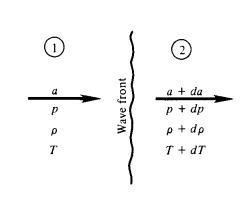
\includegraphics[width=0.3\linewidth]{screenshot001.png}
%	\label{fig:screenshot001}
%\end{figure}
%
By applying a rectangular control volume around this pressure wave, we can apply our conservation equations. We are assuming that these properities are increasing by a small increment. This is why each variable is added by a infinitesimally small term.

Recalling the conservation of mass (continuity equation), $\dot{m} = constant$

\[\dot{m}_{left} = \dot{m}_{right}\]

Recalling he definition of density, $\rho = m/\bar{V}$ and rewriting $\bar{V} = uA$ (check the units)
\[\rho a \cancel{A}  = (\rho + d\rho)(a + da) \cancel{A}\]
Futher expanding gives,
\[\rho a   = (\rho a+ \rho da + a d\rho + da d\rho)\]

We say that $da d\rho$ is so small, we can assume it is zero. This is often referred to as "neglecting higher order terms (H.O.T)". The expression then becomes

\[\frac{da}{a} = -\frac{d \rho}{\rho}\]

For the momentum equation $P + \rho u^2 = constant$
\[P + \rho a^2  = P + dP +  (\rho + d\rho)(a + da)(a + da) \]

But we just said that $\rho a = (\rho + d\rho)(a + da)$


\[P + \rho a^2  = P + dP +  \rho a(a + da) \]
\[dP + \rho ada = a\]

Multiplying the second term by a and divide by a, this is essentially multiplying the second term by one.

\[dP + \rho a^2\frac{da}{a} = a\]

recalling the relation $\frac{da}{a} = -\frac{d \rho}{\rho}$

\[dp - a^2 d \rho = 0\]

                       \[a^2 = \frac{dp}{d\rho}\]

Since a sound wave is a very weak wave, when it travels through a medium, it only increases the pressure and density, etc. slightly. The effect of this is that friction  and heat transfer can be neglected. Since friction cannot be undone, we call this an irreversible process. Whenever there is no transfer of heat, it is called this adiabatic. Thus, the propagation of sound is an adiabatic, reversible process, otherwise called isentropic. Isentropic implies no increase in entropy, which is \textit{not} true in the presence of shock waves.

In the case of a thermally perfect gas, we can say $P = \rho R T$

For a callorically perfect gas we can say $pv^{\gamma} = constant$, where $v$ is volume per unit mass, or specific volume

Differentiating and recalling that $v = 1/\rho$

\[a = \sqrt{\frac{\gamma P}{\rho}} = \sqrt{\gamma R T}\]


\[dm = \left( \rho u\right)_2 - \left(\rho u\right)_1\]
\[D(mV) = \left(\rho u^2 + P \right)_2\]

For Steady flow,

\[\cancel{dm} = \left( \rho u\right)_2 - \left(\rho u\right)_1\]

\[ \left( \rho u\right)_1 = \left(\rho u\right)_2\]

Similarly, for the Momentum equation,

\[\left(\rho u^2 + P\right)_1 = \left(\rho u^2 + P\right)_2\]

Let us change the coordinate system motion for the traveling wave be independent of time, and thus corresponds to \textit{steady state} wave propagation. 
\[ u_1 = \bar{u} + a - \frac{1}{2} \partial u \]
\[ u_2 = \bar{u} + a + \frac{1}{2} \partial u \]


where, $\bar{u}$ is the average flow velocity and $a$ is the wave speed.


Substituting this back into the conservation of mass

\[\left(\rho u\right)_1 = \left(\rho u\right)_2 \]

\[ 
\left( \rho    - \frac{1}{2}\partial \rho \right) 
\left( \bar{u} - a - \frac{1}{2}\partial u\right) = 
\left( \rho    + \frac{1}{2}\partial \rho \right) 
\left( \bar{u} - a + \frac{1}{2}\partial u\right) 
\]

Further expanding

\[
\cancel{
	\rho \bar{u} - \rho a
} + 
\frac{1}{2} 
\left(
-\rho \partial u - \bar{u} - \bar{u} \partial \rho + a \partial \rho 
\right) +
\cancel{
	\frac{1}{4}\partial \rho \partial u 
}
= 
\cancel{
	\rho \bar{u} - \rho a
} + 
\frac{1}{2} 
\left(
\rho \partial u + \bar{u} - \bar{u} \partial \rho - a \partial \rho 
\right) +
\cancel{
	\frac{1}{4}\partial \rho \partial u 
}
\]
 
\[
  \frac{1}{2}\left( - \rho \partial u - \bar{u} \partial \rho + a \partial \rho\right) = 
  \frac{1}{2}\left(   \rho \partial u + \bar{u} \partial \rho - a \partial \rho\right)
\]

\[
\rho \partial u + u \partial \rho - a \partial \rho = 0 
\]

\[
\rho \partial u + \left( u - a\right)\partial \rho = 0
\]

Momentum Equation

\[
\left(\rho u^2 + P\right)_1 = 
\left(\rho u^2 + P\right)_2\]




\section{Appendix B: Isentropic Waves}

\[dU = dW + dQ\]

For adiabatic, reversible processes, the work done by a system with constant pressure and a change in volume is $-pdV$ and the change in heat energy is zero. Hence,

\[dU = -pdV\].

The change in enthalpy of such a system can be found by taking the derivative of its expression for a thermodynamic process 

\[H = U + pV\]

\[dH = dU + pdV + vdP\]

\[dH = -pdV + pdV + vdP\]

\[dH = vdP\]

The specific heats at constant pressure and constant volume 

\[\left(\frac{\partial U}{\partial T}\right)_v = C_v\]

\[\left(\frac{\partial H}{\partial T}\right)_p = C_p\]

\[\gamma = \frac{C_p}{C_v} = \frac{dH}{dU} = -\frac{VdP}{pdV} = -\frac{V}{dV}\frac{dP}{p}\]

Integrating both sides

\[\gamma \frac{dV}{V} = \frac{-dP}{P} \rightarrow \gamma \int \frac{1}{V} dV = - \int \frac{1}{P} dP\]

\[\gamma ln(V) + ln(P) = C\]

Using log rules

\[ln(V^\gamma) + ln(P) = C\]
 \[ln(pV^\gamma) = C \]
 \[pV^\gamma = e^C = C\]
 
 \[\frac{p}{\rho^\gamma}\]


%====================================================================

\chapter{Insert the Heading to Appendix B}

[Insert text to Appendix B (if appendix is needed)]

%XXXXXXXXXXXXXXXXXXXXXXXXXXXXXXXXXXXXXXXXXXXXXXXXXXXXXXXXXXXXXXXXXXXX
%XXXXXXXXXXXXXXXXXXXXXXXXXXXXXXXXXXXXXXXXXXXXXXXXXXXXXXXXXXXXXXXXXXXX
%XXXXXXXXXXXXXXXXXXXXXXXXXXXXXXXXXXXXXXXXXXXXXXXXXXXXXXXXXXXXXXXXXXXX
%XXXXXXXXXXXXXXXXXXXXXXXXXXXXXXXXXXXXXXXXXXXXXXXXXXXXXXXXXXXXXXXXXXXX

%--------+----------------------------------------------------------+
%        |  \end{document}                              (REQUIRED)  |
%        |                                                          |
%        |  Details (if you can call them "details") are provided   |
%        |  in section 3.20 of "Read_Me_First_(v12).pdf"            |
%        +----------------------------------------------------------+

\end{document} %---> ---> ---> --->   DO NOT ALTER THIS COMMAND

%XXXXXXXXXXXXXXXXXXXXXXXXXXXXXXXXXXXXXXXXXXXXXXXXXXXXXXXXXXXXXXXXXXXX
%XXXXXXXXXXXXXXXXXXXXXXXXXXXXXXXXXXXXXXXXXXXXXXXXXXXXXXXXXXXXXXXXXXXX
%XXXXXXXXXXXXXXXXXXXXXXXXXXXXXXXXXXXXXXXXXXXXXXXXXXXXXXXXXXXXXXXXXXXX
%XXXXXXXXXXXXXXXXXXXXXXXXXXXXXXXXXXXXXXXXXXXXXXXXXXXXXXXXXXXXXXXXXXXX
